%  LaTeX support: latex@mdpi.com 
%  For support, please attach all files needed for compiling as well as the log file, and specify your operating system, LaTeX version, and LaTeX editor.

%=================================================================
\documentclass[journal,article,submit,moreauthors]{Definitions/mdpi} 
%\documentclass[preprints,article,submit,moreauthors]{Definitions/mdpi} 
% For posting an early version of this manuscript as a preprint, you may use "preprints" as the journal. Changing "submit" to "accept" before posting will remove line numbers.

% Below journals will use APA reference format:
% admsci, aieduc, behavsci, businesses, econometrics, economies, education, ejihpe, famsci, games, humans, ijcs, ijfs, investment, fclam, jintelligence, journalmedia, jrfm, jsam, languages, opermanag, peacestud, pmh, psycholint, publications, tourismhosp, youth

% Below journals will use Chicago reference format:
% arts, genealogy, histories, humanities, laws, literature, religions, risks, socsci

%--------------------
% Class Options:
%--------------------
%----------
% journal
%----------
% Choose between the following MDPI journals:
% accountaudit, acn, acoustics, actuators, addictions, addictprev, adhesives, adolescents, aerobiology, aerospace, agriculture, agriengineering, agrochemicals, agronomy, ai, aichem, aieng, aimater, aimed, aipa, air, aisens, aisoc, algorithms, allergies, alloys, amh, analog, analytica, analytics, anatomia, anesthres, animals, antibiotics, antibodies, antioxidants, applbiosci, appliedchem, appliedmath, appliedphys, applmech, applmicrobiol, applnano, applsci, aps, aquacj, archaeolstud, architecture, arm, arthropoda, asc, asi, astronautics, astronomy, atmosphere, atoms, audiolres, automation, axioms, bacteria, batteries, bdcc, beverages, biochem, bioengineering, biologics, biology, biomass, biomechanics, biomed, biomedicines, biomedinformatics, biomimetics, biomolecules, biophysica, bioresourbioprod, biosensors, biosphere, biotech, birds, blockchains, bloods, blsf, brainsci, breath, buildings, cancers, carbon, cardio, cardiogenetics, cardiovascmed, catalysts, cells, ceramics, challenges, chemengineering, chemistry, chemosensors, chemproc, children, chips, cimb, civileng, cleantechnol, climate, clinbioenerg, clinpract, clockssleep, cmd, cmtr, coasts, coatings, colloids, colorants, commodities, complexities, complications, compounds, computation, computers, condensedmatter, conservation, constrmater, cosmetics, covid, crops, cryo, cryptography, crystals, csmf, ctn, culture, curroncol, cyber, dairy, data, ddc, dentistry, dermato, dermatopathology, designs, devices, dhi, diabetology, diagnostics, dietetics, digital, disabilities, diseases, diversity, dna, drones, drugreact, drylands, dynamics, earth, ebj, ecm, ecologies, edm, eesp, electricity, electrochem, electronicmat, electronics, embodiedintell, encyclopedia, endocrines, energies, eng, engproc, entomology, entropy, environments, environremediat, epidemiologia, epigenomes, esa, est, fermentation, fibers, fintech, fire, fishes, fluids, foodeng, foods, forecasting, forensicsci, forests, fossstud, foundations, fractalfract, freshwater, fuels, future, futureinternet, futurepharmacol, futurephys, futuretransp, galaxies, gases, gastroent, gastrointestdisord, gastronomy, gels, genes, geochem, geographies, geohazards, geomatics, geometry, geosciences, geotechnics, geriatrics, germs, glacies, grainsci, grasses, green, greenhealth, gucdd, gynecolcancer, hardware, hazardousmatters, healthcare, healthcmater, hearts, hemato, hematolrep, hep, heritage, higheredu, highthroughput, horticulturae, hospitals, hydrobiology, hydrogen, hydrology, hydrometeorology, hydropower, hygiene, idr, iic, ijem, ijerph, ijgi, ijmd, ijms, ijns, ijom, ijp, ijpb, ijt, ijtm, ijtpp, ijtst, ime, immuno, industries, inflammj, informatics, information, infrastructures, inorganics, insects, instruments, inventions, iot, j, jaestheticmed, jal, japma, jcdd, jcm, jcp, jcrm, jcs, jcto, jdad, jdb, jdream, jemr, jeta, jfb, jfmk, jfth, jgbg, jgg, jimaging, jlpea, jmahp, jmmp, jmms, jmp, jmse, jne, jnt, jof, joi, joitmc, joma, jop, joptm, jor, jox, jpbi, jphytomed, jpm, jsan, jtaer, jvd, jzbg, kidneydial, kinasesphosphatases, knowledge, labmed, laboratories, lam, land, lasers, legumes, life, lights, limnolrev, lipidology, liquids, livers, logics, logistics, lubricants, lymphatics, machines, macromol, magnetism, magnetochemistry, make, marinedrugs, maritime, materials, materproc, mathematics, mca, mcb, measurements, medicina, medicines, medsci, membranes, merits, metabolites, metals, meteorology, methane, metrics, metrology, micro, microarrays, microbiolres, microelectronics, micromachines, microorganisms, microplastics, microwave, minerals, mining, mmphys, modelling, molbank, molecules, mollusca, mps, msf, mti, multimedia, muscles, nanoenergyadv, nanomanufacturing, nanomaterials, ncrna, ndt, network, neuroglia, neuroimaging, neurolint, neurosci, nitrogen, notspecified, nursrep, nutraceuticals, nutrients, obesities, occuphealth, oceans, ohbm, onco, optics, oral, organics, organoids, osteology, oxygen, pandemics, parasites, parasitologia, particles, pathogens, pathophysiology, pediatrrep, pets, pharmaceuticals, pharmaceutics, pharmacoepidemiology, pharmacy, phc, philosophies, photochem, photonics, photovoltaics, phycology, physchem, physics, physiologia, plants, plasma, platforms, pollutants, polymers, polysaccharides, populations, poultry, powders, precision, precisoncol, preprints, proceedings, processes, prosthesis, proteomes, psf, psychiatryint, psychoactives, purification, quantumrep, quaternary, qubs, radiation, rareearths, rdt, reactions, realestate, receptors, recycling, regeneration, remotesensing, reports, reprodmed, resources, rheumato, rjpm, robotics, rsee, ruminants, safety, sanpp, sca, sci, scipharm, sclerosis, seeds, sensors, separations, sexes, shi, signals, sinusitis, siuj, skins, smartcities, smartfish, sna, societies, software, soilsystems, solar, solids, spectroscj, sports, standards, stats, std, stratsediment, stresses, strokerep, superintelligence, surfaces, surgeries, suschem, sustainability, sustainfoods, sustainpackag, symmetry, synbio, systems, tae, targets, taxonomy, technologies, telecom, test, textiles, thalassrep, therapeutics, thermo, timespace, tomography, toxics, toxins, tph, transplantology, transportation, traumacare, traumas, tri, tropicalmed, universe, urbansci, uro, vaccines, vehicles, venereology, vetsci, vibration, virtualworlds, viruses, vision, waste, water, welding, wem, wevj, wild, wind, women, world, zoonoticdis

%---------
% article
%---------
% The default type of manuscript is "article", but can be replaced by: 
% abstract, addendum, article, benchmark, book, bookreview, briefcommunication, briefreport, casereport, changes, clinicopathologicalchallenge, comment, commentary, communication, conceptpaper, conferenceproceedings, correction, conferencereport, creative, datadescriptor, discussion, entry, expressionofconcern, extendedabstract, editorial, essay, erratum, fieldguide, hypothesis, interestingimages, letter, meetingreport, monograph, newbookreceived, obituary, opinion, proceedingpaper, projectreport, reply, retraction, review, perspective, protocol, shortnote, studyprotocol, supfile, systematicreview, technicalnote, viewpoint, guidelines, registeredreport, tutorial,  giantsinurology, urologyaroundtheworld
% supfile = supplementary materials

%----------
% submit
%----------
% The class option "submit" will be changed to "accept" by the Editorial Office when the paper is accepted. This will only make changes to the frontpage (e.g., the logo of the journal will get visible), the headings, and the copyright information. Also, line numbering will be removed. Journal info and pagination for accepted papers will also be assigned by the Editorial Office.

%------------------
% moreauthors
%------------------
% If there is only one author the class option oneauthor should be used. Otherwise use the class option moreauthors.

%=================================================================
% MDPI internal commands - do not modify
\firstpage{1} 
\makeatletter 
\setcounter{page}{\@firstpage} 
\makeatother
\pubvolume{1}
\issuenum{1}
\articlenumber{0}
\pubyear{2026}
\copyrightyear{2026}
%\externaleditor{Firstname Lastname} % More than 1 editor, please add `` and '' before the last editor name
\datereceived{ } 
\daterevised{ } % Comment out if no revised date
\dateaccepted{ } 
\datepublished{ } 
%\datecorrected{} % For corrected papers: "Corrected: XXX" date in the original paper.
%\dateretracted{} % For retracted papers: "Retracted: XXX" date in the original paper.
%\doinum{} % Used for some special journals, like molbank
%\pdfoutput=1 % Uncommented for upload to arXiv.org
%\CorrStatement{yes}  % For updates
%\longauthorlist{yes} % For many authors that exceed the left citation part
%\IsAssociation{yes} % For association journals

%=================================================================
% Add packages and commands here. The following packages are loaded in our class file: fontenc, inputenc, calc, indentfirst, fancyhdr, graphicx, epstopdf, lastpage, ifthen, float, amsmath, amssymb, lineno, setspace, enumitem, mathpazo, booktabs, titlesec, etoolbox, tabto, xcolor, colortbl, soul, multirow, microtype, tikz, totcount, changepage, attrib, upgreek, array, tabularx, pbox, ragged2e, tocloft, marginnote, marginfix, enotez, amsthm, natbib, hyperref, cleveref, scrextend, url, geometry, newfloat, caption, draftwatermark, seqsplit

\usepackage{algorithmicx}
\usepackage{algorithm}
\usepackage{algpseudocode}
\usepackage{longtable}

% cleveref: load \crefname definitions after \begin{document}

%=================================================================
% Please use the following mathematics environments: Theorem, Lemma, Corollary, Proposition, Characterization, Property, Problem, Example, ExamplesandDefinitions, Hypothesis, Remark, Definition, Notation, Assumption
%% For proofs, please use the proof environment (the amsthm package is loaded by the MDPI class).

%=================================================================
% Full title of the paper (Capitalized)
\Title{Search-Trajectory Patterns as Feedback for Adaptive Metaheuristic Configuration Control}

% Author Orchid ID: enter ID or remove command
\newcommand{\orcidauthorA}{0009-0005-4516-2358} % José villamayor
\newcommand{\orcidauthorB}{0009-0001-3259-454X} % watona luca
\newcommand{\orcidauthorC}{0000-0002-0079-3974} % profe ema

% Authors, for the paper (add full first names)
\Author{José Villamayor $^{1}$\orcidA{}, Lucas Erazo $^{1}$\orcidB{}, Ricardo Soto $^{1}$, José Garcia $^{2}$,and Emanuel Vega $^{1,}$*\orcidC{}}


%\longauthorlist{yes}

% MDPI internal command: Authors, for metadata in PDF
\AuthorNames{José Villamayor, Lucas Erazo, Ricardo Soto, José Garcia, and Emanuel Vega}

%\longauthorlist{yes}

% Affiliations / Addresses (Add [1] after \address if there is only one affiliation.)
%\author[2]{\fnm{José} \sur{Garcia}}\email{jose.garcia@pucv.cl}

\address{%
$^{1}$ \quad Escuela de Ingeniería Informática, Pontificia 
 Universidad Católica de Valparaíso, Valparaíso 2362807, Chile; jose.villamayor@pucv.cl (J.V); lucas.erazo@pucv.cl (L.E); ricardo.soto@pucv.cl (R.S) \\
$^{2}$ \quad Escuela de Ingeniería de Construcción y Transporte, Pontificia Universidad Católica de Valparaíso, Valparaíso 2362804, Chile; jose.garcia@pucv.cl (J.G) }

% Contact information of the corresponding author
\corres{Correspondence: emanuel.vega@pucv.cl (E.V)}

% Current address and/or shared authorship
%\firstnote{Current address: Affiliation.}  
% Current address should not be the same as any items in the Affiliation section.

%\secondnote{These authors contributed equally to this work.}
% The commands \thirdnote{} till \eighthnote{} are available for further notes.

%\simplesumm{} % Simple summary

%\conference{} % An extended version of a conference paper

% Abstract (Do not insert blank lines, i.e. \\) 
\abstract{Adaptive decisions are often based on algorithm-specific feedback or simple indicators that provide limited
information about the evolving search dynamics. This work investigates
explicit pattern-based analysis of the search trajectory as a source of
feedback for adaptive configuration control. A trajectory-driven framework
is proposed in which Derivative Dynamic Time Warping (DDTW) analyzes the
recent best-so-far fitness trajectory against reference patterns representing
sustained progress and lack of progress. The resulting information regulates
switching between predefined exploration- and exploitation-oriented parameter
configurations. Two control strategies are introduced: Binary-Simple, which
reacts directly to trajectory evidence associated with a plateau, and
Binary-Complex, which incorporates multiple search conditions, temporal
persistence, and asymmetric switching. The framework is evaluated on 27
Multidimensional Knapsack Problem instances using BPSO, GA, BGWO, and BDE,
with 31 independent runs per condition. Results show that no fixed
configuration consistently dominates across metaheuristics and instances,
while the effects of trajectory-driven adaptation depend on the underlying
algorithm. Across 108 metaheuristic--instance conditions, Binary-Complex
achieves the best mean rank (2.13). The Friedman test detects an overall
difference among strategies ($p=7.73\times10^{-5}$); Bonferroni-Dunn
post-hoc comparisons favor Binary-Complex over both fixed configurations,
but do not establish a difference from Binary-Simple. Moreover, a common trajectory-analysis parameterization produces
different switching behaviors across the evaluated metaheuristics. These
findings support explicit search-trajectory pattern analysis as a viable
feedback mechanism for adaptive configuration control across different
population-based metaheuristics.}

% Keywords
\keyword{Search Trajectory Analysis; Adaptive Configuration Control; Adaptive Parameter Control; Metaheuristics; Derivative Dynamic Time Warping} 

% The fields PACS, MSC, and JEL may be left empty or commented out if not applicable
%\PACS{J0101}
%\MSC{}
%\JEL{}

%%%%%%%%%%%%%%%%%%%%%%%%%%%%%%%%%%%%%%%%%%
% Only for the journal Diversity
%\LSID{\url{http://}}

%%%%%%%%%%%%%%%%%%%%%%%%%%%%%%%%%%%%%%%%%%
% Only for the journal Applied Sciences
%\featuredapplication{Authors are encouraged to provide a concise description of the specific application or a potential application of the work. This section is not mandatory.}
%%%%%%%%%%%%%%%%%%%%%%%%%%%%%%%%%%%%%%%%%%

%%%%%%%%%%%%%%%%%%%%%%%%%%%%%%%%%%%%%%%%%%
% Only for the journal Data
%\dataset{DOI number or link to the deposited data set if the data set is published separately. If the data set shall be published as a supplement to this paper, this field will be filled by the journal editors. In this case, please submit the data set as a supplement.}
%\datasetlicense{License under which the data set is made available (CC0, CC-BY, CC-BY-SA, CC-BY-NC, etc.)}

%%%%%%%%%%%%%%%%%%%%%%%%%%%%%%%%%%%%%%%%%%
% Only for the journal BioTech, Fishes, Neuroimaging and Toxins
%\keycontribution{The breakthroughs or highlights of the manuscript. Authors can write one or two sentences to describe the most important part of the paper.}

%%%%%%%%%%%%%%%%%%%%%%%%%%%%%%%%%%%%%%%%%%
% Only for the journal Encyclopedia
%\encyclopediadef{For entry manuscripts only: please provide a brief overview of the entry title instead of an abstract.}

%%%%%%%%%%%%%%%%%%%%%%%%%%%%%%%%%%%%%%%%%%
% Different journals have different requirements. Please check the specific journal guidelines in the "Instructions for Authors" on the journal's official website.
%\addhighlights{yes}
%\renewcommand{\addhighlights}{%
%
%\noindent This is an optional section, the goal of which is to increase the discoverability and readability of the article via search engines and other scholars. Highlights should not be a copy of the abstract, but a simple overview allowing the reader to quickly and simply find out what the article is about and what can be cited from it. Each of these parts should be up to 2~bullet points.\vspace{3pt}\\
%\textbf{What are the main findings?}
% \begin{itemize}[labelsep=2.5mm,topsep=-3pt]
% \item First bullet.
% \item Second bullet.
% \end{itemize}\vspace{3pt}
%\textbf{What are the implications of the main findings?}
% \begin{itemize}[labelsep=2.5mm,topsep=-3pt]
% \item First bullet.
% \item Second bullet.
% \end{itemize}
%}

%%%%%%%%%%%%%%%%%%%%%%%%%%%%%%%%%%%%%%%%%%
\begin{document}

%%%%%%%%%%%%%%%%%%%%%%%%%%%%%%%%%%%%%%%%%%

\section{Introduction}

Population-based metaheuristics provide flexible search mechanisms for complex optimization problems by iteratively combining diversification of the search space with intensification around promising solutions. Achieving an effective balance between these behaviors is critical, since excessive exploration may slow convergence, whereas excessive exploitation may lead to premature convergence and loss of search diversity \cite{dhiman2026decade,vcrepinvsek2013exploration,zhang2019balancing}. More importantly, the desirable balance is not necessarily constant during an optimization run, where different stages or conditions of the search may benefit from different algorithmic behaviors \cite{vega2021learning,zhang2019balancing}. This dynamic nature of the search has motivated adaptive mechanisms capable of exploiting information generated during optimization to modify search behavior online \cite{aleti2016systematic}.

Adaptive mechanisms have progressively incorporated richer sources of search information, including successful parameter histories \cite{zhang2009jade}, explicit evolutionary-state estimation \cite{zhan2009adaptive}, stagnation-related indicators \cite{liu2024adaptive}, and learning-based feedback \cite{tatsis2023reinforcement}. These developments highlight the relevance of characterizing the ongoing search before deciding how an algorithm should adapt. Nevertheless, many existing mechanisms remain closely coupled to particular metaheuristics, their internal parameters, or specific search indicators, while explicit pattern-based analysis of the search trajectory remains comparatively less explored as a cross-algorithm source of feedback. These observations motivate investigating whether patterns in the temporal evolution of the search trajectory can provide a source of feedback for regulating exploration- and exploitation-oriented configurations across different metaheuristics.

Accordingly, this work proposes a trajectory-driven adaptive configuration-control framework in which Derivative Dynamic Time Warping (DDTW) is employed to analyze patterns in the recent best-so-far fitness trajectory. Rather than independently adapting individual control parameters, each metaheuristic operates between two predefined parameter configurations associated with exploration- and exploitation-oriented search behaviors. Information derived from the DDTW-based trajectory analysis is then used to regulate the transition between these configurations. In this way, DDTW acts as a search-monitoring mechanism within a broader adaptive controller, allowing configuration changes to respond to patterns observed in the evolving fitness trajectory.

The proposed framework is evaluated on the Multidimensional Knapsack Problem
(MKP) using four population-based metaheuristics from different algorithmic
families: Binary Particle Swarm Optimization (BPSO), Genetic Algorithm (GA),
Binary Grey Wolf Optimizer (BGWO), and Binary Differential Evolution (BDE).
For each metaheuristic, two fixed-configuration baselines are considered,
maintaining either exploration- or exploitation-oriented parameters throughout
the search. Two DDTW-driven adaptive variants are then evaluated under the
same experimental conditions. Both employ discrete configuration switching
but differ in controller complexity: Binary-Simple reacts directly to
trajectory evidence associated with a plateau, whereas Binary-Complex
combines multiple trajectory and progress conditions with temporal
persistence and asymmetric switching. This design enables the effect of
trajectory-driven adaptation to be examined across different metaheuristic
paradigms while also assessing whether increased controller complexity
translates into improved optimization performance.

This study focuses on using search-trajectory pattern comparisons as feedback for switching between predefined configurations. This describes the scope of the proposed controller and does not establish an advantage over adaptive parameter-control or hyper-heuristic methods. The main contributions of this work are summarized as follows:

\begin{itemize}

\item A trajectory-driven adaptive configuration-control framework that analyzes patterns in the fitness trajectory and uses the resulting information as feedback to regulate exploration and exploitation during the search.

\item A DDTW-based realization of the proposed framework comprising discrete binary adaptation strategies with varying levels of structural complexity, allowing an assessment of different configuration-switching mechanisms.

\item A cross-metaheuristic experimental assessment involving BPSO, GA, BGWO, and BDE, designed to evaluate the applicability of the same trajectory-driven control principle across different discrete population-based optimization paradigms.

\item A controlled comparison against fixed exploration- and exploitation-oriented configurations to quantify the effect of trajectory-driven adaptation and determine whether increased controller complexity translates into improved optimization performance.
\end{itemize}

The remainder of this paper is organized as follows. Section~\ref{sec:proposed_approach} presents the controller, and Section~\ref{sec:experimental_setup} describes the experimental design. Section~\ref{sec:results} reports and discusses the findings. Finally, Section~\ref{sec:conclusions} (Conclusions and Future Work) concludes the paper and outlines its limitations and future directions.

\section{Related Work}

The performance of evolutionary and swarm-based metaheuristics is strongly influenced by their parameter configuration, since parameters regulate key components of the search process and may substantially affect the resulting optimization behavior. Thus, parameter setting has been recognized as a fundamental issue in evolutionary computation \cite{eiben-1999,talbi-2009}. In the literature, a well-known distinction is made between parameter tuning, where suitable parameter values are determined before the optimization process, and parameter control, where parameter values are modified during execution \cite{talbi2021,huang2019survey}.

Its relevant to illustrate that while parameter tuning seeks a suitable configuration before the search begins, parameter control allows the algorithm to modify its behavior as the optimization process evolves. This distinction is particularly relevant because appropriate parameter values may depend not only on the problem or problem instance, but also on the current stage of the search. In this context, adaptive parameter control exploits feedback obtained from the ongoing optimization process to guide parameter changes \cite{aleti2016systematic}. Different forms of search feedback and adaptation mechanisms have been investigated in the literature \cite{de2021,karafotias2014}, making both the information used to characterize the search and the mechanism that translates such information into adaptation decisions central aspects of adaptive parameter control.

Following this perspective, adaptive parameter-control approaches differ
substantially in the type of search information used to guide their
adaptation decisions. Early contributions already demonstrated the potential
of exploiting information generated during the search for online adaptation.
For instance, JADE uses information associated with successful parameter
values to adapt the scaling factor $F$ and crossover rate $CR$
\cite{zhang2009jade}. This principle was subsequently extended in SHADE,
which incorporates a historical memory of successful parameter settings to
guide the generation of new values of $F$ and $CR$
\cite{tanabe2013success}. Beyond information derived from successful search
outcomes, early adaptive approaches also explored a more explicit
characterization of the current search state using information from the
population itself. A representative example is the adaptive PSO proposed in \cite{zhan2009adaptive}, which estimates the evolutionary state from population-distribution and fitness information, distinguishing among exploration, exploitation,
convergence, and jumping-out states, and adapts the algorithm accordingly. Collectively, these early approaches demonstrate how different forms of information generated during the search can be exploited to characterize search behavior and guide online adaptation.

More recent studies have expanded the range of information used to drive
online adaptation. In \cite{yang2022spatial}, authors explored the spatial distribution of candidate
solutions as an alternative feedback mechanism for adaptive parameter control,
showing that information beyond conventional fitness-based feedback can be
exploited during the search. Learning-based mechanisms
have also been investigated; for instance, Olivares et al. employed
reinforcement learning to dynamically adapt PSO parameters during execution
\cite{olivares2023learning}. Other approaches have focused on detecting
undesirable search conditions, using covariance-based population information
\cite{song2024differential} or stagnation indicators \cite{liu2024adaptive} to characterize search behavior and adapt algorithm parameters accordingly. More recently,
adaptive parameter control has also been investigated in parallel island-based
metaheuristics, where search progress and performance feedback are used to
dynamically adjust algorithm parameters \cite{prado2025parameter}.



Collectively, these studies demonstrate the value of search-generated
information for online adaptation. However, existing mechanisms are commonly
tailored to specific metaheuristics and control parameters, while explicit
pattern-based analysis of the search trajectory remains comparatively less
explored as a cross-algorithm source of feedback. This motivates the
investigation of trajectory-driven mechanisms for adaptive configuration
control across different metaheuristics.

\section{Background}

This section introduces the main elements required to describe the proposed
framework. First, the Multidimensional Knapsack Problem (MKP) is presented as
the optimization problem used for evaluation. Next, the four population-based
metaheuristics considered in this study are briefly characterized. Finally,
Dynamic Time Warping (DTW) and Derivative Dynamic Time Warping (DDTW) are
introduced as the temporal-analysis techniques underlying the trajectory-pattern
analysis developed in the proposed approach.

\subsection{Multidimensional Knapsack Problem}

The Multidimensional Knapsack Problem (MKP) is a classical NP-hard
combinatorial optimization problem in which a subset of items must be selected
to maximize the total profit while satisfying multiple resource constraints.
Given $n$ items, each item $j$ is associated with a profit $p_j$, while
$w_{ij}$ denotes the consumption of resource $i$ by item $j$. Each resource
$i$ has a maximum available capacity $c_i$. The binary decision variable
$x_j$ indicates whether item $j$ is selected. The problem can be formulated
as

\begin{equation}
\begin{aligned}
\max_{\mathbf{x}} \quad
    & \sum_{j=1}^{n} p_j x_j \\
\text{s.t.} \quad
    & \sum_{j=1}^{n} w_{ij}x_j \leq c_i,
      \qquad i=1,\ldots,m, \\
    & x_j \in \{0,1\},
      \qquad j=1,\ldots,n.
\end{aligned}
\end{equation}

The MKP has been extensively studied in combinatorial optimization and
metaheuristics, and several standardized benchmark sets are available for
experimental evaluation. In this work, the benchmark instances introduced
by Chu and Beasley are considered \cite{chu1998genetic}.

\subsection{Population-Based Metaheuristics}

Four population-based metaheuristics from different algorithmic families are
considered in this study: Binary Particle Swarm Optimization (BPSO), Genetic
Algorithm (GA), Binary Grey Wolf Optimizer (BGWO), and Binary Differential
Evolution (BDE). Their inclusion provides different population-update
mechanisms and search dynamics on which the proposed trajectory-driven control
principle can be evaluated. Table~\ref{tab:mhs} summarizes their main
characteristics.

\begin{table}[htbp]
\centering
\caption{Population-based metaheuristics considered in this study.}
\label{tab:mhs}
\begin{tabular}{@{}p{1.6cm} p{2.2cm} p{5.1cm} p{2.7cm}@{}}
\toprule
\textbf{MH} & \textbf{Family} & \textbf{Main search mechanism} &
\textbf{Binary representation} \\
\midrule

BPSO &
Swarm intelligence &
Particle velocities are updated according to inertia, individual experience,
and global swarm information \cite{kennedy1997discrete}. &
Sigmoid transfer function \\

\midrule

GA &
Evolutionary computation &
Candidate solutions evolve through selection, crossover, and mutation
operators \cite{holland1975adaptation,goldberg1989genetic}. &
Native binary representation \\

\midrule

BGWO &
Swarm intelligence &
Candidate solutions update their positions according to the hierarchical
guidance provided by the $\alpha$, $\beta$, and $\delta$ wolves
\cite{mirjalili2014grey,emary2016binary}. &
Transfer-function-based binarization \\

\midrule

BDE &
Evolutionary computation &
New candidate solutions are generated through differential mutation followed
by crossover and selection \cite{storn1997differential,pampara2006binary}. &
Transfer-function-based binarization \\

\bottomrule
\end{tabular}
\end{table}

Although these algorithms differ in their underlying search mechanisms, each
one contains internal parameters that influence the balance between
diversification and intensification. The specific parameters and
exploration- and exploitation-oriented configurations used in this work are
defined later as part of the proposed approach.

\subsection{Dynamic Time Warping and Derivative Dynamic Time Warping}

Dynamic Time Warping (DTW) is a dynamic-programming technique originally
developed for comparing temporal sequences that may exhibit nonlinear
displacements along the time axis \cite{sakoe1978dynamic}. Unlike a direct
point-to-point distance, DTW searches for an alignment between two sequences
while allowing elements from one sequence to be matched with multiple
elements from the other.

Let

\begin{equation}
A = (a_1,a_2,\ldots,a_n)
\end{equation}

and

\begin{equation}
B = (b_1,b_2,\ldots,b_m)
\end{equation}

be two temporal sequences of lengths $n$ and $m$, respectively. DTW constructs
an accumulated-cost matrix $D \in \mathbb{R}^{(n+1)\times(m+1)}$, where
$D[i,j]$ represents the minimum cost required to align the prefixes
$(a_1,\ldots,a_i)$ and $(b_1,\ldots,b_j)$. Using a local distance
$d(a_i,b_j)$, the recurrence relation is

\begin{equation}
D[i,j] =
d(a_i,b_j)
+
\min
\left\{
D[i-1,j],
D[i,j-1],
D[i-1,j-1]
\right\}.
\end{equation}

The boundary conditions are

\begin{equation}
D[0,0]=0,
\qquad
D[i,0]=\infty,
\qquad
D[0,j]=\infty,
\end{equation}

for $i>0$ and $j>0$. All other cells are initially set to $\infty$.
The evaluated implementation uses the local absolute-difference cost,
not a squared Euclidean cost:
\begin{equation}
d(a_i,b_j)=|a_i-b_j|.
\label{eq:dtw_local_cost}
\end{equation}
The returned dissimilarity is the accumulated cost $D[n,m]$. No square root
or division by sequence length or warping-path length is applied. Thus, the
reported DDTW values are raw accumulated costs, not normalized distances.

A limitation of conventional DTW is that differences in the absolute
amplitude of two sequences may induce undesirable temporal warpings. To
reduce this effect, Keogh and Pazzani proposed Derivative Dynamic Time
Warping (DDTW), which performs the alignment on estimates of the local
derivatives rather than directly on the original sequence values
\cite{keogh2001derivative}. Hence,

\begin{equation}
\operatorname{DDTW}(A,B)
=
\operatorname{DTW}(A',B'),
\end{equation}

where the evaluated derivative representation is the first difference
\begin{equation}
a'_i=\begin{cases}
0, & i=1,\\
a_i-a_{i-1}, & 2\leq i\leq n,
\end{cases}
\label{eq:first_difference}
\end{equation}
and $B'$ is defined identically. This preserves the sequence length and
sets the first derivative sample to zero; the final sample uses the backward
difference. This implementation follows the derivative-comparison principle
of DDTW, but uses first differences rather than the original smoothed
derivative estimator. No amplitude normalization or fitness rescaling is
applied before differentiation.

The use of derivatives shifts the comparison from absolute fitness levels
toward local variations in the temporal evolution of the sequences. In
particular, additive vertical offsets are removed under differentiation,
since for a shifted sequence

\begin{equation}
\widetilde{A}=A+c,
\end{equation}

its derivative satisfies

\begin{equation}
\widetilde{A}'=A'.
\end{equation}

This property is particularly relevant when the objective is to compare the
shape of search trajectories rather than their absolute objective-function
values. To restrict excessive temporal deformation, DTW can additionally be
constrained using a Sakoe--Chiba band \cite{sakoe1978dynamic}. For a
half-width $w$, only matrix cells satisfying

\begin{equation}
|i-j|\leq w
\end{equation}

\noindent are considered during alignment. Classical DTW requires $O(nm)$ time for
sequences of lengths $n$ and $m$. For sequences of comparable length $n$,
this becomes $O(n^2)$, whereas the Sakoe--Chiba restriction reduces the
number of recurrence evaluations to approximately $O(nw)$. The effective
band is $\max(w,|n-m|)$, so the endpoint remains reachable for unequal
lengths; cells outside this band retain infinite cost. The evaluated Python
implementation still allocates and initializes the full cost matrix,
requiring $O(nm)$ memory and initialization work. Hence the band restriction
does not make the complete implementation linear in $n$.

The proposed approach uses DDTW to compare recent segments of the fitness
trajectory with predefined reference patterns. The construction of these
patterns, the trajectory window, the resulting feedback signal, and its use
for adaptive configuration control are described in
Section~\ref{sec:proposed_approach}.



%%%%%%%%%%%%%%%%%%%%%%%%%%%%%%%%%%%%%%%%%%
\section{Proposed Approach}
\label{sec:proposed_approach}

\subsection{Trajectory-Driven Adaptive Configuration-Control Framework}
\label{sec:framework_arch}

The proposed framework couples three main components: (i) a population-based
metaheuristic responsible for solving the optimization problem, (ii) a
trajectory-analysis module that continuously characterizes the recent
evolution of the search, and (iii) an adaptive controller that translates
the resulting trajectory information into changes in the operating
configuration of the metaheuristic. Figure~\ref{fig:framework} illustrates
the resulting closed-loop architecture.

\begin{figure}[hbtp]
    \centering
    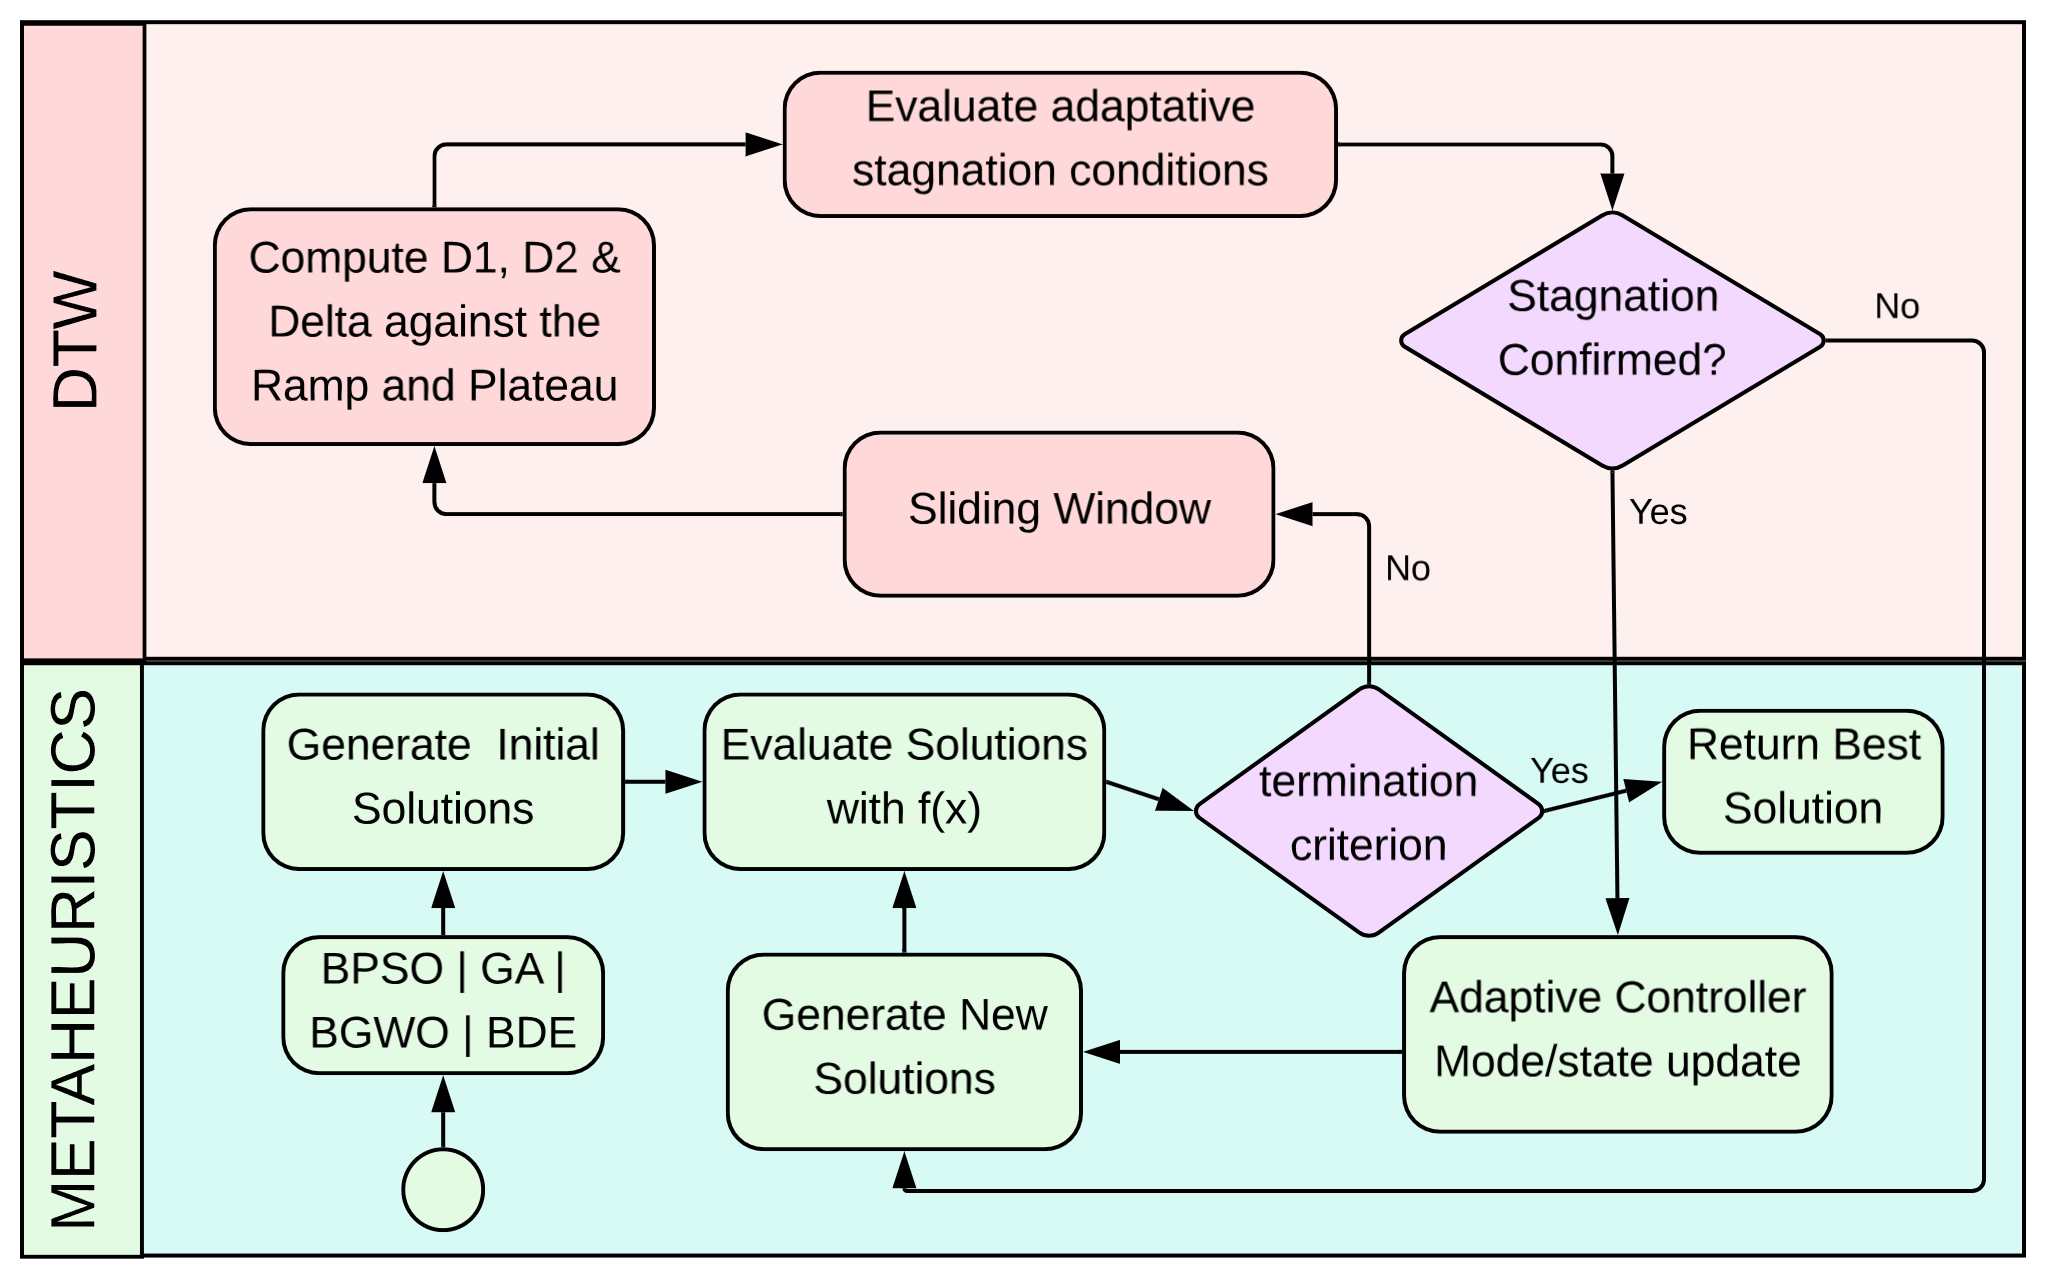
\includegraphics[width=0.88\linewidth]{architecture_diagram.png}
    \caption{Closed-loop architecture of the proposed trajectory-driven adaptive
configuration-control framework.}
    \label{fig:framework}
\end{figure}



At iteration $t$, the metaheuristic evaluates a population of candidate
solutions and records the best-so-far fitness value, denoted by $f_t^*$.
The trajectory-analysis module maintains a sliding window containing the
most recent $W$ observations of this convergence trajectory. During an
initial warm-up period, before a complete window is available, the
metaheuristic operates under its initial configuration. Once $W$
observations have been collected, the trajectory window is compared with
predefined reference patterns representing sustained progress and lack of
progress. Both adaptive strategies start in exploration. During warm-up,
the monitor supplies zero distance placeholders and marks its output as
not ready: Binary-Simple retains exploration because its plateau condition
is true, whereas Binary-Complex explicitly preserves its current state.
No DDTW comparison is made before the window is complete.
The resulting dissimilarity measures are subsequently supplied
to the adaptive controller, which determines the configuration to be used
by the metaheuristic. Specifically, the mode $s_t$ generates the fitness
observation at iteration $t$, and the controller decision computed from
that observation determines $s_{t+1}$. All switching rules below use this
observation-then-decision convention.

The architecture is deliberately modular. The trajectory-analysis module is
independent of the particular update equations of the underlying
metaheuristic, whereas the adaptive controller operates on a common
configuration interface rather than directly on algorithm-specific search
operators. Consequently, the same trajectory information can be processed
by different decision strategies and applied to different metaheuristics by
mapping the resulting control signal to their respective internal
parameters. This separation enables the trajectory-analysis mechanism,
decision logic, and underlying optimization algorithm to be studied under
a common experimental framework.


\subsection{DDTW-Based Trajectory-Pattern Analysis}
\label{sec:trajectory_analysis}

The trajectory-analysis module characterizes the recent search dynamics by
comparing the observed convergence trajectory with predefined geometric
reference patterns. Rather than representing lack of progress exclusively
through the number of consecutive iterations without improvement, the
proposed mechanism evaluates the \emph{shape} of the recent fitness
trajectory using Derivative Dynamic Time Warping (DDTW). The resulting
distances quantify whether the observed search dynamics resemble sustained
progress or a plateau and constitute the feedback information supplied to
the adaptive controller.


\subsubsection{Reference Trajectory Patterns}

Let

\begin{equation}
X_t =
\left(
f_{t-W+1}^*,
f_{t-W+2}^*,
\dots,
f_t^*
\right)
\label{eq:trajectory_window}
\end{equation}

denote the sliding window containing the $W$ most recent best-so-far fitness
values. Two synthetic reference patterns are constructed to represent
contrasting search behaviors.

The first pattern, denoted by $R_t$, represents sustained progress through
a linear trajectory with reference slope $s_{\min}>0$:

\begin{equation}
r_i =
f_{t-W+1}^*
+
s_{\min}(i-1),
\qquad i=1,\ldots,W.
\label{eq:ramp_pattern}
\end{equation}

The second pattern, denoted by $C_t$, represents the absence of progress
through a constant trajectory:

\begin{equation}
c_i =
f_{t-W+1}^*,
\qquad i=1,\ldots,W.
\label{eq:constant_pattern}
\end{equation}

Thus, $R_t$ provides a reference for sustained improvement, whereas $C_t$
represents a fully stagnant trajectory. Since the comparison is performed
on derivative representations through DDTW, the analysis emphasizes the
local evolution of the trajectory rather than its absolute fitness level.

These patterns are operational endpoints for low and sustained progress,
not a complete model of the population dynamics of all four algorithms.
The fixed slope $s_{\min}=2.0$ represents two objective-function units per
iteration. It is not estimated from the current window or fitted separately
for each algorithm or instance. Choosing the same reference makes the
comparison procedure common across algorithms, but does not establish that
this numerical slope is optimal or scale-invariant. Additive fitness shifts
are removed by first differences; multiplicative fitness rescaling is not.
The percentiles adapt to each run's distance history, so absolute distances
should not be compared directly across different objective scales. The OAT
study in Section~\ref{subsec:oat_sensitivity} does not vary this slope.


\subsubsection{Trajectory Dissimilarity Measures}

The dissimilarity between the observed trajectory and each reference pattern
is quantified using DDTW with a Sakoe--Chiba constraint of half-width
$w_{\mathrm{SC}}$:

\begin{equation}
D_R(t)
=
\operatorname{DDTW}(X_t,R_t),
\qquad
D_C(t)
=
\operatorname{DDTW}(X_t,C_t).
\label{eq:ddtw_distances}
\end{equation}

A relative trajectory indicator is additionally defined as

\begin{equation}
\Delta_t = D_R(t)-D_C(t).
\label{eq:trajectory_delta}
\end{equation}

Here, $D_R(t)$ measures the dissimilarity between the recent trajectory and
the sustained-progress reference, whereas $D_C(t)$ measures its
dissimilarity from the constant reference. Consequently, $\Delta_t$
provides a relative comparison between both patterns: negative values
indicate that the observed trajectory is closer to the progress reference,
whereas positive values indicate greater similarity to the plateau
reference.

For the constant reference, the first-difference sequence is identically
zero. Every admissible DTW path visits each observed derivative at least
once, and the diagonal path attains the sum of their absolute values.
Consequently, for the nondecreasing best-so-far window used here,
\begin{equation}
D_C(t)=\sum_{i=2}^{W}|x_i-x_{i-1}|=x_W-x_1.
\label{eq:plateau_score_identity}
\end{equation}
This identity holds for any band admitting the diagonal. Binary-Simple's
plateau score therefore measures cumulative progress within the window;
it does not uniquely distinguish detailed trajectory shapes with the same
endpoint gain. Binary-Complex additionally uses the ramp comparison and
temporal conditions. This distinction limits the interpretation of the
plateau score and explains why changing the band alone cannot change it.


\subsubsection{History-Based Adaptive Thresholds}

Because the magnitude and distribution of the trajectory distances may vary
during the optimization process, the decision thresholds are not defined as
fixed absolute values. Instead, they are dynamically estimated from the
historical distributions of the trajectory metrics.

Let $\mathcal{H}_{R}^{(t)}$, $\mathcal{H}_{C}^{(t)}$, and
$\mathcal{H}_{\Delta}^{(t)}$ denote the accumulated histories of $D_R$,
$D_C$, and $\Delta$ available at iteration $t$, respectively. The adaptive
thresholds are defined as

\begin{equation}
\theta_C(t)
=
\mathcal{P}_{p_{\mathrm{low}}}
\left(\mathcal{H}_{C}^{(t)}\right),
\label{eq:threshold_c}
\end{equation}

\begin{equation}
\theta_R(t)
=
\mathcal{P}_{p_{\mathrm{high}}}
\left(\mathcal{H}_{R}^{(t)}\right),
\label{eq:threshold_r}
\end{equation}

and

\begin{equation}
\theta_{\Delta}(t)
=
\mathcal{P}_{p_{\mathrm{high}}}
\left(\mathcal{H}_{\Delta}^{(t)}\right),
\label{eq:threshold_delta}
\end{equation}

where $\mathcal{P}_{p}(\cdot)$ denotes the $p$-th percentile of the
corresponding historical distribution. The lower percentile
$p_{\mathrm{low}}$ identifies unusually small distances to the plateau
reference, whereas the upper percentile $p_{\mathrm{high}}$ identifies
unusually large deviations from the sustained-progress reference or
correspondingly large values of the relative trajectory indicator.

This history-based formulation allows the decision criteria to adapt to the
distance distributions observed during each optimization run, reducing
their dependence on manually specified absolute distance thresholds after
the initial history-building phase. The current observation is appended
before computing percentiles, and all complete-window observations remain
in each history; there is no rolling truncation of these histories.
Percentiles use linear interpolation between sorted samples, as in
\texttt{numpy.percentile} with its default method. If fewer than ten
complete-window observations have been accumulated, the implementation uses
\begin{equation}
\theta_C=0.1W,\qquad\theta_R=0.5W,\qquad\theta_\Delta=0.3W.
\label{eq:initial_thresholds}
\end{equation}
Thus, with $W=200$, the first complete window is observed at iteration 200
and history-based percentiles begin at iteration 209. The same fixed
thresholds are returned as placeholders during warm-up, together with a
not-ready flag. The consecutive-no-improvement counter is zero for the
first post-iteration observation; subsequently it increments on a tie or
decrease and resets on a strict improvement. The persistence counter
increments only when all three stagnation conditions hold and otherwise
resets to zero.


\subsection{Adaptive Configuration-Control Strategies}
\label{sec:adaptation_strategies}

The trajectory information described above is translated into changes in
the search configuration through two binary adaptive control strategies.
Both strategies operate on the same trajectory information and configuration
interface but differ in the complexity of the decision mechanism used to
trigger transitions between exploration and exploitation.

For binary control, let

\begin{equation}
s_t \in \{0,1\}
\end{equation}

denote the search mode at iteration $t$, where $s_t=0$ selects the
exploitation-oriented configuration and $s_t=1$ selects the
exploration-oriented configuration. The corresponding parameter vector can
be expressed as

\begin{equation}
\boldsymbol{\theta}_t =
\begin{cases}
\boldsymbol{\theta}^{\mathrm{exploit}}, & s_t=0,\\
\boldsymbol{\theta}^{\mathrm{explore}}, & s_t=1,
\end{cases}
\label{eq:binary_config}
\end{equation}

where $\boldsymbol{\theta}^{\mathrm{exploit}}$ and
$\boldsymbol{\theta}^{\mathrm{explore}}$ denote the two predefined
algorithm-specific parameter configurations. Their numerical values for
BPSO, GA, BGWO, and BDE are reported in the Experimental Setup.


\subsubsection{Binary-Simple Strategy}

Binary-Simple constitutes the lowest-complexity trajectory-driven controller.
It uses only the distance to the plateau reference and does not require
temporal persistence of the detected condition. The decision rule is

\begin{equation}
s_{t+1} =
\begin{cases}
1, & D_C(t) \leq \theta_C(t),\\
0, & \text{otherwise}.
\end{cases}
\label{eq:binary_simple}
\end{equation}

Therefore, when the recent trajectory becomes unusually similar to the
plateau reference with respect to its historical behavior, the controller
selects the exploration-oriented configuration. Otherwise, the
exploitation-oriented configuration is used.


\subsubsection{Binary-Complex Strategy}

Binary-Complex extends the previous controller by combining multiple
trajectory and progress conditions with temporal persistence and asymmetric
switching. Three conditions are evaluated:

\begin{align}
C_{\mathrm{noimp}}(t) &:\
\ell_{\mathrm{noimp}}(t) \geq \pi_{\max},
\label{eq:cond_noimp}\\
C_{\mathrm{plateau}}(t) &:\
D_C(t) \leq \theta_C(t),
\label{eq:cond_plateau}\\
C_{\mathrm{progress}}(t) &:\
\left[D_R(t) \geq \theta_R(t)\right]
\lor
\left[\Delta_t \geq \theta_{\Delta}(t)\right].
\label{eq:cond_progress}
\end{align}

Here, $\ell_{\mathrm{noimp}}(t)$ denotes the number of consecutive iterations
without improvement in the best-so-far fitness, and $\pi_{\max}$ defines the
minimum number of such iterations required to provide explicit evidence of
lack of progress. The second condition identifies trajectories unusually
close to the plateau reference, whereas the third captures trajectories that
are unusually distant from the sustained-progress pattern, either directly
through $D_R(t)$ or relatively through $\Delta_t$.

Let

\begin{equation}
C_{\mathrm{stag}}(t)
=
C_{\mathrm{noimp}}(t)
\land
C_{\mathrm{plateau}}(t)
\land
C_{\mathrm{progress}}(t)
\label{eq:composite_stagnation}
\end{equation}

denote the composite stagnation condition. A transition from exploitation
to exploration is performed only when $C_{\mathrm{stag}}(t)$ remains
satisfied for $\tau_{\mathrm{pat}}$ consecutive iterations. In contrast, a
strict improvement in the best-so-far fitness immediately returns the
algorithm to the exploitation-oriented configuration:

\begin{equation}
s_{t+1} =
\begin{cases}
1,
&
s_t=0
\;\land\;
C_{\mathrm{stag}}(k)=1
\quad
\forall k\in
\{t-\tau_{\mathrm{pat}}+1,\ldots,t\},
\\[2mm]
0,
&
s_t=1
\;\land\;
f_t^*>f_{t-1}^*,
\\[2mm]
s_t,
&
\text{otherwise}.
\end{cases}
\label{eq:binary_complex}
\end{equation}

This asymmetric hysteresis requires sustained evidence of stagnation before
activating exploration, thereby reducing sensitivity to transient trajectory
fluctuations. Conversely, once the exploratory configuration produces a
strict improvement in the best-so-far solution, the controller immediately
returns to exploitation for the next iteration so that the newly
discovered region can be intensified. These transitions are enabled only
after the monitor becomes ready; during warm-up Binary-Complex retains
the initial exploration mode. The persistence counter is updated by the
monitor on every ready observation, independently of the controller mode.



%%%%%%%%%%%%%%%%%%%%%%%%%%%%%%%%%%%%%%%%%%
\section{Experimental Setup}
\label{sec:experimental_setup}

\subsection{Environment}
\label{sec:computational_environment}

The computational experiments were conducted within a Python 3.11 (Python Software Foundation, Wilmington, DE, USA) execution environment, leveraging the high-throughput capabilities of the Océano High-Performance Computing (HPC) Cluster at the \textit{Pontificia Universidad Católica de Valparaíso (PUCV)}. Workloads were orchestrated via the Slurm Workload Manager across high-density Dell PowerEdge R640 compute nodes (equipped with dual Intel\textregistered\ Xeon\textregistered\ Scalable processors and ECC DDR4 RAM). Vectorized routines were accelerated using NumPy, and preliminary script prototyping was carried out on a dedicated multi-core workstation.

\subsection{Benchmark Instances and Metaheuristic Configurations}
\label{sec:instances}

The proposed framework is evaluated using benchmark instances from the
Chu--Beasley Multidimensional Knapsack Problem (MKP) test suite
\cite{chu1998genetic}, available through the OR-Library. Nine benchmark
groups are considered, corresponding to the combinations of three numbers
of constraints ($m\in\{5,10,30\}$) and three problem dimensions
($n\in\{100,250,500\}$). Three instances are selected from each group
using the fixed, zero-based indices $0$, $15$, and $29$, yielding 27
evaluation instances. Index $0$ retains the original benchmark cases for
backward comparison; the two additional indices extend coverage within
each group. This deterministic selection is not a random or exhaustive
sample of the 30 instances available in each group.
Throughout the results, \texttt{mknapcb}$g$[$i$] denotes index $i$ from
benchmark group $g$. Table~\ref{tab:instances} summarizes the dimensions
and the known optimal objective values for all selected cases.

\begin{table}[htbp]
\centering
\small
\caption{The nine MKP benchmark groups and the three selected instances per
group (zero-based indices $0$, $15$, and $29$): 27 instances in total.}
\label{tab:instances}
\begin{tabular}{@{}lccrrr@{}}
\toprule
\textbf{Group} & \textbf{$m$} & \textbf{$n$} &
\textbf{$f^*$ (idx 0)} & \textbf{$f^*$ (idx 15)} & \textbf{$f^*$ (idx 29)} \\
\midrule
mknapcb1 & 5 & 100 & 24\,381 & 42\,927 & 59\,965 \\
mknapcb2 & 5 & 250 & 59\,312 & 110\,256 & 154\,662 \\
mknapcb3 & 5 & 500 & 120\,130 & 220\,514 & 299\,904 \\
mknapcb4 & 10 & 100 & 23\,064 & 42\,995 & 60\,633 \\
mknapcb5 & 10 & 250 & 59\,187 & 110\,841 & 149\,704 \\
mknapcb6 & 10 & 500 & 117\,726 & 215\,013 & 307\,014 \\
mknapcb7 & 30 & 100 & 21\,946 & 41\,058 & 60\,603 \\
mknapcb8 & 30 & 250 & 56\,693 & 107\,246 & 149\,572 \\
mknapcb9 & 30 & 500 & 115\,868 & 215\,762 & 300\,460 \\
\bottomrule
\end{tabular}
\end{table}

Candidate solutions that violate one or more resource constraints are
restored to feasibility using a greedy repair procedure. Infeasible
solutions are first repaired by iteratively removing low-density items until
all constraints are satisfied. A subsequent insertion phase considers
high-density items and adds them whenever their inclusion preserves
feasibility. The same repair procedure is applied to all metaheuristics and
adaptive variants to avoid introducing algorithm-dependent differences in
constraint handling.


\subsubsection{Metaheuristic Configurations}
\label{sec:mh_config}

All four metaheuristics use a population size of $N=20$ and a computational
budget of $T=2000$ iterations. Each experimental condition is evaluated over
$R=31$ independent runs. These settings are kept fixed across algorithms,
instances, and control strategies.

Four experimental variants are considered for each metaheuristic:
Vanilla-Exploitation, Vanilla-Exploration, Binary-Simple, and Binary-Complex.
The two Vanilla variants maintain a fixed exploitation- or
exploration-oriented parameter configuration throughout the entire run,
whereas Binary-Simple and Binary-Complex dynamically switch between the same
two configurations according to the trajectory-driven control mechanisms
described in Section~\ref{sec:adaptation_strategies}. For BPSO, BGWO, and
BDE, continuous internal quantities are mapped to binary decisions using a
sigmoid transfer function. Table~\ref{tab:mh_params} reports the parameter
values defining the two configurations for each metaheuristic.

\begin{table}[htbp]
\centering
\caption{Exploration- and exploitation-oriented parameter configurations
used for each metaheuristic.}
\label{tab:mh_params}
\begin{tabular}{@{}l l l l@{}}
\toprule
\textbf{MH} &
\textbf{Parameter} &
\textbf{Exploitation} &
\textbf{Exploration} \\
\midrule

\multirow{3}{*}{BPSO}
  & $w$   & 0.729   & 0.9 \\
  & $c_1$ & 1.49445 & 2.5 \\
  & $c_2$ & 1.49445 & 0.5 \\

\midrule

\multirow{2}{*}{GA}
  & $p_c$ & 0.9  & 0.6 \\
  & $p_m$ & 0.01 & 0.15 \\

\midrule

BGWO
  & $a$ & 0.5 & 2.0 \\

\midrule

\multirow{2}{*}{BDE}
  & $F$  & 0.5 & 0.9 \\
  & $CR$ & 0.9 & 0.3 \\

\bottomrule
\end{tabular}
\end{table}

The parameter configurations were defined using established parameter
settings and search-behavior principles reported for the corresponding
metaheuristics \cite{clerc2002particle,goldberg1989genetic,
mirjalili2014grey,storn1997differential}. The exploitation-oriented profiles
favor stronger convergence toward promising regions, whereas the
exploration-oriented profiles modify the corresponding parameters to promote
greater diversification. Specifically, the BPSO exploration profile increases
the inertia and cognitive contribution while reducing the social component;
the GA profile increases the mutation probability while reducing the
crossover probability; the BGWO profile uses a larger value of the
exploration-related coefficient $a$; and the BDE profile increases the
differential scaling factor while reducing the crossover rate. These
configurations are kept unchanged across all benchmark instances. The
cited studies motivate the parameter roles and the direction of these
changes; they do not certify the numerical profiles as optimal for MKP.
In the evaluated implementation, these profiles are fixed constants rather
than outputs of a per-instance fitting procedure. No systematic search over
profile values or separate training/validation phase is reported here.
Accordingly, the experiment evaluates switching between two prescribed
profiles, not the optimality of their selection.


\subsection{DDTW Trajectory-Analysis and Controller Parameters}
\label{sec:dtw_config}

The DDTW-based trajectory-analysis module and both adaptive controllers use
a common parameterization throughout the complete experimental evaluation.
No instance- or metaheuristic-specific adjustment of these parameters is
performed. Table~\ref{tab:dtw_params} summarizes the corresponding values.

\begin{table}[htbp]
\centering
\caption{Parameters of the DDTW-based trajectory-analysis module and adaptive
controllers.}
\label{tab:dtw_params}
\begin{tabular}{@{}l c l@{}}
\toprule
\textbf{Parameter} & \textbf{Value} & \textbf{Description} \\
\midrule
$W$                  & 200 & Sliding-window length \\
$w_{\mathrm{SC}}$    & 2   & Sakoe--Chiba band half-width \\
$s_{\min}$           & 2.0 & Reference slope for sustained progress \\
$p_{\mathrm{low}}$   & 40  & Percentile defining $\theta_C$ \\
$p_{\mathrm{high}}$  & 60  & Percentile defining $\theta_R$ and $\theta_\Delta$ \\
$\pi_{\max}$         & 5   & Minimum consecutive iterations without improvement \\
$\tau_{\mathrm{pat}}$ & 3  & Persistence required for stagnation confirmation \\
\bottomrule
\end{tabular}
\end{table}

The percentile values $p_{\mathrm{low}}=40$ and
$p_{\mathrm{high}}=60$ are used to dynamically derive the trajectory
thresholds from the historical distributions accumulated during each run.
Binary-Simple uses only the plateau-distance condition
$D_C(t)\leq\theta_C(t)$, whereas Binary-Complex combines the three conditions
defined in Section~\ref{sec:adaptation_strategies} together with the
no-improvement threshold $\pi_{\max}$ and persistence parameter
$\tau_{\mathrm{pat}}$.

The same values of $W$, $w_{\mathrm{SC}}$, $s_{\min}$,
$p_{\mathrm{low}}$, and $p_{\mathrm{high}}$ are used by both adaptive
strategies. Consequently, differences between Binary-Simple and
Binary-Complex arise from their decision logic rather than from different
parameterizations of the underlying trajectory-analysis module.


\subsection{Experimental Protocol}
\label{sec:protocol}

Each experimental run corresponds to the application of one metaheuristic under one configuration-control strategy to a given MKP instance. The same
population size, iteration budget, repair mechanism, and trajectory-analysis
parameters are maintained across the corresponding experimental conditions.
The expanded campaign contains $27\times4\times4=432$ experimental
conditions and $432\times31=13\,392$ runs, with 31 independent replicates
per condition. All 432 serialized
fitness arrays contain 31 finite values; the solution-quality tables were
checked against these arrays before incorporating the expanded results.
This campaign is separate from the one-factor-at-a-time sensitivity
experiment in Section~\ref{subsec:oat_sensitivity}.
Algorithm~\ref{alg:run} summarizes the procedure for a single independent
run.
\begin{algorithm}[p]
\caption{Single run with explicit configuration-switching rules.}
\label{alg:run}
\footnotesize
\begin{algorithmic}[1]
\Require Instance $\mathcal I$, algorithm $\mathcal A$, strategy $\mathcal C$,
profiles $\Pi_0,\Pi_1$, seed $q$, population $N$, budget $T$, monitor settings
\Ensure Best solution and in-memory fitness, diagnostic, and applied-mode histories
\State Initialize \texttt{numpy.random.default\_rng} with seed $q$
\State Generate, repair, and evaluate the initial population of size $N$
\State Initialize the incumbent $x^*$ and empty post-iteration histories
\State Initialize monitor history, no-improvement count $\ell=0$, persistence $g=0$
\State Set $s_1=0$ for Vanilla-Exploitation; otherwise set $s_1=1$
\State Apply profile $\Pi_{s_1}$ after population initialization
\For{$t=1,\ldots,T$}
  \State Generate, repair, and evaluate candidates using profile $\Pi_{s_t}$
  \State Update $x^*$ and obtain best-so-far fitness $f_t^*$
  \State Record $f_t^*$ and the mode $s_t$ actually used in this iteration
  \State Set $s_{t+1}\gets s_t$
  \If{$\mathcal C$ is adaptive}
    \State Obtain monitor output $\mathbf z_t$ using Algorithm~\ref{alg:monitor}
    \If{$\mathcal C$ is Binary-Simple}
      \State $s_{t+1}\gets\mathbb{1}[D_C(t)\leq\theta_C(t)]$
      \Comment{Includes warm-up placeholders}
    \ElsIf{the monitor is ready}
      \If{$s_t=0$ and $g\geq\tau_{\mathrm{pat}}$}
        \State $s_{t+1}\gets1$
      \ElsIf{$s_t=1$ and $\ell=0$}
        \State $s_{t+1}\gets0$
      \EndIf
    \EndIf
    \State Apply profile $\Pi_{s_{t+1}}$ for the next iteration
    \State Record diagnostics and count a transition only if $s_t=0$, $s_{t+1}=1$
  \EndIf
\EndFor
\State \Return $x^*$, final fitness, and the three in-memory histories
\end{algorithmic}
\end{algorithm}

\begin{algorithm}[p]
\caption{Monitor update: derivatives, thresholds, and temporal confirmation.}
\label{alg:monitor}
\footnotesize
\begin{algorithmic}[1]
\Require Current observation $f_t^*$, history, $W,w_{\mathrm{SC}},s_{\min}$,
percentiles $p_{\mathrm{low}},p_{\mathrm{high}}$, $\pi_{\max},\tau_{\mathrm{pat}}$
\Ensure Ready flag, $D_R,D_C,\Delta$, thresholds, $\ell$, $g$, and fire flag
\If{the history is nonempty and $f_t^*$ is not greater than its last value}
  \State Increment $\ell$ and clamp $f_t^*$ to the last best-so-far value
\Else
  \State $\ell\gets0$
\EndIf
\State Append $f_t^*$ to the post-iteration best-so-far history
\If{fewer than $W$ observations are available}
  \State Return not-ready, zero distances and $\Delta$, thresholds
  $(0.1W,0.5W,0.3W)$, $\ell$, $g=0$, fire=false
\EndIf
\State Extract the most recent $W$ observations as $X_t$
\State Construct $R_t,C_t$ using Equations~\ref{eq:ramp_pattern}--\ref{eq:constant_pattern}
\State First-difference $X_t,R_t,C_t$ using Equation~\ref{eq:first_difference}
\For{each reference derivative $B'\in\{R'_t,C'_t\}$}
  \State Initialize $D[0{:}W,0{:}W]\gets\infty$ and $D[0,0]\gets0$
  \For{$i=1,\ldots,W$}
    \For{$j=\max(1,i-w_{\mathrm{SC}}),\ldots,\min(W,i+w_{\mathrm{SC}})$}
      \State $D[i,j]\gets|x'_i-b'_j|+\min\{D[i-1,j],D[i,j-1],D[i-1,j-1]\}$
    \EndFor
  \EndFor
  \State Store $D[W,W]$ as the corresponding distance $D_R$ or $D_C$
\EndFor
\State $\Delta\gets D_R-D_C$
\State Append these values to their respective complete-window histories
\If{at least ten complete-window observations are available}
  \State Compute thresholds from Equations~\ref{eq:threshold_c}--\ref{eq:threshold_delta}
  \Comment{Include current sample; linear percentiles}
\Else
  \State Set thresholds to $(0.1W,0.5W,0.3W)$
\EndIf
\State $C\gets[\ell\geq\pi_{\max}]\land[D_C\leq\theta_C]$
\State $C\gets C\land([D_R\geq\theta_R]\lor[\Delta\geq\theta_\Delta])$
\If{$C$ is true}
  \State $g\gets g+1$
\Else
  \State $g\gets0$
\EndIf
\State Return ready, distances, thresholds, $\ell,g$, and fire=$[g\geq\tau_{\mathrm{pat}}]$
\end{algorithmic}
\end{algorithm}

\subsection{Implementation and Reproduction Details}
\label{subsec:reproduction}

Algorithms~\ref{alg:run} and~\ref{alg:monitor} expose the decision sequence;
Appendix~\ref{sec:appendix_reproduction} gives executable reproduction
commands and the output structure. A public, permanently archived release
of the complete code and data is not identified in this manuscript.

For each condition, the HPC runner assigns seed $q=e+1$ to zero-based run
index $e=0,\ldots,30$. The same seed list $1,\ldots,31$ is used across the
four strategies and four algorithms, with a fresh NumPy generator for each
run. Results are sorted by run index before serialization, not by worker
completion time. This defines the pairing used in local comparisons;
different algorithms may consume different random draws even at the same
seed. The explicit instance indices $0,15,29$ are independent of this
run-seed convention and are not randomly sampled in the reported campaign.

The runner creates full fitness, monitor, and applied-mode histories in
memory. However, the saved campaign JSON files contain only final fitness,
runtime, transition counts, gains, summary statistics, and configuration
metadata. They do not retain the full per-iteration histories, explicit
seed arrays, or a source commit hash. Consequently, aggregate tables can
be regenerated from these files, whereas synchronized controller traces
require rerunning the experiment and saving the in-memory histories.
Exact runtime reproduction additionally depends on hardware, process
allocation, and the software environment; an iteration budget is not a
hardware-independent wall-clock budget.

\section{Results}
\label{sec:results}

This section presents the experimental results obtained for the four
metaheuristics (BPSO, GA, BGWO, and BDE) across the 27 MKP benchmark
instances (three selected indices per group). The analysis considers three complementary aspects: solution
quality, statistical evidence, and computational overhead. In addition,
the switching behavior of the adaptive controllers is examined to provide
insight into how the trajectory-driven mechanisms operate during the search.
Each experimental condition comprises $R=31$ independent runs.


   The MFSS results cannot be interpreted as a direct performance comparison with the methods evaluated in this study. The
 MFSS experiments used ten independent runs and a time-based budget, whereas our experiments use 31 runs and a budget of 2,000
 iterations. In addition, the ID~0 objective or best-known values reported for four overlapping benchmark groups differ from
 the values listed in Table~\ref{tab:instances}. Therefore, instance-level equivalence has not been established for those
 groups, and no statistical or superiority claim is made from the published MFSS values.
% ============================================================
\subsection{Solution Quality}
\label{subsec:solution_quality}

Optimization performance is first assessed using the final best-so-far
objective values obtained over the independent runs. For each experimental
condition, the best fitness value ($f_{\mathrm{best}}$), mean final fitness
($\bar{f}$), standard deviation ($\sigma$), and relative optimality gap are
reported. Since the global optimum $f^*$ is known for all benchmark
instances, the mean relative optimality gap is computed as

\begin{equation}
    \text{Gap}(\%) =
    \left(
    \frac{f^*-\bar{f}}{f^*}
    \right)\times100.
    \label{eq:gap_results}
\end{equation}

Lower Gap values therefore indicate better average solution quality, with
$\text{Gap}=0$ corresponding to the known optimum.

To preserve direct comparison with the original nine-case evaluation,
Tables~\ref{tab:calidad_mknapcb1_0}, \ref{tab:calidad_mknapcb5_0}, and
\ref{tab:calidad_mknapcb9_0} retain three representative index-$0$ cases:
\texttt{mknapcb1[0]} ($n=100$, $m=5$),
\texttt{mknapcb5[0]} ($n=250$, $m=10$), and
\texttt{mknapcb9[0]} ($n=500$, $m=30$).
Table~\ref{tab:gap_all_instances} summarizes the enlarged 27-instance
evaluation. Complete per-instance solution-quality results for the
remaining 24 cases are provided in Appendix~\ref{sec:appendix_tables}.

% --- Representative Instance 1 ---
% --- Solution Quality: mknapcb1 (Instance 0) ---
\begin{table}[htbp]
  \centering
  \small
  \caption{Solution quality on \textbf{mknapcb1} (inst. 0, $n=100$, $m=5$, $f^*=24\,381$).}
  \label{tab:calidad_mknapcb1_0}
  \begin{tabular}{lrrrr}
    \toprule
    \textbf{MH -- Variant} &
    \textbf{Best Fitness} &
    \textbf{Average} &
    \textbf{Std.} &
    \textbf{Gap (\%)} \\
    \midrule
    BPSO -- Vanilla Exploitation & \textbf{24381} &         24256.58 &  46.29 &         0.51 \\
    BPSO -- Vanilla Exploration  & \textbf{24381} & \textbf{24343.65} &  26.75 & \textbf{0.15} \\
    BPSO -- Binary-Simple        & \textbf{24381} &         24329.74 &  32.18 &         0.21 \\
    BPSO -- Binary-Complex       & \textbf{24381} &         24330.87 &  32.34 &         0.21 \\
    \midrule
    GA -- Vanilla Exploitation   &          24373 &         24283.26 &  55.41 &         0.40 \\
    GA -- Vanilla Exploration    & \textbf{24381} &         24309.35 &  31.09 &         0.29 \\
    GA -- Binary-Simple          &          24373 &         24307.23 &  36.21 &         0.30 \\
    GA -- Binary-Complex         & \textbf{24381} & \textbf{24316.90} &  38.86 & \textbf{0.26} \\
    \midrule
    BGWO -- Vanilla Exploitation &          24259 & \textbf{24197.77} &  33.65 & \textbf{0.75} \\
    BGWO -- Vanilla Exploration  & \textbf{24327} &         24190.19 &  38.87 &         0.78 \\
    BGWO -- Binary-Simple        & \textbf{24327} &         24181.58 &  52.96 &         0.82 \\
    BGWO -- Binary-Complex       & \textbf{24327} &         24191.71 &  36.68 &         0.78 \\
    \midrule
    BDE -- Vanilla Exploitation  &          24330 &         24234.52 &  79.08 &         0.60 \\
    BDE -- Vanilla Exploration   & \textbf{24381} & \textbf{24322.32} &  30.15 & \textbf{0.24} \\
    BDE -- Binary-Simple         & \textbf{24381} &         24306.39 &  41.38 &         0.31 \\
    BDE -- Binary-Complex        &          24337 &         24288.06 &  27.59 &         0.38 \\
    \bottomrule
  \end{tabular}
\end{table}

% --- Representative Instance 5 ---
% --- Solution Quality: mknapcb5 (Instance 0) ---
\begin{table}[htbp]
  \centering
  \small
  \caption{Solution quality on \textbf{mknapcb5} (inst. 0, $n=250$, $m=10$, $f^*=59\,187$).}
  \label{tab:calidad_mknapcb5_0}
  \begin{tabular}{lrrrr}
    \toprule
    \textbf{MH -- Variant} &
    \textbf{Best Fitness} &
    \textbf{Average} &
    \textbf{Std.} &
    \textbf{Gap (\%)} \\
    \midrule
    BPSO -- Vanilla Exploitation &          58285 &         57676.74 & 207.82 &         2.55 \\
    BPSO -- Vanilla Exploration  & \textbf{58564} & \textbf{58288.10} & 109.54 & \textbf{1.52} \\
    BPSO -- Binary-Simple        &          58527 &         58224.81 & 148.57 &         1.63 \\
    BPSO -- Binary-Complex       &          58439 &         58186.45 & 123.58 &         1.69 \\
    \midrule
    GA -- Vanilla Exploitation   & \textbf{59094} & \textbf{58830.06} & 130.21 & \textbf{0.60} \\
    GA -- Vanilla Exploration    &          58573 &         58206.61 & 144.26 &         1.66 \\
    GA -- Binary-Simple          &          58966 &         58617.29 & 193.96 &         0.96 \\
    GA -- Binary-Complex         &          58947 &         58690.10 & 152.55 &         0.84 \\
    \midrule
    BGWO -- Vanilla Exploitation & \textbf{58148} & \textbf{57569.81} & 187.46 & \textbf{2.73} \\
    BGWO -- Vanilla Exploration  &          57747 &         57468.90 & 128.10 &         2.90 \\
    BGWO -- Binary-Simple        &          58058 &         57532.39 & 183.26 &         2.80 \\
    BGWO -- Binary-Complex       &          57747 &         57464.65 & 147.07 &         2.91 \\
    \midrule
    BDE -- Vanilla Exploitation  &          58807 &         58394.58 & 193.71 &         1.34 \\
    BDE -- Vanilla Exploration   &          58938 &         58628.68 & 139.05 &         0.94 \\
    BDE -- Binary-Simple         & \textbf{58971} &         58671.94 & 156.25 &         0.87 \\
    BDE -- Binary-Complex        &          58961 & \textbf{58747.71} & 111.18 & \textbf{0.74} \\
    \bottomrule
  \end{tabular}
\end{table}

% --- Representative Instance 9 ---
% --- Solution Quality: mknapcb9 (Instance 0) ---
\begin{table}[htbp]
  \centering
  \small
  \caption{Solution quality on \textbf{mknapcb9} (inst. 0, $n=500$, $m=30$, $f^*=115\,868$).}
  \label{tab:calidad_mknapcb9_0}
  \begin{tabular}{lrrrr}
    \toprule
    \textbf{MH -- Variant} &
    \textbf{Best Fitness} &
    \textbf{Average} &
    \textbf{Std.} &
    \textbf{Gap (\%)} \\
    \midrule
    BPSO -- Vanilla Exploitation &         111723 &        111259.61 & 268.02 &         3.98 \\
    BPSO -- Vanilla Exploration  & \textbf{112766} & \textbf{112194.90} & 248.78 & \textbf{3.17} \\
    BPSO -- Binary-Simple        &         112527 &        112177.81 & 230.27 &         3.18 \\
    BPSO -- Binary-Complex       &         112752 &        112155.48 & 284.79 &         3.20 \\
    \midrule
    GA -- Vanilla Exploitation   & \textbf{115205} & \textbf{114841.97} & 207.64 & \textbf{0.89} \\
    GA -- Vanilla Exploration    &         112886 &        112113.00 & 327.65 &         3.24 \\
    GA -- Binary-Simple          &         114665 &        113450.29 & 579.15 &         2.09 \\
    GA -- Binary-Complex         &         114647 &        114272.58 & 244.37 &         1.38 \\
    \midrule
    BGWO -- Vanilla Exploitation &         111836 &        111465.45 & 183.47 &         3.80 \\
    BGWO -- Vanilla Exploration  &         111784 &        111389.61 & 166.71 &         3.87 \\
    BGWO -- Binary-Simple        & \textbf{111960} & \textbf{111484.71} & 210.11 & \textbf{3.78} \\
    BGWO -- Binary-Complex       &         111803 &        111412.16 & 209.34 &         3.85 \\
    \midrule
    BDE -- Vanilla Exploitation  &         113731 &        112748.32 & 449.92 &         2.69 \\
    BDE -- Vanilla Exploration   &         113456 &        112854.19 & 298.97 &         2.60 \\
    BDE -- Binary-Simple         & \textbf{114342} &        113489.10 & 381.88 &         2.05 \\
    BDE -- Binary-Complex        &         114152 & \textbf{113496.81} & 334.71 & \textbf{2.05} \\
    \bottomrule
  \end{tabular}
\end{table}


\begin{table}[htbp]
  \centering
  \small
  \caption{Mean relative optimality gap (\%) across all 27 instances,
  with each instance weighted equally. These are descriptive averages of
  per-instance mean gaps, not gaps calculated from pooled raw fitness.
  Bold indicates the lowest average gap within each metaheuristic.}
  \label{tab:gap_all_instances}
  \begin{tabular}{lrrrr}
    \toprule
    Algorithm & V-Exploit & V-Explore & Bin-Simple & Bin-Complex \\
    \midrule
    BPSO & 2.44 & \textbf{1.64} & 1.73 & 1.72 \\
    GA & \textbf{0.41} & 1.75 & 0.86 & 0.52 \\
    BGWO & \textbf{2.73} & 2.79 & 2.77 & 2.77 \\
    BDE & 1.51 & 0.94 & \textbf{0.75} & 0.77 \\
    \bottomrule
  \end{tabular}
\end{table}

The extended sample retains the algorithm-dependent pattern, but does not
support uniform dominance by the more complex controller. Across all 27
instances, BDE's mean gap is $0.77\%$ with Binary-Complex, compared with
$1.51\%$ for Vanilla-Exploitation and $0.94\%$ for Vanilla-Exploration;
Binary-Simple has a slightly lower descriptive average ($0.75\%$).
For GA, Binary-Complex ($0.52\%$) improves on Binary-Simple ($0.86\%$)
and Vanilla-Exploration ($1.75\%$), while Vanilla-Exploitation remains
stronger on average ($0.41\%$). For BPSO, Vanilla-Exploration has the
lowest average gap ($1.64\%$), versus $1.72\%$ for Binary-Complex.
BGWO's average gaps are close across strategies ($2.73\%$--$2.79\%$).
These summaries include the new indices $15$ and $29$ and complement,
rather than replace, the individual-case results.

The index-$0$ results reveal that the relative performance of the four variants depends
on both the underlying metaheuristic and the benchmark instance. Consequently,
no single fixed configuration consistently dominates across all experimental
conditions.

For BPSO, the exploration-oriented configuration generally provides stronger
performance than the fixed exploitation profile as problem size increases.
On \texttt{mknapcb5[0]}, Vanilla-Exploration achieves a mean gap of $1.52\%$,
compared with $2.55\%$ for Vanilla-Exploitation, while Binary-Simple and
Binary-Complex remain close to the exploration-oriented baseline, with gaps
of $1.63\%$ and $1.69\%$, respectively. A similar pattern is observed on
\texttt{mknapcb9[0]}, where Vanilla-Exploration, Binary-Simple, and
Binary-Complex obtain gaps of $3.17\%$, $3.18\%$, and $3.20\%$,
respectively, compared with $3.98\%$ for Vanilla-Exploitation. Thus, the
adaptive variants avoid the comparatively weaker behavior of the fixed
exploitation profile on these larger BPSO instances while remaining
competitive with the stronger fixed configuration.

GA exhibits a different pattern. Vanilla-Exploitation performs particularly
well on the larger representative instances, achieving gaps of $0.60\%$ on
\texttt{mknapcb5[0]} and $0.89\%$ on \texttt{mknapcb9[0]}. Binary-Complex obtains
the strongest performance among the remaining variants on both instances,
with gaps of $0.84\%$ and $1.38\%$, respectively, but does not surpass the
favorable fixed exploitation configuration. At the same time, Binary-Complex
substantially improves upon Vanilla-Exploration on \texttt{mknapcb9[0]},
reducing the mean gap from $3.24\%$ to $1.38\%$. These results illustrate
that the effectiveness of adaptive control depends on the behavior of the
underlying metaheuristic and that a favorable fixed configuration can remain
difficult to outperform in specific conditions.

For BGWO, differences among the four variants are comparatively small.
On \texttt{mknapcb5[0]}, mean gaps range from $2.73\%$ to $2.91\%$, whereas
on \texttt{mknapcb9[0]} they range from $3.78\%$ to $3.87\%$. Binary-Simple
achieves the lowest mean gap on \texttt{mknapcb9[0]}, while
Vanilla-Exploitation performs best on \texttt{mknapcb5[0]}. The comparatively
narrow performance range suggests that configuration changes have a more
limited effect on BGWO under the evaluated conditions.

The clearest benefits of trajectory-driven adaptation among the
representative instances are observed for BDE. On \texttt{mknapcb5[0]},
Binary-Complex achieves the lowest mean gap ($0.74\%$), improving upon
Vanilla-Exploitation ($1.34\%$), Vanilla-Exploration ($0.94\%$), and
Binary-Simple ($0.87\%$). On \texttt{mknapcb9[0]}, both adaptive strategies
achieve a gap of approximately $2.05\%$, compared with $2.69\%$ and
$2.60\%$ for Vanilla-Exploitation and Vanilla-Exploration, respectively.
This behavior indicates that BDE benefits particularly from dynamically
alternating between the two predefined configurations under the proposed
trajectory-driven control mechanism.

Overall, the descriptive results support two main observations. First, the
preferred fixed configuration varies across metaheuristics and benchmark
conditions, reinforcing the motivation for online configuration control
rather than reliance on a single predefined search profile. Second, the
trajectory-driven variants remain competitive across the evaluated
conditions and provide clear improvements in several cases, particularly
for BDE and for GA when compared with its exploration-oriented baseline.
The following statistical analysis examines whether these observed
differences are supported by inferential evidence.

In the published MKP evaluation, the LBLP strategy reached 20 of 30 known
optima, while QPSO was reported to attain 21 of 30 best-known values
\cite{vega2024lblp}. In our study,
Binary-Complex achieved a mean gap of $0.74\%$ for BDE on
\texttt{mknapcb5[0]}, compared with $0.94\%$ for the best fixed profile; on
\texttt{mknapcb9[0]}, the corresponding gaps were $2.05\%$ and $2.60\%$.
These outcomes provide context only: the benchmark cases, algorithms,
reported metrics, and evaluation budgets differ, so they do not establish
which method performs better.

To illustrate search-trajectory progression for the two binary variants,
Figures~\ref{fig:convergence_mknapcb1_binary_simple} and
\ref{fig:convergence_mknapcb1_binary_complex} show the three
\texttt{mknapcb1} instances, with indices $0$, $15$, and $29$ from top to
bottom. For each plotted variant, metaheuristic, and instance, the curve is
the run with the best final fitness among that condition's 31 independent
runs. These selected runs illustrate trajectories only: they are neither
means nor typical behavior and provide no evidence of causal effects or
method superiority; statistical conclusions continue to rely on all 31
runs per condition. Corresponding selected-run plots for \texttt{mknapcb5}
and \texttt{mknapcb9} are provided in Appendix~\ref{subsec:appendix_convergence_trajectories}.

For conciseness and readability, convergence illustrations are limited
to three benchmark groups (\texttt{mknapcb1}, \texttt{mknapcb5}, and
\texttt{mknapcb9}), with three instances per group. Displaying trajectories
for every experimental condition would substantially expand the manuscript
and supplementary material. This restriction concerns only the graphical
illustrations; the tabulated descriptive and statistical analyses cover
all 27 evaluated instances. Additional convergence plots can be prepared
upon request.

   \begin{figure}[htbp]
     \centering
     \includegraphics[width=0.9\linewidth]{figures/mknapcb1_binary_simple.pdf}
     \caption{Selected Binary-Simple convergence trajectories for
     \texttt{mknapcb1}; instances $0$, $15$, and $29$ appear from top to
     bottom. For each metaheuristic and instance, the curve is the
     best-final-fitness run among 31 independent runs.}
     \label{fig:convergence_mknapcb1_binary_simple}
   \end{figure}

   \begin{figure}[htbp]
     \centering
     \includegraphics[width=0.9\linewidth]{figures/mknapcb1_binary_complex.pdf}
     \caption{Selected Binary-Complex convergence trajectories for
     \texttt{mknapcb1}; instances $0$, $15$, and $29$ appear from top to
     bottom. For each metaheuristic and instance, the curve is the
     best-final-fitness run among 31 independent runs.}
     \label{fig:convergence_mknapcb1_binary_complex}
   \end{figure}

% ============================================================
\subsection{Statistical Analysis}
\label{subsec:statistical_analysis}

The expanded analysis uses all 27 selected instances and the four
metaheuristics, yielding 108 metaheuristic--instance conditions. Within each
condition, Binary-Complex is compared with the three alternative strategies
using the two-sided Wilcoxon signed-rank test on the 31 stored fitness values,
paired by their common run order. Table~\ref{tab:wilcoxon_tests} summarizes
the direction of these comparisons by metaheuristic; the complete
condition-level values appear in Appendix~\ref{sec:appendix_statistics}.
The individual Wilcoxon $p$-values are unadjusted. With 324 pairwise tests,
these local counts are exploratory and must not be interpreted as
family-wise-error-controlled evidence. A separate Bonferroni-Dunn post-hoc
analysis is applied to the global mean ranks below.

\begin{table}[htbp]
  \centering
  \small
  \caption{Exploratory, unadjusted Wilcoxon comparisons of Binary-Complex
  against each comparator ($\alpha=0.05$, 31 run-index pairs per condition).
  Entries are favorable / not significant / unfavorable counts.
  Each algorithm row covers 27 instances; the total covers 108 conditions.
  No significant difference does not imply statistical equivalence.}
  \label{tab:wilcoxon_tests}
  \begin{tabular}{lccc}
    \toprule
    Algorithm & vs. V-Exploit & vs. V-Explore & vs. Bin-Simple \\
    \midrule
    BPSO & 27 / 0 / 0 & 0 / 15 / 12 & 1 / 26 / 0 \\
    GA & 3 / 4 / 20 & 22 / 5 / 0 & 17 / 10 / 0 \\
    BGWO & 5 / 15 / 7 & 3 / 24 / 0 & 2 / 25 / 0 \\
    BDE & 27 / 0 / 0 & 15 / 10 / 2 & 1 / 26 / 0 \\
    \textbf{Total} & 62 / 19 / 27 & 40 / 54 / 14 & 21 / 87 / 0 \\
    \bottomrule
  \end{tabular}
\end{table}

Against Vanilla-Exploitation, Binary-Complex has 62 favorable, 19
non-significant, and 27 unfavorable local comparisons. Against
Vanilla-Exploration, the corresponding counts are 40, 54, and 14.
Against Binary-Simple, there are 21 favorable and 87 non-significant
comparisons, with no unfavorable result at the unadjusted threshold.
The benefits remain heterogeneous: BPSO and BDE have favorable comparisons
against Vanilla-Exploitation on all 27 instances, whereas GA has 20
unfavorable comparisons against that fixed configuration. BPSO has no
favorable comparison against Vanilla-Exploration and 12 unfavorable ones.
The 21 favorable comparisons against Binary-Simple are concentrated in
GA (17), with one each in BPSO and BDE and two in BGWO.

The Friedman analysis ranks the mean final fitness of the four strategies
within each of the 108 metaheuristic--instance blocks; larger fitness
receives the better rank and tied means receive average ranks.
These blocks represent 27 distinct MKP instances evaluated with four
algorithms, not 108 distinct optimization problems.

\begin{table}[htbp]
  \centering
  \caption{Global Friedman ranking across the 108 metaheuristic--instance combinations.}
  \label{tab:friedman_ranking}
  \begin{tabular}{lcc}
    \toprule
    \textbf{Strategy} &
    \textbf{Mean Rank (1=Best)} &
    \textbf{Placement} \\
    \midrule
    \textbf{Binary-Complex}          & \textbf{2.13} & \textbf{1} \\
    Binary-Simple                    &   2.39 &  2 \\
    Vanilla-Exploration              &   2.56 &  3 \\
    Vanilla-Exploitation             &   2.93 &  4 \\
    \bottomrule
  \end{tabular}
  \vspace{1ex}

  \footnotesize Friedman statistic:
  $\chi^2=21.64$, $p=7.73\times10^{-5}$.
\end{table}

With the enlarged evaluation, the Friedman test detects an overall
strategy difference ($\chi^2=21.64$, $p=7.73\times10^{-5}$), replacing
the non-significant result from the original nine-instance evaluation.
Binary-Complex has the best mean rank ($2.13$), followed by Binary-Simple
($2.39$), Vanilla-Exploration ($2.56$), and Vanilla-Exploitation ($2.93$).
An overall rejection does not show that every strategy differs from every
other strategy; the relevant control-versus-baseline comparisons are
reported in Table~\ref{tab:bonferroni_posthoc_all}.

\begin{table}[htbp]
  \centering
  \small
  \caption{Bonferroni-Dunn post-hoc comparisons with Binary-Complex as
  control across 108 blocks. Three two-sided comparisons are corrected
  using Bonferroni; $SE=0.1757$ and $CD=0.421$ at $\alpha=0.05$.
  These adjusted $p$-values are separate from the unadjusted
  run-level Wilcoxon values.}
  \label{tab:bonferroni_posthoc_all}
  \begin{tabular}{lrrcc}
    \toprule
    Comparator & Rank diff. & $z$ & $p_{\mathrm{unadj}}$ & $p_{\mathrm{Bonf}}$ \\
    \midrule
    Binary-Simple & 0.26 & 1.48 & 0.1400 & 0.4200 \\
    Vanilla-Exploration & 0.43 & 2.42 & 0.0153 & \textbf{0.0460} \\
    Vanilla-Exploitation & 0.80 & 4.53 & $5.83\times10^{-6}$ &
    $\mathbf{1.75\times10^{-5}}$ \\
    \bottomrule
  \end{tabular}
\end{table}

The adjusted comparisons favor Binary-Complex over
Vanilla-Exploitation ($p_{\mathrm{Bonf}}=1.75\times10^{-5}$) and
Vanilla-Exploration ($p_{\mathrm{Bonf}}=0.0460$), but do not establish a
difference from Binary-Simple ($p_{\mathrm{Bonf}}=0.4200$).
Thus, additional controller complexity has favorable local outcomes in
selected conditions, but is not demonstrated to improve the global rank
relative to the simpler adaptive controller at the adjusted threshold.
These results are restricted to the sampled MKP cases and tested
configurations; they do not establish universal superiority, performance
on other problem domains, or the isolated contribution of DDTW.

% ============================================================
\subsection{Computational Overhead of Adaptive Control}
\label{subsec:computational_time}

Execution time is assessed from the 31 recorded runtime values for each
strategy, metaheuristic, and instance. The complete mean and sample standard
deviation in seconds for all 108 conditions appear in
Appendix~\ref{sec:appendix_runtime}. To summarize the enlarged sample,
Table~\ref{tab:computational_cost} reports the average relative runtime
difference of Binary-Complex from each comparator. For each instance, the
difference is $100(\bar{t}_{\mathrm{Complex}}/\bar{t}_{\mathrm{base}}-1)$;
the 27 resulting ratios are then averaged with equal instance weights.
These descriptive averages are not confidence intervals or estimates from
pooling unlike problem sizes.

\begin{table}[htbp]
  \centering
  \small
  \caption{Mean per-instance runtime difference (\%) of Binary-Complex
  across 27 instances. Positive values indicate longer runtime;
  negative values indicate shorter runtime.}
  \label{tab:computational_cost}
  \begin{tabular}{lrrr}
    \toprule
    Algorithm & vs. V-Exploit & vs. V-Explore & vs. Bin-Simple \\
    \midrule
    BPSO & +11.57 & +11.61 & +0.68 \\
    GA & +24.69 & +13.50 & -0.09 \\
    BGWO & +11.39 & +12.01 & -0.04 \\
    BDE & +4.89 & +4.67 & -5.64 \\
    \bottomrule
  \end{tabular}
\end{table}

Relative to the fixed configurations, Binary-Complex takes approximately
$11$--$12\%$ longer on average for BPSO and BGWO. GA's mean difference
is $24.69\%$ versus Vanilla-Exploitation and $13.50\%$ versus
Vanilla-Exploration. For BDE, the corresponding averages are $4.89\%$
and $4.67\%$. Thus, the enlarged sample does not support a blanket claim
that adaptive control has negligible cost relative to fixed profiles.

The incremental cost of Binary-Complex relative to Binary-Simple is much
smaller: the mean relative difference is $+0.68\%$ for BPSO, $-0.09\%$
for GA, $-0.04\%$ for BGWO, and $-5.64\%$ for BDE.
This last empirical runtime reduction is not evidence of a lower
asymptotic complexity or of a changed iteration budget. The results show
that trajectory analysis has an algorithm-dependent runtime cost, while
the more elaborate controller generally adds little runtime relative to
the simpler trajectory-driven strategy.

% ============================================================
\subsection{Adaptive Controller Behavior}
\label{subsec:controller_behavior}

Figure~\ref{fig:dtw_activations} summarizes the recorded transitions to
the exploration-oriented configuration ($s_t=1$) for the expanded campaign.
For each benchmark group and metaheuristic, the three selected instances
contribute $3\times31=93$ run-level transition counts per strategy.
The bars are pooled means over those 93 counts; error bars are pooled
sample standard deviations and therefore include both run-to-run and
between-instance variation. They are not confidence intervals.

\begin{figure}[htbp]
  \centering
  \includegraphics[width=\textwidth]{fig_dtw_activations_grid_27_instances.pdf}
  \caption{Exploration-oriented transitions for Binary-Simple and
  Binary-Complex across the nine MKP groups, using all 27 selected
  instances. Each bar pools indices $0$, $15$, and $29$ (93 runs per
  group, metaheuristic, and strategy); error bars are pooled sample
  standard deviations.}
  \label{fig:dtw_activations}
\end{figure}

Across all 27 instances, the mean transition counts per run for
Binary-Simple and Binary-Complex are, respectively, $3.65$ and $4.80$
for BPSO, $1.43$ and $1.21$ for GA, $2.12$ and $1.51$ for BGWO,
and $3.71$ and $7.19$ for BDE. Each of these descriptive means is based
on $27\times31=837$ run-level counts. The enlarged sample therefore
shows more exploratory transitions for Binary-Complex in BPSO and BDE,
but fewer in GA and BGWO.

The trajectory-analysis settings are unchanged across metaheuristics and
instances. Nevertheless, the controllers do not produce a uniform
switching schedule. Binary-Simple reacts to the plateau-distance condition,
whereas Binary-Complex additionally uses multiple search conditions,
persistence, and asymmetric switching.

These activity summaries should be considered alongside, rather than
substituted for, the solution-quality results. For example, BDE's greater
activity with Binary-Complex coexists with a slightly lower average gap
for Binary-Simple ($0.75\%$ versus $0.77\%$). More transitions are therefore
not inherently beneficial. The aggregate counts describe an association
between the controller, algorithm, and observed trajectory; they do not
identify a causal mechanism or replace synchronized temporal diagnostics.

% ============================================================
\subsection{OAT Sensitivity Analysis}
\label{subsec:oat_sensitivity}

To examine the influence of the principal trajectory-monitor settings, we
conducted a one-factor-at-a-time (OAT) sensitivity analysis. For each
configuration, one parameter was changed while the remaining parameters were
held at their paper values. The analysis covered the observation window
$W$, the Sakoe--Chiba band, the lower and upper percentiles used for the
adaptive thresholds, the plateau-improvement limit $\pi_{\max}$, and the
persistence parameter $\tau_{\mathrm{pat}}$. The reference slope
$\mathrm{min\_slope}=2.0$ was held fixed. Each parameter was evaluated at its
paper value and three alternatives, yielding 19 configurations per strategy.

Two separate campaigns evaluated Binary-Complex and Binary-Simple. Each
campaign used the three selected instances
\texttt{mknapcb1[0,15,29]}, the four metaheuristics (PSO, GA, GWO, and DE),
and 31 independent runs per configuration, instance, and metaheuristic. The
audit found all 19 expected configurations and all 228 expected result files
in each campaign; all 7,068 serialized fitness values per campaign were
finite. Table~\ref{tab:oat_sensitivity} summarizes the observed changes
relative to the paper configuration. For each parameter, the reported range
is the minimum and maximum signed $\Delta$ across its three alternatives;
$\Delta$ is the difference in mean fitness relative to the base, aggregated
across the four metaheuristics as reported by the OAT analysis. Positive
values indicate higher fitness and negative values lower fitness. These
ranges are descriptive summaries, not confidence intervals or measures of
run-to-run variability.

\begin{table}[htbp]
  \centering
  \small
  \caption{Descriptive OAT sensitivity results. Each entry gives the range of
  signed mean-fitness differences ($\Delta$) from the paper configuration
  across the three alternative values of that parameter.}
  \label{tab:oat_sensitivity}
  \begin{tabular}{llll}
    \toprule
    Parameter (base) & Alternative values & Binary-Complex $\Delta$ & Binary-Simple $\Delta$ \\
    \midrule
    Window $W$ (200) & 50, 100, 400 & $-2.780$ to $-0.484$ & $-2.132$ to $+4.801$ \\
    Sakoe--Chiba band (2) & 1, 4, 8 & $-0.737$ to $+0.113$ & $0.000$ \\
    Lower percentile (40) & 20, 30, 50 & $-0.008$ to $+2.777$ & $-0.599$ to $+4.180$ \\
    Upper percentile (60) & 50, 70, 80 & $-1.183$ to $+1.419$ & $0.000$ \\
    Plateau limit $\pi_{\max}$ (5) & 3, 8, 12 & $-0.129$ to $+0.304$ & $0.000$ \\
    Persistence $\tau_{\mathrm{pat}}$ (3) & 1, 2, 5 & $-3.970$ to $+2.038$ & $0.000$ \\
    \bottomrule
  \end{tabular}
\end{table}

The observed effects were not uniform across parameter values. For
Binary-Complex, the signed differences changed direction for several
parameters, so these data do not identify one universally best setting. For
Binary-Simple, the band, upper-percentile, plateau-limit, and persistence
alternatives yielded the same aggregate value as the base in the reported
table. Upper-percentile, plateau-limit, and persistence settings do not
enter the Binary-Simple decision rule. Its invariance to the band also
follows from Equation~\ref{eq:plateau_score_identity}, rather than serving
as independent evidence of robustness. These observations do not establish
insensitivity of Binary-Complex, whose ramp-based signal can depend on the band.

The evidence is limited to three indices from one benchmark group and does
not establish sensitivity across the remaining MKP groups, parameter
interactions, or the fixed reference slope. The aggregate summaries also do
not provide paired base-versus-alternative differences by run, algorithm,
and index, uncertainty intervals, or multiplicity-adjusted tests. Therefore,
we report this OAT study as a bounded descriptive exploration, not as
statistical evidence of robustness or parameter optimality. In particular,
the table's minimum--maximum ranges cannot be converted into standard
deviations, standard errors, or confidence intervals. Such estimates require
the original run-level data, not the six reported aggregate ranges.

An inferential extension would retain algorithm and instance strata and
estimate, for each alternative, the mean paired fitness difference from its
base together with a run-level uncertainty interval, provided that matching
seeds are verified. If seed correspondence cannot be established, an
independent-sample uncertainty analysis is required instead. Multiple
parameter contrasts would need an explicit multiplicity correction.
This extension, variation of $s_{\min}$, and replication on other MKP groups
have not been performed in the evidence reported here. Therefore neither
reference-pattern adequacy across algorithms nor stability under profile
or slope changes is claimed.


\section{Conclusions and Future Work}
\label{sec:conclusions}

This study evaluated trajectory-driven configuration control for BPSO,
GA, BGWO, and BDE on 27 MKP instances: three indices from each of nine
benchmark groups, with $n\in\{100,250,500\}$ items and
$m\in\{5,10,30\}$ constraints. The DDTW-based framework compares recent
best-so-far fitness trajectories with progress and plateau references to
switch between predefined exploration and exploitation configurations.
Binary-Simple and Binary-Complex differ in the complexity of this control.

The experimental results show that the effectiveness of a fixed parameter
configuration depends on both the underlying metaheuristic and the problem
instance. Neither the exploration- nor the exploitation-oriented
configuration consistently provided the best performance across all
experimental conditions. This variability supports the motivation for
online configuration control based on information generated during the
search rather than relying exclusively on a single predefined operating
configuration.

The enlarged evaluation contains 13\,392 runs across 432 experimental
conditions. Binary-Complex achieves the best global mean rank ($2.13$),
followed by Binary-Simple ($2.39$), Vanilla-Exploration ($2.56$), and
Vanilla-Exploitation ($2.93$). Unlike the original nine-instance analysis,
the Friedman test detects an overall strategy difference
($p=7.73\times10^{-5}$). Bonferroni-Dunn post-hoc comparisons favor
Binary-Complex over the two fixed configurations, but do not establish a
difference from Binary-Simple ($p_{\mathrm{Bonf}}=0.4200$).
The unadjusted run-level Wilcoxon analysis identifies 21 favorable
comparisons against Binary-Simple and no unfavorable ones across 108
conditions; these exploratory counts do not override the adjusted
global comparison or establish a universal benefit from added complexity.

The effect of trajectory-driven adaptation was nevertheless
metaheuristic-dependent. Particularly favorable results were observed for
BDE, where the adaptive strategies improved solution quality over the fixed
configurations in several benchmark instances. BPSO also showed that the
adaptive variants can remain competitive with a favorable fixed
exploration-oriented configuration while avoiding exclusive reliance on
that search profile. In contrast, GA exhibited conditions in which the
fixed exploitation-oriented configuration remained particularly strong,
while BGWO showed comparatively smaller differences among configurations.
These findings indicate that trajectory-driven control should not be
interpreted as a mechanism that guarantees improvement for every
metaheuristic and problem instance, but rather as a common feedback
principle whose effect depends on the search dynamics generated by the
underlying algorithm.

The expanded controller-activity analysis shows more exploratory
transitions with Binary-Complex for BPSO and BDE on average, and fewer for
GA and BGWO. These aggregate patterns do not demonstrate that more
switches cause better performance. Runtime comparisons across all 27
instances show measurable overhead relative to fixed profiles; however,
the added controller complexity contributes little runtime relative to
Binary-Simple for BPSO, GA, and BGWO, and shorter empirical runtime for BDE.

The results support explicit pattern-based analysis of the search
trajectory as a viable source of feedback for online configuration control.
Rather than establishing a universally superior parameter configuration,
the proposed framework provides a common mechanism for adapting the
operating behavior of different metaheuristics according to information
extracted from their evolving convergence trajectories.


\subsection{Limitations}
\label{subsec:limitations}

Despite the encouraging results, the present study has several limitations.
First, the adaptive controller is restricted to discrete switching between
two predefined configurations representing exploration- and
exploitation-oriented search behaviors. Although this formulation provides
a clear and controlled setting for evaluating trajectory-driven adaptation,
it restricts the controller to a small set of possible operating states and
does not consider intermediate parameter configurations. Second, the trajectory-analysis mechanism relies exclusively on the recent best-so-far fitness trajectory. This provides an algorithm-independent temporal signal, but it does not explicitly capture other aspects of the search state, such as population diversity, spatial distribution, or changes in the structure of the candidate solutions. Consequently, distinct population states may potentially generate similar convergence trajectories. Third, the experimental study is restricted to the MKP and to four population-based metaheuristics. Although the same trajectory-analysis mechanism and parameterization were evaluated across different
metaheuristic paradigms and benchmark dimensions, broader conclusions
regarding cross-problem applicability require validation on additional
combinatorial optimization problems and algorithmic families.

The reference patterns and trajectory-analysis parameters were
kept fixed throughout the main 27-instance campaign. This design facilitates a
controlled assessment of the proposed mechanism, but the sensitivity of the
controller to the trajectory window, reference-pattern characteristics,
percentile thresholds, and persistence parameters remains to be studied
systematically. The separate OAT analysis in
Section~\ref{subsec:oat_sensitivity} is limited to three indices from
\texttt{mknapcb1}; it does not establish sensitivity across all nine
groups or quantify parameter interactions.


\subsection{Future Research Directions}
\label{subsec:future_work}

The present results suggest several directions for extending
trajectory-driven adaptive configuration control. A first direction is the
development of continuous configuration-control mechanisms in which the
trajectory information is mapped to intermediate parameter configurations
rather than exclusively triggering discrete transitions between two
predefined states. Such mechanisms could provide finer control over the
exploration--exploitation balance while preserving the trajectory-driven
feedback principle introduced in this work. On the other hand, a second direction is to enrich the characterization of the search state by combining trajectory-pattern information with complementary population-level signals. Measures of population diversity, spatial distribution, improvement rate, or other search descriptors could be integrated with the temporal information extracted from the convergence trajectory. This would enable the controller to distinguish search conditions that may exhibit similar fitness trajectories but different population dynamics.

Future work should also evaluate the framework on additional discrete and
continuous optimization problems and with other metaheuristic families.
Such experiments would allow the cross-problem applicability of
trajectory-driven control to be assessed and would help determine which
properties of the underlying search dynamics favor this form of adaptation. The trajectory-analysis principle considered here provides a basis
for investigating more general forms of search-state estimation and
algorithm-level decision making. Future extensions may use trajectory-based
search-state information not only to adapt the internal configuration of a
single metaheuristic, but also to coordinate multiple search processes,
select among alternative metaheuristics, or determine when information
should be exchanged between complementary optimization strategies. These
directions extend the role of trajectory analysis from parameter
configuration control toward broader adaptive and cooperative
metaheuristic frameworks.


%%%%%%%%%%%%%%%%%%%%%%%%%%%%%%%%%%%%%%%%%%
\vspace{6pt} 

%%%%%%%%%%%%%%%%%%%%%%%%%%%%%%%%%%%%%%%%%%
%% optional
%\supplementary{The following supporting information can be downloaded at \linksupplementary{s1}, Figure S1: title; Table S1: title; Video S1: title.}

% Only for journal Methods and Protocols:
% If you wish to submit a video article, please do so with any other supplementary material.
% \supplementary{The following supporting information can be downloaded at \linksupplementary{s1}, Figure S1: title; Table S1: title; Video S1: title. A supporting video article is available at doi: link.}

% Only used for preprtints:
% \supplementary{The following supporting information can be downloaded at the website of this paper posted on \href{https://www.preprints.org/}{Preprints.org}.}

% Only for journal Hardware:
% If you wish to submit a video article, please do so with any other supplementary material.
% \supplementary{The following supporting information can be downloaded at \linksupplementary{s1}, Figure S1: title; Table S1: title; Video S1: title.\vspace{6pt}\\
%\begin{tabularx}{\textwidth}{lll}
%\toprule
%\textbf{Name} & \textbf{Type} & \textbf{Description} \\
%\midrule
%S1 & Python script (.py) & Script of python source code used in XX \\
%S2 & Text (.txt) & Script of modelling code used to make Figure X \\
%S3 & Text (.txt) & Raw data from experiment X \\
%S4 & Video (.mp4) & Video demonstrating the hardware in use \\
%... & ... & ... \\
%\bottomrule
%\end{tabularx}
%}

%%%%%%%%%%%%%%%%%%%%%%%%%%%%%%%%%%%%%%%%%%

%%%%%%%%%%%%%%%%%%%%%%%%%%%%%%%%%%%%%%%%%%
%% Optional

%% Only for journal Encyclopedia
%\entrylink{The Link to this entry published on the encyclopedia platform.}



\authorcontributions{
Conceptualization and proposed approach, J.G., J.V., and  E.V.; 
methodology, J.V., L.E., and E.V.; 
software, J.V. and L.E.; 
formal analysis, E.V., J.V., and J.G.; 
investigation, E.V., J.V., and J.G.; 
validation, R.S. and J.G.; 
writing—original draft preparation, E.V. and J.V.; 
writing—review and editing, E.V., L.E. and J.V. 
All authors have read and agreed to the published version of the manuscript.
}

\funding{Emanuel Vega was supported by the Agencia Nacional de Investigación y Desarrollo (ANID) under FONDECYT Initiation Project 11261348.}

\informedconsent{{Not Applicable}}

\dataavailability{The MKP benchmark files analyzed in this study are the
Chu--Beasley OR-Library instances. The development repository is
\url{https://github.com/jochevipe/DTW_optimization}. No permanently archived public
release of the full experimental code and result data is identified here.
The campaign's aggregate files do not contain full controller traces, and
the OAT table does not provide the run-level data needed for uncertainty
estimation.}

\acknowledgments{
The authors extend their appreciation to the Intelligent Industry Doctorate Program and the Doctoral Program from the School of Informatics, both from the Pontificia Universidad Católica de Valparaíso for supporting this work. Additionally, the authors extend their gratitude to the PUCV Library for providing access to essential documents and resources.
}

\conflictsofinterest{The authors declare no conflict of interest.}

%%%%%%%%%%%%%%%%%%%%%%%%%%%%%%%%%%%%%%%%%%
\clearpage
\appendixstart
\appendix
\section{Supplementary Solution Quality Results}
\label{sec:appendix_tables}

This appendix reports the 24 selected instances not shown in the three
representative index-$0$ tables in Section~\ref{subsec:solution_quality}.
Together, the main-text and supplementary tables cover all 27 instances
from indices $0$, $15$, and $29$ of the nine MKP groups. Each table reports
the best fitness, mean final fitness, sample standard deviation, and
relative optimality gap over 31 independent runs for the four
metaheuristics and four strategies. All table values were checked against
the corresponding serialized fitness arrays.

\subsection{Benchmark group \texttt{mknapcb1}}

% --- Solution Quality: mknapcb1 (Instance 15) ---
\begin{table}[htbp]
  \centering
  \small
  \caption{Solution quality on \textbf{mknapcb1} (inst. 15, $n=100$, $m=5$, $f^*=42\,927$).}
  \label{tab:calidad_mknapcb1_15}
  \begin{tabular}{lrrrr}
    \toprule
    \textbf{MH -- Variant} &
    \textbf{Best Fitness} &
    \textbf{Average} &
    \textbf{Std.} &
    \textbf{Gap (\%)} \\
    \midrule
    BPSO -- Vanilla Exploitation &          42657 &         42376.13 & 112.14 &         1.28 \\
    BPSO -- Vanilla Exploration  & \textbf{42927} & \textbf{42730.74} &  69.38 & \textbf{0.46} \\
    BPSO -- Binary-Simple        &          42842 &         42704.97 &  68.28 &         0.52 \\
    BPSO -- Binary-Complex       &          42869 &         42725.26 &  66.05 &         0.47 \\
    \midrule
    GA -- Vanilla Exploitation   & \textbf{42927} & \textbf{42804.35} &  73.06 & \textbf{0.29} \\
    GA -- Vanilla Exploration    &          42869 &         42702.42 &  83.65 &         0.52 \\
    GA -- Binary-Simple          & \textbf{42927} &         42753.61 &  87.57 &         0.40 \\
    GA -- Binary-Complex         & \textbf{42927} &         42796.29 &  82.89 &         0.30 \\
    \midrule
    BGWO -- Vanilla Exploitation &          42624 & \textbf{42395.35} &  86.08 & \textbf{1.24} \\
    BGWO -- Vanilla Exploration  & \textbf{42647} &         42348.19 & 122.62 &         1.35 \\
    BGWO -- Binary-Simple        &          42624 &         42356.42 &  91.12 &         1.33 \\
    BGWO -- Binary-Complex       & \textbf{42647} &         42390.97 & 119.39 &         1.25 \\
    \midrule
    BDE -- Vanilla Exploitation  &          42886 &         42676.90 & 134.63 &         0.58 \\
    BDE -- Vanilla Exploration   & \textbf{42927} &         42848.68 &  73.08 &         0.18 \\
    BDE -- Binary-Simple         & \textbf{42927} & \textbf{42853.19} &  58.41 & \textbf{0.17} \\
    BDE -- Binary-Complex        & \textbf{42927} &         42843.94 &  82.17 &         0.19 \\
    \bottomrule
  \end{tabular}
\end{table}

% --- Solution Quality: mknapcb1 (Instance 29) ---
\begin{table}[htbp]
  \centering
  \small
  \caption{Solution quality on \textbf{mknapcb1} (inst. 29, $n=100$, $m=5$, $f^*=59\,965$).}
  \label{tab:calidad_mknapcb1_29}
  \begin{tabular}{lrrrr}
    \toprule
    \textbf{MH -- Variant} &
    \textbf{Best Fitness} &
    \textbf{Average} &
    \textbf{Std.} &
    \textbf{Gap (\%)} \\
    \midrule
    BPSO -- Vanilla Exploitation &          59960 &         59917.65 &  33.92 &         0.08 \\
    BPSO -- Vanilla Exploration  &          59960 & \textbf{59955.03} &  11.81 & \textbf{0.02} \\
    BPSO -- Binary-Simple        & \textbf{59965} &         59950.81 &  16.00 &         0.02 \\
    BPSO -- Binary-Complex       & \textbf{59965} &         59953.35 &  13.06 &         0.02 \\
    \midrule
    GA -- Vanilla Exploitation   &          59960 &         59913.29 &  35.28 &         0.09 \\
    GA -- Vanilla Exploration    &          59960 &         59894.48 &  47.95 &         0.12 \\
    GA -- Binary-Simple          & \textbf{59965} & \textbf{59931.03} &  34.69 & \textbf{0.06} \\
    GA -- Binary-Complex         &          59960 &         59929.13 &  41.17 &         0.06 \\
    \midrule
    BGWO -- Vanilla Exploitation &          59416 &         59167.39 & 100.47 &         1.33 \\
    BGWO -- Vanilla Exploration  &          59340 &         59186.42 &  90.56 &         1.30 \\
    BGWO -- Binary-Simple        & \textbf{59462} & \textbf{59192.84} & 104.92 & \textbf{1.29} \\
    BGWO -- Binary-Complex       &          59344 &         59188.16 &  98.32 &         1.30 \\
    \midrule
    BDE -- Vanilla Exploitation  &          59960 &         59918.13 &  51.39 &         0.08 \\
    BDE -- Vanilla Exploration   & \textbf{59965} & \textbf{59960.32} &   1.25 & \textbf{0.01} \\
    BDE -- Binary-Simple         & \textbf{59965} &         59959.32 &   4.78 &         0.01 \\
    BDE -- Binary-Complex        & \textbf{59965} &         59960.16 &   0.90 &         0.01 \\
    \bottomrule
  \end{tabular}
\end{table}

\clearpage
\subsection{Benchmark group \texttt{mknapcb2}}

% --- Solution Quality: mknapcb2 (Instance 0) ---
\begin{table}[htbp]
  \centering
  \small
  \caption{Solution quality on \textbf{mknapcb2} (inst. 0, $n=250$, $m=5$, $f^*=59\,312$).}
  \label{tab:calidad_mknapcb2_0}
  \begin{tabular}{lrrrr}
    \toprule
    \textbf{MH -- Variant} &
    \textbf{Best Fitness} &
    \textbf{Average} &
    \textbf{Std.} &
    \textbf{Gap (\%)} \\
    \midrule
    BPSO -- Vanilla Exploitation &          58694 &         58320.39 & 147.28 &         1.67 \\
    BPSO -- Vanilla Exploration  &          59000 & \textbf{58817.29} &  95.05 & \textbf{0.83} \\
    BPSO -- Binary-Simple        &          58947 &         58762.52 &  79.06 &         0.93 \\
    BPSO -- Binary-Complex       & \textbf{59131} &         58765.71 & 121.62 &         0.92 \\
    \midrule
    GA -- Vanilla Exploitation   & \textbf{59226} & \textbf{59136.48} &  61.81 & \textbf{0.30} \\
    GA -- Vanilla Exploration    &          58957 &         58741.10 & 104.44 &         0.96 \\
    GA -- Binary-Simple          &          59186 &         58919.13 & 166.92 &         0.66 \\
    GA -- Binary-Complex         &          59194 &         59030.42 & 100.03 &         0.47 \\
    \midrule
    BGWO -- Vanilla Exploitation &          58504 & \textbf{58309.87} & 115.38 & \textbf{1.69} \\
    BGWO -- Vanilla Exploration  & \textbf{58686} &         58249.55 & 154.95 &         1.79 \\
    BGWO -- Binary-Simple        &          58531 &         58269.39 & 136.12 &         1.76 \\
    BGWO -- Binary-Complex       & \textbf{58686} &         58241.84 & 137.10 &         1.80 \\
    \midrule
    BDE -- Vanilla Exploitation  &          59060 &         58768.68 & 185.62 &         0.92 \\
    BDE -- Vanilla Exploration   &          59162 &         59024.42 &  68.67 &         0.48 \\
    BDE -- Binary-Simple         &          59235 &         59093.00 &  66.73 &         0.37 \\
    BDE -- Binary-Complex        & \textbf{59266} & \textbf{59102.74} &  81.43 & \textbf{0.35} \\
    \bottomrule
  \end{tabular}
\end{table}

% --- Solution Quality: mknapcb2 (Instance 15) ---
\begin{table}[htbp]
  \centering
  \small
  \caption{Solution quality on \textbf{mknapcb2} (inst. 15, $n=250$, $m=5$, $f^*=110\,256$).}
  \label{tab:calidad_mknapcb2_15}
  \begin{tabular}{lrrrr}
    \toprule
    \textbf{MH -- Variant} &
    \textbf{Best Fitness} &
    \textbf{Average} &
    \textbf{Std.} &
    \textbf{Gap (\%)} \\
    \midrule
    BPSO -- Vanilla Exploitation &         106374 &        105320.90 & 441.49 &         4.48 \\
    BPSO -- Vanilla Exploration  &         107809 & \textbf{107279.29} & 254.25 & \textbf{2.70} \\
    BPSO -- Binary-Simple        &         107584 &        107132.13 & 300.58 &         2.83 \\
    BPSO -- Binary-Complex       & \textbf{107863} &        107158.10 & 315.71 &         2.81 \\
    \midrule
    GA -- Vanilla Exploitation   & \textbf{110167} & \textbf{110080.61} &  49.07 & \textbf{0.16} \\
    GA -- Vanilla Exploration    &         108057 &        107421.48 & 336.50 &         2.57 \\
    GA -- Binary-Simple          &         110049 &        109117.06 & 481.46 &         1.03 \\
    GA -- Binary-Complex         &         110095 &        109849.87 & 447.72 &         0.37 \\
    \midrule
    BGWO -- Vanilla Exploitation &         107193 & \textbf{106435.23} & 318.64 & \textbf{3.47} \\
    BGWO -- Vanilla Exploration  &         107108 &        106207.55 & 434.30 &         3.67 \\
    BGWO -- Binary-Simple        & \textbf{108034} &        106278.61 & 482.64 &         3.61 \\
    BGWO -- Binary-Complex       &         107616 &        106263.39 & 410.61 &         3.62 \\
    \midrule
    BDE -- Vanilla Exploitation  &         108908 &        107911.77 & 697.32 &         2.13 \\
    BDE -- Vanilla Exploration   &         109776 &        109367.52 & 296.86 &         0.81 \\
    BDE -- Binary-Simple         & \textbf{109850} & \textbf{109527.23} & 197.69 & \textbf{0.66} \\
    BDE -- Binary-Complex        &         109838 &        109410.74 & 288.50 &         0.77 \\
    \bottomrule
  \end{tabular}
\end{table}

% --- Solution Quality: mknapcb2 (Instance 29) ---
\begin{table}[htbp]
  \centering
  \small
  \caption{Solution quality on \textbf{mknapcb2} (inst. 29, $n=250$, $m=5$, $f^*=154\,662$).}
  \label{tab:calidad_mknapcb2_29}
  \begin{tabular}{lrrrr}
    \toprule
    \textbf{MH -- Variant} &
    \textbf{Best Fitness} &
    \textbf{Average} &
    \textbf{Std.} &
    \textbf{Gap (\%)} \\
    \midrule
    BPSO -- Vanilla Exploitation &         154187 &        153982.32 & 105.02 &         0.44 \\
    BPSO -- Vanilla Exploration  &         154475 & \textbf{154318.29} &  71.05 & \textbf{0.22} \\
    BPSO -- Binary-Simple        & \textbf{154480} &        154261.03 &  82.54 &         0.26 \\
    BPSO -- Binary-Complex       &         154445 &        154251.45 &  79.04 &         0.27 \\
    \midrule
    GA -- Vanilla Exploitation   & \textbf{154654} & \textbf{154587.35} &  47.91 & \textbf{0.05} \\
    GA -- Vanilla Exploration    &         154307 &        154074.48 & 116.31 &         0.38 \\
    GA -- Binary-Simple          &         154623 &        154406.74 & 166.30 &         0.17 \\
    GA -- Binary-Complex         &         154623 &        154509.23 & 103.04 &         0.10 \\
    \midrule
    BGWO -- Vanilla Exploitation &         151991 &        151397.19 & 312.63 &         2.11 \\
    BGWO -- Vanilla Exploration  & \textbf{152084} &        151456.13 & 287.82 &         2.07 \\
    BGWO -- Binary-Simple        & \textbf{152084} & \textbf{151484.71} & 296.56 & \textbf{2.05} \\
    BGWO -- Binary-Complex       & \textbf{152084} &        151476.55 & 276.14 &         2.06 \\
    \midrule
    BDE -- Vanilla Exploitation  &         154595 &        154364.55 & 147.32 &         0.19 \\
    BDE -- Vanilla Exploration   & \textbf{154654} &        154601.87 &  28.26 &         0.04 \\
    BDE -- Binary-Simple         &         154652 & \textbf{154610.03} &  34.37 & \textbf{0.03} \\
    BDE -- Binary-Complex        & \textbf{154654} &        154606.52 &  31.16 &         0.04 \\
    \bottomrule
  \end{tabular}
\end{table}

\clearpage
\subsection{Benchmark group \texttt{mknapcb3}}

% --- Solution Quality: mknapcb3 (Instance 0) ---
\begin{table}[htbp]
  \centering
  \small
  \caption{Solution quality on \textbf{mknapcb3} (inst. 0, $n=500$, $m=5$, $f^*=120\,130$).}
  \label{tab:calidad_mknapcb3_0}
  \begin{tabular}{lrrrr}
    \toprule
    \textbf{MH -- Variant} &
    \textbf{Best Fitness} &
    \textbf{Average} &
    \textbf{Std.} &
    \textbf{Gap (\%)} \\
    \midrule
    BPSO -- Vanilla Exploitation &         117152 &        116590.00 & 250.28 &         2.95 \\
    BPSO -- Vanilla Exploration  &         118393 & \textbf{118052.35} & 210.47 & \textbf{1.73} \\
    BPSO -- Binary-Simple        & \textbf{118421} &        117935.90 & 207.34 &         1.83 \\
    BPSO -- Binary-Complex       &         118181 &        117890.58 & 194.54 &         1.86 \\
    \midrule
    GA -- Vanilla Exploitation   & \textbf{120113} & \textbf{119966.16} &  58.02 & \textbf{0.14} \\
    GA -- Vanilla Exploration    &         118541 &        117907.84 & 301.96 &         1.85 \\
    GA -- Binary-Simple          &         119911 &        119230.77 & 388.95 &         0.75 \\
    GA -- Binary-Complex         &         120000 &        119870.13 &  77.47 &         0.22 \\
    \midrule
    BGWO -- Vanilla Exploitation &         118046 & \textbf{117610.81} & 194.98 & \textbf{2.10} \\
    BGWO -- Vanilla Exploration  &         117961 &        117475.84 & 215.64 &         2.21 \\
    BGWO -- Binary-Simple        &         117939 &        117502.03 & 204.21 &         2.19 \\
    BGWO -- Binary-Complex       & \textbf{118062} &        117525.94 & 265.49 &         2.17 \\
    \midrule
    BDE -- Vanilla Exploitation  &         118648 &        118145.74 & 369.30 &         1.65 \\
    BDE -- Vanilla Exploration   &         119095 &        118742.87 & 244.04 &         1.15 \\
    BDE -- Binary-Simple         & \textbf{119714} &        119199.97 & 298.48 &         0.77 \\
    BDE -- Binary-Complex        &         119692 & \textbf{119212.68} & 293.76 & \textbf{0.76} \\
    \bottomrule
  \end{tabular}
\end{table}

% --- Solution Quality: mknapcb3 (Instance 15) ---
\begin{table}[htbp]
  \centering
  \small
  \caption{Solution quality on \textbf{mknapcb3} (inst. 15, $n=500$, $m=5$, $f^*=220\,514$).}
  \label{tab:calidad_mknapcb3_15}
  \begin{tabular}{lrrrr}
    \toprule
    \textbf{MH -- Variant} &
    \textbf{Best Fitness} &
    \textbf{Average} &
    \textbf{Std.} &
    \textbf{Gap (\%)} \\
    \midrule
    BPSO -- Vanilla Exploitation &         206972 &        205565.68 & 789.75 &         6.78 \\
    BPSO -- Vanilla Exploration  & \textbf{210600} & \textbf{209477.42} & 522.59 & \textbf{5.00} \\
    BPSO -- Binary-Simple        &         209660 &        208966.10 & 458.41 &         5.24 \\
    BPSO -- Binary-Complex       &         210213 &        208905.10 & 585.05 &         5.26 \\
    \midrule
    GA -- Vanilla Exploitation   & \textbf{220405} & \textbf{220334.39} &  45.63 & \textbf{0.08} \\
    GA -- Vanilla Exploration    &         211512 &        209649.35 & 716.96 &         4.93 \\
    GA -- Binary-Simple          &         220283 &        218225.87 & 2323.57 &         1.04 \\
    GA -- Binary-Complex         &         220339 &        220170.00 & 125.05 &         0.16 \\
    \midrule
    BGWO -- Vanilla Exploitation & \textbf{211573} & \textbf{210454.29} & 462.48 & \textbf{4.56} \\
    BGWO -- Vanilla Exploration  &         211231 &        210074.71 & 490.66 &         4.73 \\
    BGWO -- Binary-Simple        &         211231 &        210330.29 & 485.51 &         4.62 \\
    BGWO -- Binary-Complex       &         211360 &        210137.29 & 486.66 &         4.71 \\
    \midrule
    BDE -- Vanilla Exploitation  &         214395 &        211759.23 & 1630.33 &         3.97 \\
    BDE -- Vanilla Exploration   &         218564 &        216862.42 & 1090.83 &         1.66 \\
    BDE -- Binary-Simple         & \textbf{218854} &        216966.32 & 1156.68 &         1.61 \\
    BDE -- Binary-Complex        &         218602 & \textbf{217000.26} & 947.29 & \textbf{1.59} \\
    \bottomrule
  \end{tabular}
\end{table}

% --- Solution Quality: mknapcb3 (Instance 29) ---
\begin{table}[htbp]
  \centering
  \small
  \caption{Solution quality on \textbf{mknapcb3} (inst. 29, $n=500$, $m=5$, $f^*=299\,904$).}
  \label{tab:calidad_mknapcb3_29}
  \begin{tabular}{lrrrr}
    \toprule
    \textbf{MH -- Variant} &
    \textbf{Best Fitness} &
    \textbf{Average} &
    \textbf{Std.} &
    \textbf{Gap (\%)} \\
    \midrule
    BPSO -- Vanilla Exploitation &         297777 &        297378.16 & 202.32 &         0.84 \\
    BPSO -- Vanilla Exploration  &         298529 & \textbf{298262.74} & 157.97 & \textbf{0.55} \\
    BPSO -- Binary-Simple        &         298444 &        298151.42 & 144.18 &         0.58 \\
    BPSO -- Binary-Complex       & \textbf{298561} &        298158.90 & 151.15 &         0.58 \\
    \midrule
    GA -- Vanilla Exploitation   & \textbf{299770} & \textbf{299683.35} &  47.88 & \textbf{0.07} \\
    GA -- Vanilla Exploration    &         298118 &        297751.48 & 213.48 &         0.72 \\
    GA -- Binary-Simple          &         299675 &        298744.39 & 641.93 &         0.39 \\
    GA -- Binary-Complex         &         299689 &        299550.97 &  86.20 &         0.12 \\
    \midrule
    BGWO -- Vanilla Exploitation & \textbf{294838} &        292111.71 & 792.91 &         2.60 \\
    BGWO -- Vanilla Exploration  & \textbf{294838} &        292182.97 & 768.34 &         2.57 \\
    BGWO -- Binary-Simple        & \textbf{294838} & \textbf{292183.87} & 756.72 & \textbf{2.57} \\
    BGWO -- Binary-Complex       & \textbf{294838} &        292176.81 & 762.16 &         2.58 \\
    \midrule
    BDE -- Vanilla Exploitation  &         299305 &        298530.13 & 370.82 &         0.46 \\
    BDE -- Vanilla Exploration   &         299469 &        299285.19 & 106.83 &         0.21 \\
    BDE -- Binary-Simple         & \textbf{299662} &        299412.29 & 120.30 &         0.16 \\
    BDE -- Binary-Complex        &         299614 & \textbf{299460.77} & 100.40 & \textbf{0.15} \\
    \bottomrule
  \end{tabular}
\end{table}

\clearpage
\subsection{Benchmark group \texttt{mknapcb4}}

% --- Solution Quality: mknapcb4 (Instance 0) ---
\begin{table}[htbp]
  \centering
  \small
  \caption{Solution quality on \textbf{mknapcb4} (inst. 0, $n=100$, $m=10$, $f^*=23\,064$).}
  \label{tab:calidad_mknapcb4_0}
  \begin{tabular}{lrrrr}
    \toprule
    \textbf{MH -- Variant} &
    \textbf{Best Fitness} &
    \textbf{Average} &
    \textbf{Std.} &
    \textbf{Gap (\%)} \\
    \midrule
    BPSO -- Vanilla Exploitation &          23050 &         22888.52 &  74.28 &         0.76 \\
    BPSO -- Vanilla Exploration  & \textbf{23055} & \textbf{22983.94} &  53.72 & \textbf{0.35} \\
    BPSO -- Binary-Simple        & \textbf{23055} &         22948.87 &  52.51 &         0.50 \\
    BPSO -- Binary-Complex       & \textbf{23055} &         22968.35 &  58.21 &         0.41 \\
    \midrule
    GA -- Vanilla Exploitation   & \textbf{23057} &         22876.87 &  90.41 &         0.81 \\
    GA -- Vanilla Exploration    & \textbf{23057} & \textbf{22915.45} &  74.49 & \textbf{0.64} \\
    GA -- Binary-Simple          & \textbf{23057} &         22911.58 &  70.00 &         0.66 \\
    GA -- Binary-Complex         & \textbf{23057} &         22910.55 &  84.55 &         0.67 \\
    \midrule
    BGWO -- Vanilla Exploitation &          22800 &         22654.06 &  80.20 &         1.78 \\
    BGWO -- Vanilla Exploration  &          22780 &         22645.32 &  60.10 &         1.82 \\
    BGWO -- Binary-Simple        &          22781 & \textbf{22657.35} &  64.31 & \textbf{1.76} \\
    BGWO -- Binary-Complex       & \textbf{22850} &         22651.42 &  81.21 &         1.79 \\
    \midrule
    BDE -- Vanilla Exploitation  &          23042 &         22879.74 & 101.76 &         0.80 \\
    BDE -- Vanilla Exploration   & \textbf{23057} &         22964.84 &  58.34 &         0.43 \\
    BDE -- Binary-Simple         & \textbf{23057} & \textbf{22970.10} &  54.17 & \textbf{0.41} \\
    BDE -- Binary-Complex        & \textbf{23057} &         22958.77 &  60.23 &         0.46 \\
    \bottomrule
  \end{tabular}
\end{table}

% --- Solution Quality: mknapcb4 (Instance 15) ---
\begin{table}[htbp]
  \centering
  \small
  \caption{Solution quality on \textbf{mknapcb4} (inst. 15, $n=100$, $m=10$, $f^*=42\,995$).}
  \label{tab:calidad_mknapcb4_15}
  \begin{tabular}{lrrrr}
    \toprule
    \textbf{MH -- Variant} &
    \textbf{Best Fitness} &
    \textbf{Average} &
    \textbf{Std.} &
    \textbf{Gap (\%)} \\
    \midrule
    BPSO -- Vanilla Exploitation &          42651 &         42293.16 & 145.00 &         1.63 \\
    BPSO -- Vanilla Exploration  &          42814 & \textbf{42669.13} &  91.23 & \textbf{0.76} \\
    BPSO -- Binary-Simple        & \textbf{42932} &         42661.13 &  97.40 &         0.78 \\
    BPSO -- Binary-Complex       &          42788 &         42654.65 &  80.86 &         0.79 \\
    \midrule
    GA -- Vanilla Exploitation   & \textbf{42995} & \textbf{42770.13} &  86.65 & \textbf{0.52} \\
    GA -- Vanilla Exploration    &          42814 &         42621.58 &  94.09 &         0.87 \\
    GA -- Binary-Simple          & \textbf{42995} &         42723.35 &  90.95 &         0.63 \\
    GA -- Binary-Complex         & \textbf{42995} &         42705.35 & 128.30 &         0.67 \\
    \midrule
    BGWO -- Vanilla Exploitation &          42497 & \textbf{42206.97} &  93.78 & \textbf{1.83} \\
    BGWO -- Vanilla Exploration  &          42417 &         42168.52 & 111.69 &         1.92 \\
    BGWO -- Binary-Simple        & \textbf{42656} &         42179.97 & 136.41 &         1.90 \\
    BGWO -- Binary-Complex       &          42614 &         42195.39 & 144.96 &         1.86 \\
    \midrule
    BDE -- Vanilla Exploitation  &          42917 &         42551.45 & 192.19 &         1.03 \\
    BDE -- Vanilla Exploration   & \textbf{42995} &         42801.42 &  73.27 &         0.45 \\
    BDE -- Binary-Simple         & \textbf{42995} & \textbf{42828.35} &  59.70 & \textbf{0.39} \\
    BDE -- Binary-Complex        & \textbf{42995} &         42811.16 &  70.22 &         0.43 \\
    \bottomrule
  \end{tabular}
\end{table}

% --- Solution Quality: mknapcb4 (Instance 29) ---
\begin{table}[htbp]
  \centering
  \small
  \caption{Solution quality on \textbf{mknapcb4} (inst. 29, $n=100$, $m=10$, $f^*=60\,633$).}
  \label{tab:calidad_mknapcb4_29}
  \begin{tabular}{lrrrr}
    \toprule
    \textbf{MH -- Variant} &
    \textbf{Best Fitness} &
    \textbf{Average} &
    \textbf{Std.} &
    \textbf{Gap (\%)} \\
    \midrule
    BPSO -- Vanilla Exploitation &          60625 &         60508.26 &  46.56 &         0.21 \\
    BPSO -- Vanilla Exploration  & \textbf{60633} & \textbf{60609.65} &  25.27 & \textbf{0.04} \\
    BPSO -- Binary-Simple        & \textbf{60633} &         60588.39 &  32.83 &         0.07 \\
    BPSO -- Binary-Complex       & \textbf{60633} &         60589.29 &  36.90 &         0.07 \\
    \midrule
    GA -- Vanilla Exploitation   & \textbf{60633} &         60525.48 &  60.07 &         0.18 \\
    GA -- Vanilla Exploration    & \textbf{60633} & \textbf{60555.03} &  57.00 & \textbf{0.13} \\
    GA -- Binary-Simple          & \textbf{60633} &         60547.03 &  52.55 &         0.14 \\
    GA -- Binary-Complex         &          60629 &         60546.42 &  46.04 &         0.14 \\
    \midrule
    BGWO -- Vanilla Exploitation &          60100 &         59609.71 & 167.38 &         1.69 \\
    BGWO -- Vanilla Exploration  & \textbf{60284} &         59680.00 & 187.05 &         1.57 \\
    BGWO -- Binary-Simple        &          60100 & \textbf{59718.39} & 179.52 & \textbf{1.51} \\
    BGWO -- Binary-Complex       &          59932 &         59696.32 & 112.34 &         1.54 \\
    \midrule
    BDE -- Vanilla Exploitation  & \textbf{60633} &         60532.19 &  74.29 &         0.17 \\
    BDE -- Vanilla Exploration   & \textbf{60633} & \textbf{60628.74} &   6.67 & \textbf{0.01} \\
    BDE -- Binary-Simple         & \textbf{60633} &         60618.68 &  21.39 &         0.02 \\
    BDE -- Binary-Complex        & \textbf{60633} &         60615.35 &  25.20 &         0.03 \\
    \bottomrule
  \end{tabular}
\end{table}

\clearpage
\subsection{Benchmark group \texttt{mknapcb5}}

% --- Solution Quality: mknapcb5 (Instance 15) ---
\begin{table}[htbp]
  \centering
  \small
  \caption{Solution quality on \textbf{mknapcb5} (inst. 15, $n=250$, $m=10$, $f^*=110\,841$).}
  \label{tab:calidad_mknapcb5_15}
  \begin{tabular}{lrrrr}
    \toprule
    \textbf{MH -- Variant} &
    \textbf{Best Fitness} &
    \textbf{Average} &
    \textbf{Std.} &
    \textbf{Gap (\%)} \\
    \midrule
    BPSO -- Vanilla Exploitation &         106755 &        105988.74 & 406.15 &         4.38 \\
    BPSO -- Vanilla Exploration  &         108332 & \textbf{107597.61} & 329.14 & \textbf{2.93} \\
    BPSO -- Binary-Simple        & \textbf{108424} &        107519.48 & 334.14 &         3.00 \\
    BPSO -- Binary-Complex       &         108405 &        107572.19 & 296.19 &         2.95 \\
    \midrule
    GA -- Vanilla Exploitation   & \textbf{110638} & \textbf{110345.13} & 163.74 & \textbf{0.45} \\
    GA -- Vanilla Exploration    &         108281 &        107519.61 & 358.12 &         3.00 \\
    GA -- Binary-Simple          &         110514 &        109117.52 & 624.95 &         1.55 \\
    GA -- Binary-Complex         &         110459 &        110060.10 & 215.39 &         0.70 \\
    \midrule
    BGWO -- Vanilla Exploitation &         107401 & \textbf{106901.42} & 258.30 & \textbf{3.55} \\
    BGWO -- Vanilla Exploration  &         107268 &        106729.35 & 267.47 &         3.71 \\
    BGWO -- Binary-Simple        &         107258 &        106627.13 & 236.02 &         3.80 \\
    BGWO -- Binary-Complex       & \textbf{107934} &        106833.48 & 355.12 &         3.62 \\
    \midrule
    BDE -- Vanilla Exploitation  &         109075 &        108051.29 & 507.30 &         2.52 \\
    BDE -- Vanilla Exploration   &         109399 &        109038.81 & 237.18 &         1.63 \\
    BDE -- Binary-Simple         & \textbf{110039} &        109486.39 & 363.18 &         1.22 \\
    BDE -- Binary-Complex        &         109980 & \textbf{109527.03} & 253.23 & \textbf{1.19} \\
    \bottomrule
  \end{tabular}
\end{table}

% --- Solution Quality: mknapcb5 (Instance 29) ---
\begin{table}[htbp]
  \centering
  \small
  \caption{Solution quality on \textbf{mknapcb5} (inst. 29, $n=250$, $m=10$, $f^*=149\,704$).}
  \label{tab:calidad_mknapcb5_29}
  \begin{tabular}{lrrrr}
    \toprule
    \textbf{MH -- Variant} &
    \textbf{Best Fitness} &
    \textbf{Average} &
    \textbf{Std.} &
    \textbf{Gap (\%)} \\
    \midrule
    BPSO -- Vanilla Exploitation &         148988 &        148630.97 & 129.86 &         0.72 \\
    BPSO -- Vanilla Exploration  &         149173 & \textbf{148986.35} &  87.67 & \textbf{0.48} \\
    BPSO -- Binary-Simple        &         149102 &        148953.97 &  83.92 &         0.50 \\
    BPSO -- Binary-Complex       & \textbf{149246} &        148973.71 &  99.74 &         0.49 \\
    \midrule
    GA -- Vanilla Exploitation   & \textbf{149630} & \textbf{149408.29} & 105.24 & \textbf{0.20} \\
    GA -- Vanilla Exploration    &         149235 &        148746.32 & 144.58 &         0.64 \\
    GA -- Binary-Simple          &         149472 &        149137.71 & 190.11 &         0.38 \\
    GA -- Binary-Complex         &         149548 &        149200.00 & 198.33 &         0.34 \\
    \midrule
    BGWO -- Vanilla Exploitation & \textbf{146693} &        145872.97 & 304.29 &         2.56 \\
    BGWO -- Vanilla Exploration  & \textbf{146693} & \textbf{146107.97} & 255.16 & \textbf{2.40} \\
    BGWO -- Binary-Simple        & \textbf{146693} &        146062.00 & 275.82 &         2.43 \\
    BGWO -- Binary-Complex       & \textbf{146693} &        146094.94 & 285.63 &         2.41 \\
    \midrule
    BDE -- Vanilla Exploitation  &         149484 &        149116.61 & 199.60 &         0.39 \\
    BDE -- Vanilla Exploration   &         149431 &        149278.10 &  79.35 &         0.28 \\
    BDE -- Binary-Simple         & \textbf{149570} &        149389.32 & 107.31 &         0.21 \\
    BDE -- Binary-Complex        &         149549 & \textbf{149399.29} &  83.80 & \textbf{0.20} \\
    \bottomrule
  \end{tabular}
\end{table}

\clearpage
\subsection{Benchmark group \texttt{mknapcb6}}

% --- Solution Quality: mknapcb6 (Instance 0) ---
\begin{table}[htbp]
  \centering
  \small
  \caption{Solution quality on \textbf{mknapcb6} (inst. 0, $n=500$, $m=10$, $f^*=117\,726$).}
  \label{tab:calidad_mknapcb6_0}
  \begin{tabular}{lrrrr}
    \toprule
    \textbf{MH -- Variant} &
    \textbf{Best Fitness} &
    \textbf{Average} &
    \textbf{Std.} &
    \textbf{Gap (\%)} \\
    \midrule
    BPSO -- Vanilla Exploitation &         114418 &        113745.42 & 350.35 &         3.38 \\
    BPSO -- Vanilla Exploration  & \textbf{115347} & \textbf{114848.55} & 201.56 & \textbf{2.44} \\
    BPSO -- Binary-Simple        &         115128 &        114685.23 & 227.20 &         2.58 \\
    BPSO -- Binary-Complex       &         115218 &        114689.16 & 204.68 &         2.58 \\
    \midrule
    GA -- Vanilla Exploitation   & \textbf{117492} & \textbf{117299.23} & 112.59 & \textbf{0.36} \\
    GA -- Vanilla Exploration    &         115553 &        114756.71 & 323.00 &         2.52 \\
    GA -- Binary-Simple          &         117153 &        116063.45 & 491.12 &         1.41 \\
    GA -- Binary-Complex         &         117348 &        117010.52 & 445.41 &         0.61 \\
    \midrule
    BGWO -- Vanilla Exploitation & \textbf{114725} & \textbf{113975.13} & 274.89 & \textbf{3.19} \\
    BGWO -- Vanilla Exploration  &         114446 &        113825.61 & 229.23 &         3.31 \\
    BGWO -- Binary-Simple        &         114465 &        113822.39 & 281.92 &         3.32 \\
    BGWO -- Binary-Complex       &         114655 &        113735.71 & 288.35 &         3.39 \\
    \midrule
    BDE -- Vanilla Exploitation  &         116103 &        115162.87 & 511.21 &         2.18 \\
    BDE -- Vanilla Exploration   &         116004 &        115517.26 & 238.08 &         1.88 \\
    BDE -- Binary-Simple         & \textbf{117018} & \textbf{116215.94} & 427.61 & \textbf{1.28} \\
    BDE -- Binary-Complex        &         116786 &        116180.45 & 437.48 &         1.31 \\
    \bottomrule
  \end{tabular}
\end{table}

% --- Solution Quality: mknapcb6 (Instance 15) ---
\begin{table}[htbp]
  \centering
  \small
  \caption{Solution quality on \textbf{mknapcb6} (inst. 15, $n=500$, $m=10$, $f^*=215\,013$).}
  \label{tab:calidad_mknapcb6_15}
  \begin{tabular}{lrrrr}
    \toprule
    \textbf{MH -- Variant} &
    \textbf{Best Fitness} &
    \textbf{Average} &
    \textbf{Std.} &
    \textbf{Gap (\%)} \\
    \midrule
    BPSO -- Vanilla Exploitation &         201420 &        199877.55 & 674.24 &         7.04 \\
    BPSO -- Vanilla Exploration  & \textbf{205458} & \textbf{203911.74} & 547.92 & \textbf{5.16} \\
    BPSO -- Binary-Simple        &         205304 &        203506.16 & 775.48 &         5.35 \\
    BPSO -- Binary-Complex       &         204812 &        203355.26 & 652.27 &         5.42 \\
    \midrule
    GA -- Vanilla Exploitation   & \textbf{214726} & \textbf{214494.39} & 145.63 & \textbf{0.24} \\
    GA -- Vanilla Exploration    &         204862 &        203823.68 & 661.68 &         5.20 \\
    GA -- Binary-Simple          &         214261 &        212154.42 & 2183.47 &         1.33 \\
    GA -- Binary-Complex         &         214501 &        214143.48 & 225.19 &         0.40 \\
    \midrule
    BGWO -- Vanilla Exploitation &         206007 & \textbf{204888.77} & 428.65 & \textbf{4.71} \\
    BGWO -- Vanilla Exploration  & \textbf{206605} &        204380.32 & 644.38 &         4.95 \\
    BGWO -- Binary-Simple        &         205625 &        204548.74 & 446.96 &         4.87 \\
    BGWO -- Binary-Complex       &         205932 &        204552.94 & 571.30 &         4.86 \\
    \midrule
    BDE -- Vanilla Exploitation  &         207447 &        205470.45 & 1151.32 &         4.44 \\
    BDE -- Vanilla Exploration   &         212122 &        210094.39 & 1099.69 &         2.29 \\
    BDE -- Binary-Simple         &         212487 & \textbf{211499.35} & 854.60 & \textbf{1.63} \\
    BDE -- Binary-Complex        & \textbf{212827} &        211311.61 & 965.79 &         1.72 \\
    \bottomrule
  \end{tabular}
\end{table}

% --- Solution Quality: mknapcb6 (Instance 29) ---
\begin{table}[htbp]
  \centering
  \small
  \caption{Solution quality on \textbf{mknapcb6} (inst. 29, $n=500$, $m=10$, $f^*=307\,014$).}
  \label{tab:calidad_mknapcb6_29}
  \begin{tabular}{lrrrr}
    \toprule
    \textbf{MH -- Variant} &
    \textbf{Best Fitness} &
    \textbf{Average} &
    \textbf{Std.} &
    \textbf{Gap (\%)} \\
    \midrule
    BPSO -- Vanilla Exploitation &         304012 &        303287.06 & 278.82 &         1.21 \\
    BPSO -- Vanilla Exploration  & \textbf{304803} & \textbf{304274.65} & 209.11 & \textbf{0.89} \\
    BPSO -- Binary-Simple        &         304416 &        304156.39 & 177.58 &         0.93 \\
    BPSO -- Binary-Complex       &         304579 &        304123.16 & 175.84 &         0.94 \\
    \midrule
    GA -- Vanilla Exploitation   & \textbf{306762} & \textbf{306636.00} &  80.01 & \textbf{0.12} \\
    GA -- Vanilla Exploration    &         304231 &        303708.26 & 294.22 &         1.08 \\
    GA -- Binary-Simple          &         306408 &        305403.32 & 759.77 &         0.52 \\
    GA -- Binary-Complex         &         306660 &        306401.94 & 183.35 &         0.20 \\
    \midrule
    BGWO -- Vanilla Exploitation & \textbf{299685} &        297936.84 & 892.47 &         2.96 \\
    BGWO -- Vanilla Exploration  & \textbf{299685} & \textbf{298085.06} & 737.99 & \textbf{2.91} \\
    BGWO -- Binary-Simple        & \textbf{299685} &        298040.32 & 804.64 &         2.92 \\
    BGWO -- Binary-Complex       & \textbf{299685} &        298069.61 & 759.80 &         2.91 \\
    \midrule
    BDE -- Vanilla Exploitation  &         305610 &        304930.48 & 433.79 &         0.68 \\
    BDE -- Vanilla Exploration   &         305887 &        305541.23 & 185.06 &         0.48 \\
    BDE -- Binary-Simple         &         306324 & \textbf{305955.00} & 190.80 & \textbf{0.34} \\
    BDE -- Binary-Complex        & \textbf{306352} &        305925.94 & 210.04 &         0.35 \\
    \bottomrule
  \end{tabular}
\end{table}

\clearpage
\subsection{Benchmark group \texttt{mknapcb7}}

% --- Solution Quality: mknapcb7 (Instance 0) ---
\begin{table}[htbp]
  \centering
  \small
  \caption{Solution quality on \textbf{mknapcb7} (inst. 0, $n=100$, $m=30$, $f^*=21\,946$).}
  \label{tab:calidad_mknapcb7_0}
  \begin{tabular}{lrrrr}
    \toprule
    \textbf{MH -- Variant} &
    \textbf{Best Fitness} &
    \textbf{Average} &
    \textbf{Std.} &
    \textbf{Gap (\%)} \\
    \midrule
    BPSO -- Vanilla Exploitation & \textbf{21946} &         21722.74 &  84.37 &         1.02 \\
    BPSO -- Vanilla Exploration  & \textbf{21946} & \textbf{21796.81} & 101.26 & \textbf{0.68} \\
    BPSO -- Binary-Simple        &          21840 &         21730.16 &  65.37 &         0.98 \\
    BPSO -- Binary-Complex       & \textbf{21946} &         21771.13 &  89.79 &         0.80 \\
    \midrule
    GA -- Vanilla Exploitation   &          21787 &         21609.06 &  75.62 &         1.54 \\
    GA -- Vanilla Exploration    & \textbf{21946} & \textbf{21768.84} &  76.96 & \textbf{0.81} \\
    GA -- Binary-Simple          & \textbf{21946} &         21756.48 &  79.81 &         0.86 \\
    GA -- Binary-Complex         & \textbf{21946} &         21756.90 &  76.52 &         0.86 \\
    \midrule
    BGWO -- Vanilla Exploitation & \textbf{21787} & \textbf{21660.00} &  45.05 & \textbf{1.30} \\
    BGWO -- Vanilla Exploration  &          21682 &         21650.71 &  35.33 &         1.35 \\
    BGWO -- Binary-Simple        & \textbf{21787} &         21648.97 &  52.08 &         1.35 \\
    BGWO -- Binary-Complex       & \textbf{21787} &         21656.55 &  42.30 &         1.32 \\
    \midrule
    BDE -- Vanilla Exploitation  &          21772 &         21619.39 &  59.86 &         1.49 \\
    BDE -- Vanilla Exploration   &          21787 & \textbf{21729.84} &  47.83 & \textbf{0.98} \\
    BDE -- Binary-Simple         &          21874 &         21711.23 &  55.91 &         1.07 \\
    BDE -- Binary-Complex        & \textbf{21946} &         21712.61 &  64.68 &         1.06 \\
    \bottomrule
  \end{tabular}
\end{table}

% --- Solution Quality: mknapcb7 (Instance 15) ---
\begin{table}[htbp]
  \centering
  \small
  \caption{Solution quality on \textbf{mknapcb7} (inst. 15, $n=100$, $m=30$, $f^*=41\,058$).}
  \label{tab:calidad_mknapcb7_15}
  \begin{tabular}{lrrrr}
    \toprule
    \textbf{MH -- Variant} &
    \textbf{Best Fitness} &
    \textbf{Average} &
    \textbf{Std.} &
    \textbf{Gap (\%)} \\
    \midrule
    BPSO -- Vanilla Exploitation &          40249 &         39968.16 & 147.87 &         2.65 \\
    BPSO -- Vanilla Exploration  &          40813 & \textbf{40451.39} & 101.87 & \textbf{1.48} \\
    BPSO -- Binary-Simple        &          40742 &         40406.94 & 113.48 &         1.59 \\
    BPSO -- Binary-Complex       & \textbf{40840} &         40403.94 & 166.20 &         1.59 \\
    \midrule
    GA -- Vanilla Exploitation   & \textbf{40954} & \textbf{40783.97} & 104.79 & \textbf{0.67} \\
    GA -- Vanilla Exploration    &          40550 &         40392.61 & 107.00 &         1.62 \\
    GA -- Binary-Simple          &          40912 &         40645.00 & 175.47 &         1.01 \\
    GA -- Binary-Complex         &          40834 &         40608.42 & 164.51 &         1.09 \\
    \midrule
    BGWO -- Vanilla Exploitation & \textbf{40016} & \textbf{39776.06} & 132.17 & \textbf{3.12} \\
    BGWO -- Vanilla Exploration  &          40006 &         39684.26 & 153.00 &         3.35 \\
    BGWO -- Binary-Simple        &          39952 &         39697.19 & 136.36 &         3.31 \\
    BGWO -- Binary-Complex       &          39990 &         39667.19 & 129.03 &         3.39 \\
    \midrule
    BDE -- Vanilla Exploitation  &          40723 &         40417.58 & 190.67 &         1.56 \\
    BDE -- Vanilla Exploration   &          40912 &         40700.58 & 143.41 &         0.87 \\
    BDE -- Binary-Simple         &          40912 &         40715.68 & 113.34 &         0.83 \\
    BDE -- Binary-Complex        & \textbf{40925} & \textbf{40761.58} & 115.02 & \textbf{0.72} \\
    \bottomrule
  \end{tabular}
\end{table}

% --- Solution Quality: mknapcb7 (Instance 29) ---
\begin{table}[htbp]
  \centering
  \small
  \caption{Solution quality on \textbf{mknapcb7} (inst. 29, $n=100$, $m=30$, $f^*=60\,603$).}
  \label{tab:calidad_mknapcb7_29}
  \begin{tabular}{lrrrr}
    \toprule
    \textbf{MH -- Variant} &
    \textbf{Best Fitness} &
    \textbf{Average} &
    \textbf{Std.} &
    \textbf{Gap (\%)} \\
    \midrule
    BPSO -- Vanilla Exploitation &          60414 &         60270.97 &  80.42 &         0.55 \\
    BPSO -- Vanilla Exploration  & \textbf{60533} &         60429.52 &  54.19 &         0.29 \\
    BPSO -- Binary-Simple        & \textbf{60533} &         60415.81 &  50.91 &         0.31 \\
    BPSO -- Binary-Complex       & \textbf{60533} & \textbf{60431.26} &  56.75 & \textbf{0.28} \\
    \midrule
    GA -- Vanilla Exploitation   & \textbf{60508} &         60354.71 &  90.81 &         0.41 \\
    GA -- Vanilla Exploration    & \textbf{60508} &         60341.26 &  97.09 &         0.43 \\
    GA -- Binary-Simple          & \textbf{60508} & \textbf{60369.16} &  75.76 & \textbf{0.39} \\
    GA -- Binary-Complex         & \textbf{60508} &         60362.45 &  70.99 &         0.40 \\
    \midrule
    BGWO -- Vanilla Exploitation &          59568 &         59192.48 & 145.81 &         2.33 \\
    BGWO -- Vanilla Exploration  & \textbf{59800} &         59237.10 & 194.78 &         2.25 \\
    BGWO -- Binary-Simple        &          59464 &         59173.77 & 149.93 &         2.36 \\
    BGWO -- Binary-Complex       & \textbf{59800} & \textbf{59251.58} & 205.40 & \textbf{2.23} \\
    \midrule
    BDE -- Vanilla Exploitation  & \textbf{60533} &         60339.23 & 102.85 &         0.44 \\
    BDE -- Vanilla Exploration   & \textbf{60533} &         60477.10 &  44.35 &         0.21 \\
    BDE -- Binary-Simple         & \textbf{60533} & \textbf{60489.45} &  38.19 & \textbf{0.19} \\
    BDE -- Binary-Complex        & \textbf{60533} &         60475.77 &  45.03 &         0.21 \\
    \bottomrule
  \end{tabular}
\end{table}

\clearpage
\subsection{Benchmark group \texttt{mknapcb8}}

% --- Solution Quality: mknapcb8 (Instance 0) ---
\begin{table}[htbp]
  \centering
  \small
  \caption{Solution quality on \textbf{mknapcb8} (inst. 0, $n=250$, $m=30$, $f^*=56\,693$).}
  \label{tab:calidad_mknapcb8_0}
  \begin{tabular}{lrrrr}
    \toprule
    \textbf{MH -- Variant} &
    \textbf{Best Fitness} &
    \textbf{Average} &
    \textbf{Std.} &
    \textbf{Gap (\%)} \\
    \midrule
    BPSO -- Vanilla Exploitation &          55670 &         55263.52 & 136.79 &         2.52 \\
    BPSO -- Vanilla Exploration  &          55916 & \textbf{55641.94} & 126.98 & \textbf{1.85} \\
    BPSO -- Binary-Simple        &          55781 &         55565.29 & 115.79 &         1.99 \\
    BPSO -- Binary-Complex       & \textbf{55973} &         55615.55 & 174.69 &         1.90 \\
    \midrule
    GA -- Vanilla Exploitation   & \textbf{56423} & \textbf{56139.06} & 141.06 & \textbf{0.98} \\
    GA -- Vanilla Exploration    &          55915 &         55612.58 & 168.68 &         1.91 \\
    GA -- Binary-Simple          &          56407 &         55814.03 & 239.39 &         1.55 \\
    GA -- Binary-Complex         &          56217 &         55982.94 & 144.62 &         1.25 \\
    \midrule
    BGWO -- Vanilla Exploitation &          55400 &         55103.97 & 118.26 &         2.80 \\
    BGWO -- Vanilla Exploration  & \textbf{55460} &         55078.39 & 129.34 &         2.85 \\
    BGWO -- Binary-Simple        &          55218 &         55040.58 &  93.90 &         2.91 \\
    BGWO -- Binary-Complex       & \textbf{55460} & \textbf{55109.03} & 141.23 & \textbf{2.79} \\
    \midrule
    BDE -- Vanilla Exploitation  &          56109 &         55782.52 & 187.09 &         1.61 \\
    BDE -- Vanilla Exploration   &          56110 &         55823.10 & 149.52 &         1.53 \\
    BDE -- Binary-Simple         & \textbf{56440} & \textbf{56044.26} & 176.34 & \textbf{1.14} \\
    BDE -- Binary-Complex        &          56305 &         55980.90 & 161.97 &         1.26 \\
    \bottomrule
  \end{tabular}
\end{table}

% --- Solution Quality: mknapcb8 (Instance 15) ---
\begin{table}[htbp]
  \centering
  \small
  \caption{Solution quality on \textbf{mknapcb8} (inst. 15, $n=250$, $m=30$, $f^*=107\,246$).}
  \label{tab:calidad_mknapcb8_15}
  \begin{tabular}{lrrrr}
    \toprule
    \textbf{MH -- Variant} &
    \textbf{Best Fitness} &
    \textbf{Average} &
    \textbf{Std.} &
    \textbf{Gap (\%)} \\
    \midrule
    BPSO -- Vanilla Exploitation &         102880 &        102137.61 & 262.54 &         4.76 \\
    BPSO -- Vanilla Exploration  & \textbf{104541} & \textbf{103739.87} & 247.21 & \textbf{3.27} \\
    BPSO -- Binary-Simple        &         104192 &        103605.94 & 226.54 &         3.39 \\
    BPSO -- Binary-Complex       &         104159 &        103620.48 & 279.37 &         3.38 \\
    \midrule
    GA -- Vanilla Exploitation   & \textbf{106934} & \textbf{106602.03} & 138.89 & \textbf{0.60} \\
    GA -- Vanilla Exploration    &         104486 &        103703.52 & 338.62 &         3.30 \\
    GA -- Binary-Simple          &         106131 &        105140.61 & 473.65 &         1.96 \\
    GA -- Binary-Complex         &         106657 &        106355.84 & 197.22 &         0.83 \\
    \midrule
    BGWO -- Vanilla Exploitation &         103269 &        102876.97 & 219.55 &         4.07 \\
    BGWO -- Vanilla Exploration  &         103447 &        102770.00 & 296.97 &         4.17 \\
    BGWO -- Binary-Simple        &         103417 &        102824.06 & 274.93 &         4.12 \\
    BGWO -- Binary-Complex       & \textbf{103654} & \textbf{102879.39} & 273.08 & \textbf{4.07} \\
    \midrule
    BDE -- Vanilla Exploitation  &         105228 &        104170.32 & 663.05 &         2.87 \\
    BDE -- Vanilla Exploration   &         106091 &        105268.71 & 298.59 &         1.84 \\
    BDE -- Binary-Simple         &         106202 &        105609.87 & 315.00 &         1.53 \\
    BDE -- Binary-Complex        & \textbf{106259} & \textbf{105647.29} & 252.66 & \textbf{1.49} \\
    \bottomrule
  \end{tabular}
\end{table}

% --- Solution Quality: mknapcb8 (Instance 29) ---
\begin{table}[htbp]
  \centering
  \small
  \caption{Solution quality on \textbf{mknapcb8} (inst. 29, $n=250$, $m=30$, $f^*=149\,572$).}
  \label{tab:calidad_mknapcb8_29}
  \begin{tabular}{lrrrr}
    \toprule
    \textbf{MH -- Variant} &
    \textbf{Best Fitness} &
    \textbf{Average} &
    \textbf{Std.} &
    \textbf{Gap (\%)} \\
    \midrule
    BPSO -- Vanilla Exploitation &         148259 &        147910.97 & 172.70 &         1.11 \\
    BPSO -- Vanilla Exploration  &         148666 & \textbf{148428.03} & 133.23 & \textbf{0.76} \\
    BPSO -- Binary-Simple        & \textbf{148812} &        148383.58 & 166.99 &         0.79 \\
    BPSO -- Binary-Complex       &         148696 &        148383.77 & 148.43 &         0.79 \\
    \midrule
    GA -- Vanilla Exploitation   & \textbf{149284} & \textbf{149112.23} & 128.48 & \textbf{0.31} \\
    GA -- Vanilla Exploration    &         148767 &        148169.65 & 229.95 &         0.94 \\
    GA -- Binary-Simple          &         149261 &        148497.55 & 310.52 &         0.72 \\
    GA -- Binary-Complex         &         149137 &        148814.16 & 262.13 &         0.51 \\
    \midrule
    BGWO -- Vanilla Exploitation & \textbf{145945} &        145127.97 & 314.18 &         2.97 \\
    BGWO -- Vanilla Exploration  & \textbf{145945} & \textbf{145327.90} & 273.81 & \textbf{2.84} \\
    BGWO -- Binary-Simple        & \textbf{145945} &        145240.10 & 295.64 &         2.90 \\
    BGWO -- Binary-Complex       & \textbf{145945} &        145303.03 & 287.58 &         2.85 \\
    \midrule
    BDE -- Vanilla Exploitation  &         149054 &        148572.35 & 250.20 &         0.67 \\
    BDE -- Vanilla Exploration   &         149070 &        148869.32 & 119.11 &         0.47 \\
    BDE -- Binary-Simple         &         149218 &        148985.84 & 134.30 &         0.39 \\
    BDE -- Binary-Complex        & \textbf{149271} & \textbf{148987.81} & 157.04 & \textbf{0.39} \\
    \bottomrule
  \end{tabular}
\end{table}

\clearpage
\subsection{Benchmark group \texttt{mknapcb9}}

% --- Solution Quality: mknapcb9 (Instance 15) ---
\begin{table}[htbp]
  \centering
  \small
  \caption{Solution quality on \textbf{mknapcb9} (inst. 15, $n=500$, $m=30$, $f^*=215\,762$).}
  \label{tab:calidad_mknapcb9_15}
  \begin{tabular}{lrrrr}
    \toprule
    \textbf{MH -- Variant} &
    \textbf{Best Fitness} &
    \textbf{Average} &
    \textbf{Std.} &
    \textbf{Gap (\%)} \\
    \midrule
    BPSO -- Vanilla Exploitation &         201843 &        200709.52 & 647.97 &         6.98 \\
    BPSO -- Vanilla Exploration  & \textbf{205451} & \textbf{204132.68} & 641.15 & \textbf{5.39} \\
    BPSO -- Binary-Simple        &         204784 &        203873.71 & 441.56 &         5.51 \\
    BPSO -- Binary-Complex       &         204890 &        203637.90 & 584.08 &         5.62 \\
    \midrule
    GA -- Vanilla Exploitation   & \textbf{215101} & \textbf{214781.45} & 181.33 & \textbf{0.45} \\
    GA -- Vanilla Exploration    &         204940 &        203765.06 & 664.82 &         5.56 \\
    GA -- Binary-Simple          &         214929 &        212189.71 & 2543.54 &         1.66 \\
    GA -- Binary-Complex         &         214741 &        214209.94 & 395.18 &         0.72 \\
    \midrule
    BGWO -- Vanilla Exploitation &         205869 & \textbf{204880.65} & 443.83 & \textbf{5.04} \\
    BGWO -- Vanilla Exploration  & \textbf{205981} &        204306.42 & 442.42 &         5.31 \\
    BGWO -- Binary-Simple        &         205758 &        204364.74 & 507.83 &         5.28 \\
    BGWO -- Binary-Complex       &         205483 &        204369.65 & 414.54 &         5.28 \\
    \midrule
    BDE -- Vanilla Exploitation  &         209597 &        205982.87 & 1535.50 &         4.53 \\
    BDE -- Vanilla Exploration   &         210659 &        209327.00 & 692.37 &         2.98 \\
    BDE -- Binary-Simple         &         212450 & \textbf{211331.74} & 624.61 & \textbf{2.05} \\
    BDE -- Binary-Complex        & \textbf{212826} &        210918.19 & 1043.15 &         2.24 \\
    \bottomrule
  \end{tabular}
\end{table}

% --- Solution Quality: mknapcb9 (Instance 29) ---
\begin{table}[htbp]
  \centering
  \small
  \caption{Solution quality on \textbf{mknapcb9} (inst. 29, $n=500$, $m=30$, $f^*=300\,460$).}
  \label{tab:calidad_mknapcb9_29}
  \begin{tabular}{lrrrr}
    \toprule
    \textbf{MH -- Variant} &
    \textbf{Best Fitness} &
    \textbf{Average} &
    \textbf{Std.} &
    \textbf{Gap (\%)} \\
    \midrule
    BPSO -- Vanilla Exploitation &         296383 &        295862.55 & 291.46 &         1.53 \\
    BPSO -- Vanilla Exploration  &         297374 & \textbf{296976.94} & 197.75 & \textbf{1.16} \\
    BPSO -- Binary-Simple        &         297331 &        296850.26 & 226.18 &         1.20 \\
    BPSO -- Binary-Complex       & \textbf{297608} &        296881.26 & 286.56 &         1.19 \\
    \midrule
    GA -- Vanilla Exploitation   & \textbf{300150} & \textbf{299914.39} & 186.78 & \textbf{0.18} \\
    GA -- Vanilla Exploration    &         297184 &        296304.97 & 317.56 &         1.38 \\
    GA -- Binary-Simple          &         300056 &        298440.19 & 1002.70 &         0.67 \\
    GA -- Binary-Complex         &         300017 &        299666.77 & 237.73 &         0.26 \\
    \midrule
    BGWO -- Vanilla Exploitation & \textbf{291564} &        290310.81 & 753.75 &         3.38 \\
    BGWO -- Vanilla Exploration  & \textbf{291564} &        290453.00 & 652.20 &         3.33 \\
    BGWO -- Binary-Simple        & \textbf{291564} &        290403.55 & 671.79 &         3.35 \\
    BGWO -- Binary-Complex       & \textbf{291564} & \textbf{290471.94} & 641.31 & \textbf{3.32} \\
    \midrule
    BDE -- Vanilla Exploitation  &         298666 &        297757.39 & 485.18 &         0.90 \\
    BDE -- Vanilla Exploration   &         298899 &        298359.13 & 274.61 &         0.70 \\
    BDE -- Binary-Simple         & \textbf{299503} &        298739.42 & 347.99 &         0.57 \\
    BDE -- Binary-Complex        &         299389 & \textbf{298765.19} & 299.12 & \textbf{0.56} \\
    \bottomrule
  \end{tabular}
\end{table}

\clearpage
\section{Complete Pairwise Statistical Results}
\label{sec:appendix_statistics}

The following table reports all 108 condition-level Wilcoxon comparisons,
with 31 fitness observations paired by stored run order. The displayed
$p$-values are unadjusted two-sided values. A $+$ or $-$ denotes an
unadjusted $p<0.05$ with a positive or negative mean fitness difference
for Binary-Complex, respectively; $\approx$ denotes no rejection at
that threshold, not equivalence. These 324 comparisons are exploratory.
Bonferroni-Dunn-adjusted global rank comparisons are reported separately
in Table~\ref{tab:bonferroni_posthoc_all}.

\begingroup
\footnotesize
\setlength{\tabcolsep}{4pt}
\setlength{\LTleft}{0pt}
\setlength{\LTright}{\fill}
\setlength{\LTcapwidth}{\textwidth}
\begin{longtable}{llcccccc}
\caption{Unadjusted two-sided Wilcoxon results for all 27 selected instances and four metaheuristics ($R=31$).}\label{tab:wilcoxon_all_instances}\\
\toprule
Instance & Algorithm &
\multicolumn{2}{c}{vs. V-Exploit} &
\multicolumn{2}{c}{vs. V-Explore} &
\multicolumn{2}{c}{vs. Bin-Simple} \\
& & $p$ & Sign & $p$ & Sign & $p$ & Sign \\
\midrule
\endfirsthead
\multicolumn{8}{c}{\tablename~\thetable\ (continued)}\\
\toprule
Instance & Algorithm &
\multicolumn{2}{c}{vs. V-Exploit} &
\multicolumn{2}{c}{vs. V-Explore} &
\multicolumn{2}{c}{vs. Bin-Simple} \\
& & $p$ & Sign & $p$ & Sign & $p$ & Sign \\
\midrule
\endhead
\midrule
\multicolumn{8}{r}{Continued on next page}\\
\endfoot
\bottomrule
\endlastfoot
\texttt{mknapcb1[0]} & BPSO  & 5.726e-06 & $+$ &    0.1610 & $\approx$ &    0.8373 & $\approx$ \\
    \texttt{mknapcb1[0]} & GA    &    0.0161 & $+$ &    0.2219 & $\approx$ &    0.1261 & $\approx$ \\
    \texttt{mknapcb1[0]} & BGWO  &    0.3719 & $\approx$ &    0.7220 & $\approx$ &    0.1846 & $\approx$ \\
    \texttt{mknapcb1[0]} & BDE   &    0.0036 & $+$ & 5.621e-05 & $-$ &    0.0875 & $\approx$ \\
    \midrule
    \texttt{mknapcb1[15]} & BPSO  & 1.174e-06 & $+$ &    0.9483 & $\approx$ &    0.3388 & $\approx$ \\
    \texttt{mknapcb1[15]} & GA    &    0.7464 & $\approx$ & 6.673e-05 & $+$ &    0.0461 & $+$ \\
    \texttt{mknapcb1[15]} & BGWO  &    0.7775 & $\approx$ &    0.0021 & $+$ &    0.2311 & $\approx$ \\
    \texttt{mknapcb1[15]} & BDE   & 1.025e-05 & $+$ &    0.8129 & $\approx$ &    0.5429 & $\approx$ \\
    \midrule
    \texttt{mknapcb1[29]} & BPSO  & 7.479e-05 & $+$ &    0.6441 & $\approx$ &    0.4222 & $\approx$ \\
    \texttt{mknapcb1[29]} & GA    &    0.0760 & $\approx$ &    0.0016 & $+$ &    0.8078 & $\approx$ \\
    \texttt{mknapcb1[29]} & BGWO  &    0.2218 & $\approx$ &    0.8647 & $\approx$ &    0.9357 & $\approx$ \\
    \texttt{mknapcb1[29]} & BDE   & 1.827e-04 & $+$ &    0.5637 & $\approx$ &    0.4142 & $\approx$ \\
    \midrule
    \texttt{mknapcb2[0]} & BPSO  & 9.313e-10 & $+$ &    0.0699 & $\approx$ &    0.6883 & $\approx$ \\
    \texttt{mknapcb2[0]} & GA    & 1.494e-04 & $-$ & 1.173e-06 & $+$ &    0.0063 & $+$ \\
    \texttt{mknapcb2[0]} & BGWO  &    0.0571 & $\approx$ &    0.8303 & $\approx$ &    0.2473 & $\approx$ \\
    \texttt{mknapcb2[0]} & BDE   & 1.863e-09 & $+$ & 2.882e-04 & $+$ &    0.3777 & $\approx$ \\
    \midrule
    \texttt{mknapcb2[15]} & BPSO  & 9.313e-10 & $+$ &    0.0829 & $\approx$ &    0.7498 & $\approx$ \\
    \texttt{mknapcb2[15]} & GA    & 4.729e-06 & $-$ & 1.734e-06 & $+$ & 3.464e-06 & $+$ \\
    \texttt{mknapcb2[15]} & BGWO  &    0.0282 & $-$ &    0.5922 & $\approx$ &    0.7213 & $\approx$ \\
    \texttt{mknapcb2[15]} & BDE   & 1.863e-09 & $+$ &    0.1959 & $\approx$ &    0.0977 & $\approx$ \\
    \midrule
    \texttt{mknapcb2[29]} & BPSO  & 1.577e-06 & $+$ &    0.0015 & $-$ &    0.7023 & $\approx$ \\
    \texttt{mknapcb2[29]} & GA    & 9.929e-04 & $-$ & 9.313e-10 & $+$ &    0.0035 & $+$ \\
    \texttt{mknapcb2[29]} & BGWO  &    0.2012 & $\approx$ &    0.3454 & $\approx$ &    0.9165 & $\approx$ \\
    \texttt{mknapcb2[29]} & BDE   & 1.577e-06 & $+$ &    0.2363 & $\approx$ &    0.4159 & $\approx$ \\
    \midrule
    \texttt{mknapcb3[0]} & BPSO  & 9.313e-10 & $+$ &    0.0168 & $-$ &    0.5168 & $\approx$ \\
    \texttt{mknapcb3[0]} & GA    & 6.941e-05 & $-$ & 9.313e-10 & $+$ & 1.863e-09 & $+$ \\
    \texttt{mknapcb3[0]} & BGWO  &    0.1795 & $\approx$ &    0.2548 & $\approx$ &    0.5481 & $\approx$ \\
    \texttt{mknapcb3[0]} & BDE   & 9.313e-10 & $+$ & 4.005e-08 & $+$ &    0.8092 & $\approx$ \\
    \midrule
    \texttt{mknapcb3[15]} & BPSO  & 9.313e-10 & $+$ & 5.906e-04 & $-$ &    0.5043 & $\approx$ \\
    \texttt{mknapcb3[15]} & GA    & 6.565e-06 & $-$ & 9.313e-10 & $+$ & 5.960e-07 & $+$ \\
    \texttt{mknapcb3[15]} & BGWO  &    0.0132 & $-$ &    0.6938 & $\approx$ &    0.1011 & $\approx$ \\
    \texttt{mknapcb3[15]} & BDE   & 9.313e-10 & $+$ &    0.8393 & $\approx$ &    0.7688 & $\approx$ \\
    \midrule
    \texttt{mknapcb3[29]} & BPSO  & 1.174e-06 & $+$ &    0.0079 & $-$ &    0.9687 & $\approx$ \\
    \texttt{mknapcb3[29]} & GA    & 3.927e-06 & $-$ & 1.173e-06 & $+$ & 2.859e-07 & $+$ \\
    \texttt{mknapcb3[29]} & BGWO  &    0.1386 & $\approx$ &    0.8927 & $\approx$ &    0.7150 & $\approx$ \\
    \texttt{mknapcb3[29]} & BDE   & 9.313e-10 & $+$ & 3.407e-06 & $+$ &    0.0977 & $\approx$ \\
    \midrule
    \texttt{mknapcb4[0]} & BPSO  & 1.131e-04 & $+$ &    0.1474 & $\approx$ &    0.1554 & $\approx$ \\
    \texttt{mknapcb4[0]} & GA    &    0.1442 & $\approx$ &    0.6894 & $\approx$ &    0.9273 & $\approx$ \\
    \texttt{mknapcb4[0]} & BGWO  &    0.8589 & $\approx$ &    0.7764 & $\approx$ &    0.5595 & $\approx$ \\
    \texttt{mknapcb4[0]} & BDE   &    0.0039 & $+$ &    0.6808 & $\approx$ &    0.2794 & $\approx$ \\
    \midrule
    \texttt{mknapcb4[15]} & BPSO  & 1.173e-06 & $+$ &    0.5508 & $\approx$ &    0.9609 & $\approx$ \\
    \texttt{mknapcb4[15]} & GA    &    0.0179 & $-$ &    0.0045 & $+$ &    0.5521 & $\approx$ \\
    \texttt{mknapcb4[15]} & BGWO  &    0.3745 & $\approx$ &    0.3754 & $\approx$ &    0.3331 & $\approx$ \\
    \texttt{mknapcb4[15]} & BDE   & 3.880e-06 & $+$ &    0.5999 & $\approx$ &    0.1945 & $\approx$ \\
    \midrule
    \texttt{mknapcb4[29]} & BPSO  & 6.519e-08 & $+$ &    0.0037 & $-$ &    0.6146 & $\approx$ \\
    \texttt{mknapcb4[29]} & GA    &    0.0332 & $+$ &    0.5345 & $\approx$ &    0.8082 & $\approx$ \\
    \texttt{mknapcb4[29]} & BGWO  &    0.0256 & $+$ &    0.5016 & $\approx$ &    0.5161 & $\approx$ \\
    \texttt{mknapcb4[29]} & BDE   & 4.975e-05 & $+$ &    0.0161 & $-$ &    0.5308 & $\approx$ \\
    \midrule
    \texttt{mknapcb5[0]} & BPSO  & 2.111e-06 & $+$ & 7.148e-04 & $-$ &    0.5566 & $\approx$ \\
    \texttt{mknapcb5[0]} & GA    & 6.047e-04 & $-$ & 1.174e-06 & $+$ &    0.2396 & $\approx$ \\
    \texttt{mknapcb5[0]} & BGWO  &    0.0192 & $-$ &    0.8552 & $\approx$ &    0.1763 & $\approx$ \\
    \texttt{mknapcb5[0]} & BDE   & 2.818e-06 & $+$ &    0.0024 & $+$ &    0.0187 & $+$ \\
    \midrule
    \texttt{mknapcb5[15]} & BPSO  & 9.313e-10 & $+$ &    0.5832 & $\approx$ &    0.3570 & $\approx$ \\
    \texttt{mknapcb5[15]} & GA    & 3.464e-06 & $-$ & 1.174e-06 & $+$ & 8.196e-08 & $+$ \\
    \texttt{mknapcb5[15]} & BGWO  &    0.2319 & $\approx$ &    0.3313 & $\approx$ &    0.0020 & $+$ \\
    \texttt{mknapcb5[15]} & BDE   & 9.313e-10 & $+$ & 1.276e-07 & $+$ &    0.7316 & $\approx$ \\
    \midrule
    \texttt{mknapcb5[29]} & BPSO  & 1.174e-06 & $+$ &    0.4590 & $\approx$ &    0.5370 & $\approx$ \\
    \texttt{mknapcb5[29]} & GA    & 2.825e-05 & $-$ & 2.563e-06 & $+$ &    0.2170 & $\approx$ \\
    \texttt{mknapcb5[29]} & BGWO  &    0.0029 & $+$ &    0.5525 & $\approx$ &    0.1961 & $\approx$ \\
    \texttt{mknapcb5[29]} & BDE   & 1.770e-08 & $+$ & 2.207e-05 & $+$ &    0.5632 & $\approx$ \\
    \midrule
    \texttt{mknapcb6[0]} & BPSO  & 1.863e-09 & $+$ &    0.0037 & $-$ &    0.8141 & $\approx$ \\
    \texttt{mknapcb6[0]} & GA    & 6.562e-06 & $-$ & 1.733e-06 & $+$ & 1.024e-07 & $+$ \\
    \texttt{mknapcb6[0]} & BGWO  & 7.017e-04 & $-$ &    0.0875 & $\approx$ &    0.3369 & $\approx$ \\
    \texttt{mknapcb6[0]} & BDE   & 4.742e-06 & $+$ & 5.960e-07 & $+$ &    0.8754 & $\approx$ \\
    \midrule
    \texttt{mknapcb6[15]} & BPSO  & 9.313e-10 & $+$ &    0.0036 & $-$ &    0.3673 & $\approx$ \\
    \texttt{mknapcb6[15]} & GA    & 3.746e-06 & $-$ & 1.174e-06 & $+$ & 9.313e-10 & $+$ \\
    \texttt{mknapcb6[15]} & BGWO  &    0.0064 & $-$ &    0.0355 & $+$ &    0.6938 & $\approx$ \\
    \texttt{mknapcb6[15]} & BDE   & 9.313e-10 & $+$ & 1.554e-04 & $+$ &    0.1574 & $\approx$ \\
    \midrule
    \texttt{mknapcb6[29]} & BPSO  & 1.863e-09 & $+$ &    0.0351 & $-$ &    0.3223 & $\approx$ \\
    \texttt{mknapcb6[29]} & GA    & 5.454e-06 & $-$ & 9.313e-10 & $+$ & 4.163e-07 & $+$ \\
    \texttt{mknapcb6[29]} & BGWO  &    0.0117 & $+$ &    0.6547 & $\approx$ &    0.1088 & $\approx$ \\
    \texttt{mknapcb6[29]} & BDE   & 1.295e-06 & $+$ & 1.825e-06 & $+$ &    0.7207 & $\approx$ \\
    \midrule
    \texttt{mknapcb7[0]} & BPSO  &    0.0344 & $+$ &    0.1471 & $\approx$ &    0.0157 & $+$ \\
    \texttt{mknapcb7[0]} & GA    & 1.866e-06 & $+$ &    0.3008 & $\approx$ &    1.0000 & $\approx$ \\
    \texttt{mknapcb7[0]} & BGWO  &    0.7930 & $\approx$ &    0.5527 & $\approx$ &    0.2076 & $\approx$ \\
    \texttt{mknapcb7[0]} & BDE   & 1.790e-05 & $+$ &    0.1918 & $\approx$ &    0.8012 & $\approx$ \\
    \midrule
    \texttt{mknapcb7[15]} & BPSO  & 1.863e-09 & $+$ &    0.0479 & $-$ &    0.8217 & $\approx$ \\
    \texttt{mknapcb7[15]} & GA    & 1.771e-04 & $-$ & 2.148e-05 & $+$ &    0.4688 & $\approx$ \\
    \texttt{mknapcb7[15]} & BGWO  &    0.0048 & $-$ &    0.7164 & $\approx$ &    0.2850 & $\approx$ \\
    \texttt{mknapcb7[15]} & BDE   & 1.738e-06 & $+$ &    0.1086 & $\approx$ &    0.0828 & $\approx$ \\
    \midrule
    \texttt{mknapcb7[29]} & BPSO  & 1.304e-08 & $+$ &    0.7533 & $\approx$ &    0.3388 & $\approx$ \\
    \texttt{mknapcb7[29]} & GA    &    0.7464 & $\approx$ &    0.3065 & $\approx$ &    0.7468 & $\approx$ \\
    \texttt{mknapcb7[29]} & BGWO  &    0.1064 & $\approx$ &    0.7172 & $\approx$ &    0.1718 & $\approx$ \\
    \texttt{mknapcb7[29]} & BDE   & 9.311e-06 & $+$ &    0.9272 & $\approx$ &    0.3032 & $\approx$ \\
    \midrule
    \texttt{mknapcb8[0]} & BPSO  & 1.863e-09 & $+$ &    0.4389 & $\approx$ &    0.2133 & $\approx$ \\
    \texttt{mknapcb8[0]} & GA    & 6.499e-04 & $-$ & 1.733e-06 & $+$ &    0.0052 & $+$ \\
    \texttt{mknapcb8[0]} & BGWO  &    0.9154 & $\approx$ &    0.2586 & $\approx$ &    0.0267 & $+$ \\
    \texttt{mknapcb8[0]} & BDE   & 1.968e-05 & $+$ &    0.0014 & $+$ &    0.1701 & $\approx$ \\
    \midrule
    \texttt{mknapcb8[15]} & BPSO  & 9.313e-10 & $+$ &    0.0407 & $-$ &    0.9344 & $\approx$ \\
    \texttt{mknapcb8[15]} & GA    & 1.895e-06 & $-$ & 9.313e-10 & $+$ & 9.313e-10 & $+$ \\
    \texttt{mknapcb8[15]} & BGWO  &    0.7913 & $\approx$ &    0.0416 & $+$ &    0.3158 & $\approx$ \\
    \texttt{mknapcb8[15]} & BDE   & 1.173e-06 & $+$ & 8.020e-06 & $+$ &    0.5948 & $\approx$ \\
    \midrule
    \texttt{mknapcb8[29]} & BPSO  & 4.657e-09 & $+$ &    0.1086 & $\approx$ &    0.8092 & $\approx$ \\
    \texttt{mknapcb8[29]} & GA    & 1.928e-07 & $-$ & 2.603e-06 & $+$ & 1.742e-04 & $+$ \\
    \texttt{mknapcb8[29]} & BGWO  &    0.0148 & $+$ &    0.6378 & $\approx$ &    0.1024 & $\approx$ \\
    \texttt{mknapcb8[29]} & BDE   & 9.313e-10 & $+$ &    0.0019 & $+$ &    0.8242 & $\approx$ \\
    \midrule
    \texttt{mknapcb9[0]} & BPSO  & 9.313e-10 & $+$ &    0.9397 & $\approx$ &    0.8677 & $\approx$ \\
    \texttt{mknapcb9[0]} & GA    & 9.313e-10 & $-$ & 9.313e-10 & $+$ & 7.195e-06 & $+$ \\
    \texttt{mknapcb9[0]} & BGWO  &    0.5115 & $\approx$ &    0.7509 & $\approx$ &    0.2724 & $\approx$ \\
    \texttt{mknapcb9[0]} & BDE   & 2.560e-06 & $+$ & 1.276e-07 & $+$ &    0.9001 & $\approx$ \\
    \midrule
    \texttt{mknapcb9[15]} & BPSO  & 9.313e-10 & $+$ &    0.0027 & $-$ &    0.1461 & $\approx$ \\
    \texttt{mknapcb9[15]} & GA    & 4.657e-09 & $-$ & 1.174e-06 & $+$ & 5.613e-05 & $+$ \\
    \texttt{mknapcb9[15]} & BGWO  & 6.987e-05 & $-$ &    0.5057 & $\approx$ &    0.9818 & $\approx$ \\
    \texttt{mknapcb9[15]} & BDE   & 9.313e-10 & $+$ & 7.097e-07 & $+$ &    0.1574 & $\approx$ \\
    \midrule
    \texttt{mknapcb9[29]} & BPSO  & 9.313e-10 & $+$ &    0.1302 & $\approx$ &    0.6435 & $\approx$ \\
    \texttt{mknapcb9[29]} & GA    & 7.539e-05 & $-$ & 1.174e-06 & $+$ & 2.356e-07 & $+$ \\
    \texttt{mknapcb9[29]} & BGWO  &    0.0117 & $+$ &    0.1797 & $\approx$ &    0.1088 & $\approx$ \\
    \texttt{mknapcb9[29]} & BDE   & 1.738e-06 & $+$ & 2.627e-05 & $+$ &    0.8242 & $\approx$ \\
    \midrule
    \multicolumn{2}{l}{\textbf{Total ($+ / \approx / -$)}} & \multicolumn{2}{c}{\textbf{62 / 19 / 27}}  & \multicolumn{2}{c}{\textbf{40 / 54 / 14}}  & \multicolumn{2}{c}{\textbf{21 / 87 / 0}} \\
\end{longtable}
\endgroup

\subsection{Illustrative Convergence Trajectories}
   \label{subsec:appendix_convergence_trajectories}

   These plots extend the trajectory illustrations to \texttt{mknapcb5} and
   \texttt{mknapcb9}. For each variant, the displayed run is selected
   separately for each metaheuristic and instance as that condition's
   best-final-fitness run among 31 independent runs; indices $0$, $15$, and
   $29$ appear from top to bottom. The plots illustrate trajectory progression
   only, not means or typical behavior, and support no causal or superiority
   conclusion.

   \begin{figure}[htbp]
     \centering
     \includegraphics[width=0.86\linewidth]{figures/mknapcb5_binary_simple.pdf}
     \caption{Selected Binary-Simple convergence trajectories for
     \texttt{mknapcb5}; instances $0$, $15$, and $29$ appear from top to
     bottom. For each metaheuristic and instance, the curve is the
     best-final-fitness run among 31 independent runs.}
     \label{fig:convergence_mknapcb5_binary_simple}
   \end{figure}

   \begin{figure}[htbp]
     \centering
     \includegraphics[width=0.86\linewidth]{figures/mknapcb5_binary_complex.pdf}
     \caption{Selected Binary-Complex convergence trajectories for
     \texttt{mknapcb5}; instances $0$, $15$, and $29$ appear from top to
     bottom. For each metaheuristic and instance, the curve is the
     best-final-fitness run among 31 independent runs.}
     \label{fig:convergence_mknapcb5_binary_complex}
   \end{figure}

   \begin{figure}[htbp]
     \centering
     \includegraphics[width=0.86\linewidth]{figures/mknapcb9_binary_simple.pdf}
     \caption{Selected Binary-Simple convergence trajectories for
     \texttt{mknapcb9}; instances $0$, $15$, and $29$ appear from top to
     bottom. For each metaheuristic and instance, the curve is the
     best-final-fitness run among 31 independent runs.}
     \label{fig:convergence_mknapcb9_binary_simple}
   \end{figure}

   \begin{figure}[htbp]
     \centering
     \includegraphics[width=0.86\linewidth]{figures/mknapcb9_binary_complex.pdf}
     \caption{Selected Binary-Complex convergence trajectories for
     \texttt{mknapcb9}; instances $0$, $15$, and $29$ appear from top to
     bottom. For each metaheuristic and instance, the curve is the
     best-final-fitness run among 31 independent runs.}
     \label{fig:convergence_mknapcb9_binary_complex}
   \end{figure}

\clearpage
\section{Complete Computational Runtime Results}
\label{sec:appendix_runtime}

Execution time in seconds is reported as mean $\pm$ sample standard
deviation over the 31 independent runs in each condition. Bold denotes the
lowest mean runtime among the four strategies for that condition.
These are per-instance runtime summaries, not pooled estimates across
different problem sizes.

\begingroup
\footnotesize
\setlength{\tabcolsep}{4pt}
\setlength{\LTleft}{0pt}
\setlength{\LTright}{\fill}
\setlength{\LTcapwidth}{\textwidth}
\begin{longtable}{llcccc}
\caption{Execution time [s] (mean $\pm$ sample standard deviation) for all 27 selected MKP instances ($R=31$).}\label{tab:computational_cost_all_instances}\\
\toprule
Instance & Algorithm & V-Exploit & V-Explore & Bin-Simple & Bin-Complex \\
\midrule
\endfirsthead
\multicolumn{6}{c}{\tablename~\thetable\ (continued)}\\
\toprule
Instance & Algorithm & V-Exploit & V-Explore & Bin-Simple & Bin-Complex \\
\midrule
\endhead
\midrule
\multicolumn{6}{r}{Continued on next page}\\
\endfoot
\bottomrule
\endlastfoot
\texttt{mknapcb1[0]} & BPSO  &  $\mathbf{43.6 \pm 0.3}$ &           $43.8 \pm 0.5$ &           $49.2 \pm 1.0$ &           $50.0 \pm 1.2$ \\
    \texttt{mknapcb1[0]} & GA    &  $\mathbf{29.1 \pm 0.9}$ &           $38.4 \pm 1.1$ &           $43.1 \pm 1.4$ &           $43.3 \pm 1.4$ \\
    \texttt{mknapcb1[0]} & BGWO  &           $47.7 \pm 0.8$ &  $\mathbf{47.6 \pm 0.4}$ &           $53.7 \pm 1.1$ &           $53.3 \pm 1.1$ \\
    \texttt{mknapcb1[0]} & BDE   &  $\mathbf{46.4 \pm 1.2}$ &           $46.5 \pm 1.0$ &           $52.8 \pm 1.6$ &           $49.2 \pm 2.8$ \\
    \midrule
    \texttt{mknapcb1[15]} & BPSO  &  $\mathbf{23.6 \pm 0.4}$ &           $24.3 \pm 0.2$ &           $29.2 \pm 0.3$ &           $29.9 \pm 1.1$ \\
    \texttt{mknapcb1[15]} & GA    &  $\mathbf{19.1 \pm 0.3}$ &           $21.4 \pm 0.4$ &           $26.4 \pm 0.7$ &           $26.6 \pm 1.3$ \\
    \texttt{mknapcb1[15]} & BGWO  &           $29.4 \pm 0.4$ &  $\mathbf{29.1 \pm 0.3}$ &           $34.9 \pm 1.1$ &           $34.9 \pm 1.6$ \\
    \texttt{mknapcb1[15]} & BDE   &           $31.9 \pm 2.0$ &  $\mathbf{31.3 \pm 1.2}$ &           $38.0 \pm 1.2$ &           $35.2 \pm 1.4$ \\
    \midrule
    \texttt{mknapcb1[29]} & BPSO  &           $18.2 \pm 0.2$ &  $\mathbf{17.7 \pm 0.2}$ &           $23.1 \pm 0.3$ &           $23.5 \pm 0.7$ \\
    \texttt{mknapcb1[29]} & GA    &  $\mathbf{10.8 \pm 0.3}$ &           $12.3 \pm 0.3$ &           $17.6 \pm 0.6$ &           $17.4 \pm 0.5$ \\
    \texttt{mknapcb1[29]} & BGWO  &  $\mathbf{14.9 \pm 0.2}$ &           $15.0 \pm 0.2$ &           $20.4 \pm 0.4$ &           $20.6 \pm 0.7$ \\
    \texttt{mknapcb1[29]} & BDE   &           $23.0 \pm 0.8$ &  $\mathbf{22.6 \pm 0.4}$ &           $28.4 \pm 1.0$ &           $26.7 \pm 0.6$ \\
    \midrule
    \texttt{mknapcb2[0]} & BPSO  & $\mathbf{110.1 \pm 1.0}$ &          $111.1 \pm 1.3$ &          $117.4 \pm 1.9$ &          $119.0 \pm 2.7$ \\
    \texttt{mknapcb2[0]} & GA    &  $\mathbf{85.1 \pm 1.3}$ &           $97.5 \pm 1.9$ &          $103.4 \pm 2.4$ &          $102.9 \pm 2.4$ \\
    \texttt{mknapcb2[0]} & BGWO  &          $119.2 \pm 1.3$ & $\mathbf{118.2 \pm 1.8}$ &          $125.7 \pm 2.6$ &          $126.3 \pm 3.5$ \\
    \texttt{mknapcb2[0]} & BDE   &          $118.9 \pm 1.9$ &          $118.9 \pm 1.7$ &          $126.3 \pm 3.1$ & $\mathbf{117.0 \pm 4.8}$ \\
    \midrule
    \texttt{mknapcb2[15]} & BPSO  &  $\mathbf{52.4 \pm 0.7}$ &           $54.5 \pm 0.8$ &           $59.7 \pm 0.8$ &           $60.5 \pm 1.4$ \\
    \texttt{mknapcb2[15]} & GA    &           $49.5 \pm 1.3$ &  $\mathbf{47.1 \pm 0.8}$ &           $53.1 \pm 1.2$ &           $53.8 \pm 1.6$ \\
    \texttt{mknapcb2[15]} & BGWO  &           $68.4 \pm 0.6$ &  $\mathbf{67.8 \pm 0.8}$ &           $75.1 \pm 1.7$ &           $74.9 \pm 1.6$ \\
    \texttt{mknapcb2[15]} & BDE   &  $\mathbf{65.9 \pm 5.8}$ &           $67.7 \pm 2.9$ &           $78.0 \pm 4.5$ &           $72.4 \pm 4.2$ \\
    \midrule
    \texttt{mknapcb2[29]} & BPSO  &           $44.8 \pm 0.7$ &  $\mathbf{44.0 \pm 0.4}$ &           $49.6 \pm 0.7$ &           $50.9 \pm 1.5$ \\
    \texttt{mknapcb2[29]} & GA    &  $\mathbf{24.7 \pm 0.6}$ &           $27.6 \pm 0.7$ &           $33.1 \pm 0.8$ &           $33.1 \pm 1.0$ \\
    \texttt{mknapcb2[29]} & BGWO  &  $\mathbf{32.6 \pm 0.3}$ &           $33.2 \pm 0.4$ &           $39.2 \pm 0.9$ &           $38.9 \pm 0.9$ \\
    \texttt{mknapcb2[29]} & BDE   &           $54.0 \pm 2.0$ &  $\mathbf{53.8 \pm 1.1}$ &           $60.5 \pm 1.5$ &           $56.9 \pm 2.2$ \\
    \midrule
    \texttt{mknapcb3[0]} & BPSO  & $\mathbf{219.1 \pm 2.1}$ &          $220.6 \pm 3.2$ &          $230.0 \pm 3.9$ &          $232.0 \pm 4.5$ \\
    \texttt{mknapcb3[0]} & GA    & $\mathbf{187.7 \pm 3.3}$ &         $199.6 \pm 11.2$ &          $202.9 \pm 3.1$ &          $203.1 \pm 4.3$ \\
    \texttt{mknapcb3[0]} & BGWO  &          $237.3 \pm 5.2$ & $\mathbf{236.5 \pm 7.7}$ &          $245.4 \pm 4.6$ &          $244.5 \pm 5.6$ \\
    \texttt{mknapcb3[0]} & BDE   &          $234.8 \pm 5.8$ &          $234.9 \pm 5.9$ &          $246.2 \pm 4.8$ & $\mathbf{225.1 \pm 16.0}$ \\
    \midrule
    \texttt{mknapcb3[15]} & BPSO  & $\mathbf{107.3 \pm 1.1}$ &          $109.6 \pm 0.9$ &          $115.4 \pm 1.9$ &          $117.1 \pm 1.9$ \\
    \texttt{mknapcb3[15]} & GA    &          $112.9 \pm 2.4$ &  $\mathbf{96.3 \pm 2.1}$ &          $103.3 \pm 2.6$ &          $105.4 \pm 2.5$ \\
    \texttt{mknapcb3[15]} & BGWO  &          $139.9 \pm 1.4$ & $\mathbf{138.1 \pm 2.1}$ &          $146.9 \pm 2.8$ &          $147.6 \pm 3.6$ \\
    \texttt{mknapcb3[15]} & BDE   & $\mathbf{138.8 \pm 8.0}$ &          $140.3 \pm 6.2$ &          $156.0 \pm 9.3$ &         $144.9 \pm 10.2$ \\
    \midrule
    \texttt{mknapcb3[29]} & BPSO  &           $93.0 \pm 1.1$ &  $\mathbf{91.4 \pm 1.0}$ &           $97.4 \pm 1.3$ &           $99.0 \pm 2.4$ \\
    \texttt{mknapcb3[29]} & GA    &  $\mathbf{49.4 \pm 1.1}$ &           $56.5 \pm 1.2$ &           $61.8 \pm 1.1$ &           $61.8 \pm 1.8$ \\
    \texttt{mknapcb3[29]} & BGWO  &  $\mathbf{65.3 \pm 0.6}$ &           $66.4 \pm 0.9$ &           $73.4 \pm 1.5$ &           $73.5 \pm 2.0$ \\
    \texttt{mknapcb3[29]} & BDE   & $\mathbf{106.9 \pm 3.6}$ &          $107.3 \pm 2.2$ &          $115.0 \pm 2.5$ &          $108.7 \pm 3.5$ \\
    \midrule
    \texttt{mknapcb4[0]} & BPSO  &           $45.6 \pm 3.2$ &  $\mathbf{45.4 \pm 2.5}$ &           $50.9 \pm 1.4$ &           $51.0 \pm 3.1$ \\
    \texttt{mknapcb4[0]} & GA    &  $\mathbf{29.2 \pm 0.2}$ &           $38.9 \pm 0.2$ &           $43.7 \pm 3.0$ &           $43.0 \pm 1.0$ \\
    \texttt{mknapcb4[0]} & BGWO  &  $\mathbf{48.8 \pm 1.8}$ &           $49.0 \pm 3.2$ &           $54.0 \pm 0.4$ &           $54.2 \pm 2.2$ \\
    \texttt{mknapcb4[0]} & BDE   &           $47.4 \pm 2.2$ &  $\mathbf{47.0 \pm 0.4}$ &           $52.5 \pm 3.2$ &           $49.6 \pm 2.1$ \\
    \midrule
    \texttt{mknapcb4[15]} & BPSO  &  $\mathbf{25.1 \pm 1.6}$ &           $25.9 \pm 1.6$ &           $30.8 \pm 0.2$ &           $30.8 \pm 0.1$ \\
    \texttt{mknapcb4[15]} & GA    &  $\mathbf{19.8 \pm 0.2}$ &           $22.7 \pm 1.4$ &           $27.6 \pm 1.5$ &           $27.4 \pm 1.4$ \\
    \texttt{mknapcb4[15]} & BGWO  &           $30.8 \pm 1.9$ &  $\mathbf{30.1 \pm 0.1}$ &           $35.6 \pm 1.0$ &           $35.3 \pm 0.2$ \\
    \texttt{mknapcb4[15]} & BDE   &  $\mathbf{31.6 \pm 0.7}$ &           $31.6 \pm 2.1$ &           $37.0 \pm 2.0$ &           $35.0 \pm 1.4$ \\
    \midrule
    \texttt{mknapcb4[29]} & BPSO  &           $18.6 \pm 1.3$ &  $\mathbf{17.8 \pm 1.2}$ &           $23.2 \pm 1.3$ &           $23.0 \pm 0.2$ \\
    \texttt{mknapcb4[29]} & GA    &  $\mathbf{10.9 \pm 0.1}$ &           $12.6 \pm 0.1$ &           $17.8 \pm 0.6$ &           $17.8 \pm 1.0$ \\
    \texttt{mknapcb4[29]} & BGWO  &  $\mathbf{15.3 \pm 1.0}$ &           $15.5 \pm 1.0$ &           $20.6 \pm 0.5$ &           $20.4 \pm 0.1$ \\
    \texttt{mknapcb4[29]} & BDE   &           $22.7 \pm 0.5$ &  $\mathbf{22.6 \pm 0.3}$ &           $28.0 \pm 1.8$ &           $26.9 \pm 0.9$ \\
    \midrule
    \texttt{mknapcb5[0]} & BPSO  & $\mathbf{116.7 \pm 6.2}$ &          $117.3 \pm 7.1$ &          $121.8 \pm 8.6$ &          $122.0 \pm 5.4$ \\
    \texttt{mknapcb5[0]} & GA    &  $\mathbf{87.7 \pm 0.5}$ &          $101.0 \pm 1.3$ &          $104.8 \pm 0.8$ &          $104.4 \pm 0.9$ \\
    \texttt{mknapcb5[0]} & BGWO  &          $125.9 \pm 8.7$ & $\mathbf{124.5 \pm 8.0}$ &          $128.0 \pm 0.4$ &          $129.5 \pm 7.0$ \\
    \texttt{mknapcb5[0]} & BDE   &          $121.9 \pm 1.9$ &          $121.8 \pm 4.9$ &          $127.9 \pm 9.2$ & $\mathbf{119.2 \pm 3.6}$ \\
    \midrule
    \texttt{mknapcb5[15]} & BPSO  &  $\mathbf{58.3 \pm 4.2}$ &           $59.8 \pm 0.4$ &           $65.3 \pm 4.3$ &           $65.2 \pm 4.2$ \\
    \texttt{mknapcb5[15]} & GA    &           $54.7 \pm 0.4$ &  $\mathbf{52.5 \pm 3.7}$ &           $57.0 \pm 0.4$ &           $57.8 \pm 3.8$ \\
    \texttt{mknapcb5[15]} & BGWO  &           $75.0 \pm 2.6$ &  $\mathbf{73.2 \pm 0.4}$ &           $78.7 \pm 1.7$ &           $78.2 \pm 0.3$ \\
    \texttt{mknapcb5[15]} & BDE   &  $\mathbf{75.9 \pm 5.2}$ &           $76.0 \pm 5.5$ &           $81.5 \pm 2.0$ &           $78.0 \pm 3.9$ \\
    \midrule
    \texttt{mknapcb5[29]} & BPSO  &           $46.0 \pm 3.3$ &  $\mathbf{44.3 \pm 0.2}$ &           $50.0 \pm 2.0$ &           $50.5 \pm 3.5$ \\
    \texttt{mknapcb5[29]} & GA    &  $\mathbf{25.3 \pm 0.4}$ &           $28.9 \pm 1.9$ &           $33.8 \pm 1.3$ &           $33.5 \pm 0.2$ \\
    \texttt{mknapcb5[29]} & BGWO  &  $\mathbf{33.6 \pm 1.7}$ &           $34.2 \pm 2.3$ &           $39.6 \pm 1.8$ &           $39.2 \pm 0.5$ \\
    \texttt{mknapcb5[29]} & BDE   &           $54.2 \pm 2.3$ &  $\mathbf{54.0 \pm 0.5}$ &           $59.2 \pm 0.8$ &           $57.7 \pm 2.7$ \\
    \midrule
    \texttt{mknapcb6[0]} & BPSO  &          $239.2 \pm 3.6$ & $\mathbf{238.4 \pm 7.6}$ &          $241.2 \pm 0.5$ &         $244.4 \pm 15.2$ \\
    \texttt{mknapcb6[0]} & GA    & $\mathbf{200.4 \pm 4.3}$ &          $208.7 \pm 5.1$ &         $215.4 \pm 13.8$ &          $212.2 \pm 0.7$ \\
    \texttt{mknapcb6[0]} & BGWO  &          $254.3 \pm 6.3$ & $\mathbf{251.5 \pm 3.8}$ &         $261.2 \pm 16.4$ &         $260.9 \pm 14.5$ \\
    \texttt{mknapcb6[0]} & BDE   &          $245.1 \pm 6.2$ &         $246.7 \pm 14.8$ &          $251.7 \pm 1.6$ & $\mathbf{236.2 \pm 12.0}$ \\
    \midrule
    \texttt{mknapcb6[15]} & BPSO  & $\mathbf{112.2 \pm 7.0}$ &          $114.5 \pm 0.6$ &          $119.1 \pm 0.6$ &          $119.1 \pm 0.5$ \\
    \texttt{mknapcb6[15]} & GA    &          $115.8 \pm 0.6$ &  $\mathbf{99.7 \pm 4.7}$ &          $106.1 \pm 6.2$ &          $107.7 \pm 6.2$ \\
    \texttt{mknapcb6[15]} & BGWO  &          $147.4 \pm 4.3$ & $\mathbf{145.0 \pm 8.7}$ &          $149.8 \pm 0.5$ &          $149.8 \pm 0.5$ \\
    \texttt{mknapcb6[15]} & BDE   & $\mathbf{144.0 \pm 6.9}$ &         $148.5 \pm 11.1$ &          $161.1 \pm 9.7$ &         $153.0 \pm 12.7$ \\
    \midrule
    \texttt{mknapcb6[29]} & BPSO  &           $97.7 \pm 3.9$ &  $\mathbf{95.0 \pm 0.6}$ &          $102.0 \pm 6.2$ &          $101.3 \pm 0.3$ \\
    \texttt{mknapcb6[29]} & GA    &  $\mathbf{53.3 \pm 0.5}$ &           $60.5 \pm 3.7$ &           $65.7 \pm 3.7$ &           $65.1 \pm 3.8$ \\
    \texttt{mknapcb6[29]} & BGWO  &  $\mathbf{69.3 \pm 2.7}$ &           $70.6 \pm 4.1$ &           $75.3 \pm 0.3$ &           $75.9 \pm 3.5$ \\
    \texttt{mknapcb6[29]} & BDE   &          $112.5 \pm 6.0$ & $\mathbf{111.1 \pm 1.3}$ &          $119.7 \pm 8.0$ &          $112.3 \pm 2.8$ \\
    \midrule
    \texttt{mknapcb7[0]} & BPSO  &  $\mathbf{49.4 \pm 1.1}$ &           $50.2 \pm 3.6$ &           $55.1 \pm 1.2$ &           $55.2 \pm 1.2$ \\
    \texttt{mknapcb7[0]} & GA    &  $\mathbf{32.7 \pm 0.4}$ &           $43.8 \pm 3.1$ &           $47.1 \pm 1.3$ &           $47.4 \pm 3.2$ \\
    \texttt{mknapcb7[0]} & BGWO  &           $53.5 \pm 3.7$ &  $\mathbf{52.4 \pm 0.3}$ &           $58.6 \pm 3.5$ &           $58.5 \pm 3.6$ \\
    \texttt{mknapcb7[0]} & BDE   &  $\mathbf{53.6 \pm 0.6}$ &           $53.9 \pm 4.1$ &           $58.7 \pm 0.9$ &           $55.7 \pm 1.6$ \\
    \midrule
    \texttt{mknapcb7[15]} & BPSO  &  $\mathbf{28.8 \pm 1.8}$ &           $29.9 \pm 1.9$ &           $34.7 \pm 1.9$ &           $34.5 \pm 1.3$ \\
    \texttt{mknapcb7[15]} & GA    &  $\mathbf{22.3 \pm 0.2}$ &           $25.2 \pm 0.1$ &           $30.5 \pm 1.0$ &           $30.5 \pm 1.7$ \\
    \texttt{mknapcb7[15]} & BGWO  &           $35.7 \pm 2.2$ &  $\mathbf{35.2 \pm 2.1}$ &           $40.4 \pm 1.2$ &           $40.1 \pm 0.3$ \\
    \texttt{mknapcb7[15]} & BDE   &  $\mathbf{34.2 \pm 1.2}$ &           $34.3 \pm 0.7$ &           $39.9 \pm 1.0$ &           $38.4 \pm 2.9$ \\
    \midrule
    \texttt{mknapcb7[29]} & BPSO  &           $18.8 \pm 1.3$ &  $\mathbf{18.0 \pm 1.2}$ &           $23.2 \pm 0.1$ &           $23.4 \pm 1.2$ \\
    \texttt{mknapcb7[29]} & GA    &  $\mathbf{12.0 \pm 0.2}$ &           $13.5 \pm 0.8$ &           $18.5 \pm 0.9$ &           $18.5 \pm 0.9$ \\
    \texttt{mknapcb7[29]} & BGWO  &           $15.9 \pm 1.0$ &  $\mathbf{15.8 \pm 0.1}$ &           $21.2 \pm 1.0$ &           $21.0 \pm 0.1$ \\
    \texttt{mknapcb7[29]} & BDE   &  $\mathbf{23.4 \pm 0.6}$ &           $23.5 \pm 1.4$ &           $28.5 \pm 0.3$ &           $27.6 \pm 1.2$ \\
    \midrule
    \texttt{mknapcb8[0]} & BPSO  &          $136.6 \pm 4.0$ & $\mathbf{135.9 \pm 0.8}$ &          $142.4 \pm 8.3$ &          $142.8 \pm 8.9$ \\
    \texttt{mknapcb8[0]} & GA    & $\mathbf{104.2 \pm 0.6}$ &          $119.8 \pm 7.6$ &          $123.6 \pm 2.5$ &          $122.3 \pm 1.2$ \\
    \texttt{mknapcb8[0]} & BGWO  &          $145.4 \pm 9.2$ & $\mathbf{142.3 \pm 0.5}$ &          $148.5 \pm 0.7$ &          $150.0 \pm 8.5$ \\
    \texttt{mknapcb8[0]} & BDE   &          $143.4 \pm 9.2$ &          $142.7 \pm 8.9$ &          $148.7 \pm 9.1$ & $\mathbf{138.8 \pm 4.8}$ \\
    \midrule
    \texttt{mknapcb8[15]} & BPSO  &  $\mathbf{68.3 \pm 4.3}$ &           $69.8 \pm 0.4$ &           $75.1 \pm 1.1$ &           $74.7 \pm 0.3$ \\
    \texttt{mknapcb8[15]} & GA    &           $63.6 \pm 0.8$ &  $\mathbf{61.1 \pm 4.1}$ &           $66.0 \pm 3.9$ &           $66.3 \pm 4.0$ \\
    \texttt{mknapcb8[15]} & BGWO  &           $87.2 \pm 5.9$ &  $\mathbf{84.7 \pm 0.4}$ &           $90.6 \pm 2.6$ &           $90.0 \pm 0.3$ \\
    \texttt{mknapcb8[15]} & BDE   &  $\mathbf{85.4 \pm 2.3}$ &           $86.8 \pm 4.6$ &           $93.6 \pm 5.7$ &           $89.4 \pm 5.1$ \\
    \midrule
    \texttt{mknapcb8[29]} & BPSO  &           $49.4 \pm 2.0$ &  $\mathbf{48.1 \pm 3.1}$ &           $53.0 \pm 1.4$ &           $52.8 \pm 0.9$ \\
    \texttt{mknapcb8[29]} & GA    &  $\mathbf{28.8 \pm 0.4}$ &           $32.1 \pm 2.1$ &           $37.3 \pm 2.0$ &           $36.7 \pm 0.6$ \\
    \texttt{mknapcb8[29]} & BGWO  &  $\mathbf{36.6 \pm 2.2}$ &           $36.8 \pm 0.2$ &           $42.1 \pm 1.2$ &           $42.2 \pm 2.1$ \\
    \texttt{mknapcb8[29]} & BDE   &           $57.4 \pm 1.8$ &  $\mathbf{57.2 \pm 1.6}$ &           $63.4 \pm 3.8$ &           $60.0 \pm 1.6$ \\
    \midrule
    \texttt{mknapcb9[0]} & BPSO  &         $288.8 \pm 10.2$ & $\mathbf{286.2 \pm 1.1}$ &         $293.2 \pm 17.2$ &         $294.7 \pm 17.4$ \\
    \texttt{mknapcb9[0]} & GA    & $\mathbf{240.6 \pm 1.4}$ &         $252.4 \pm 14.7$ &          $255.4 \pm 1.3$ &          $255.7 \pm 2.6$ \\
    \texttt{mknapcb9[0]} & BGWO  &         $304.3 \pm 18.2$ & $\mathbf{299.6 \pm 1.1}$ &          $307.1 \pm 1.8$ &         $310.7 \pm 15.9$ \\
    \texttt{mknapcb9[0]} & BDE   &         $299.7 \pm 18.1$ &         $299.5 \pm 17.8$ &         $308.3 \pm 18.8$ & $\mathbf{286.8 \pm 13.4}$ \\
    \midrule
    \texttt{mknapcb9[15]} & BPSO  & $\mathbf{135.1 \pm 3.6}$ &          $139.3 \pm 7.6$ &          $141.8 \pm 0.6$ &          $143.3 \pm 7.8$ \\
    \texttt{mknapcb9[15]} & GA    &          $137.1 \pm 1.6$ & $\mathbf{118.4 \pm 0.8}$ &          $126.0 \pm 6.7$ &          $126.2 \pm 1.0$ \\
    \texttt{mknapcb9[15]} & BGWO  &          $175.2 \pm 9.7$ & $\mathbf{171.7 \pm 9.5}$ &          $177.0 \pm 1.8$ &          $178.4 \pm 9.2$ \\
    \texttt{mknapcb9[15]} & BDE   & $\mathbf{168.9 \pm 5.5}$ &         $172.9 \pm 10.7$ &          $185.9 \pm 9.8$ &          $173.8 \pm 5.6$ \\
    \midrule
    \texttt{mknapcb9[29]} & BPSO  &          $109.6 \pm 5.2$ & $\mathbf{105.8 \pm 6.2}$ &          $110.4 \pm 0.4$ &          $111.8 \pm 6.2$ \\
    \texttt{mknapcb9[29]} & GA    &  $\mathbf{62.1 \pm 0.9}$ &           $68.3 \pm 3.8$ &           $73.2 \pm 3.8$ &           $72.6 \pm 3.9$ \\
    \texttt{mknapcb9[29]} & BGWO  &           $77.4 \pm 4.2$ &  $\mathbf{77.3 \pm 0.3}$ &           $83.4 \pm 4.3$ &           $82.8 \pm 0.6$ \\
    \texttt{mknapcb9[29]} & BDE   &          $123.8 \pm 3.6$ & $\mathbf{123.6 \pm 7.6}$ &          $129.0 \pm 1.8$ &          $125.9 \pm 6.9$ \\
\end{longtable}
\endgroup



%%%%%%%%%%%%%%%%%%%%%%%%%%%%%%%%%%%%%%%%%%


%\isPreprints{}{% This command is only used for ``preprints''.
\begin{adjustwidth}{-\extralength}{0cm}
%} % If the paper is ``preprints'', please uncomment this parenthesis.
%\printendnotes[custom] % Un-comment to print a list of endnotes

\reftitle{References}

% Please provide either the correct journal abbreviation (e.g. according to the “The list of Title Word Abbreviations” https://portal.issn.org/ltwa) or the full name of the journal. 
% Citations and references in the Supplementary Materials are permitted provided that they also appear in the reference list here. 

%=====================================
% References, variant A: external bibliography
%=====================================
 \bibliography{references}

%=====================================
% References, variant B: internal bibliography
%=====================================



% If authors have biography, please use the format below
%\section*{Short Biography of Authors}
%\bio
%{\raisebox{-0.35cm}{\includegraphics[width=3.5cm,height=5.3cm,clip,keepaspectratio]{Definitions/author1.pdf}}}
%{\textbf{Firstname Lastname} Biography of first author}
%
%\bio
%{\raisebox{-0.35cm}{\includegraphics[width=3.5cm,height=5.3cm,clip,keepaspectratio]{Definitions/author2.jpg}}}
%{\textbf{Firstname Lastname} Biography of second author}

% For the MDPI journals use author-date citation, please follow the formatting guidelines on http://www.mdpi.com/authors/references
% To cite two works by the same author: \citeauthor{ref-journal-1a} (\citeyear{ref-journal-1a}, \citeyear{ref-journal-1b}). This produces: Whittaker (1967, 1975)
% To cite two works by the same author with specific pages: \citeauthor{ref-journal-3a} (\citeyear{ref-journal-3a}, p. 328; \citeyear{ref-journal-3b}, p.475). This produces: Wong (1999, p. 328; 2000, p. 475)

%%%%%%%%%%%%%%%%%%%%%%%%%%%%%%%%%%%%%%%%%%
%% for journal Sci
%\reviewreports{\\
%Reviewer 1 comments and authors’ response\\
%Reviewer 2 comments and authors’ response\\
%Reviewer 3 comments and authors’ response
%}
%%%%%%%%%%%%%%%%%%%%%%%%%%%%%%%%%%%%%%%%%%
\PublishersNote{}
%\isPreprints{}{% This command is only used for ``preprints''.
\end{adjustwidth}
%} % If the paper is ``preprints'', please uncomment this parenthesis.
\end{document}

